\documentclass[10pt,a4paper]{article}
\usepackage[utf8]{inputenc}
\usepackage[most]{tcolorbox}
\usepackage{tikz}
\usepackage{booktabs}
\usepackage{braket}
\usetikzlibrary{calc,positioning}
\usepackage[T1]{fontenc}
\usepackage{float}
\usepackage[normalem]{ulem}
\usepackage{amsmath,amssymb,amsthm}
\usepackage{braket}
\usepackage{geometry}
\geometry{margin=1.8cm,top=2cm,bottom=2cm}
\usepackage{tcolorbox}
\usepackage{multicol}
\usepackage{enumitem}
\usepackage[hidelinks]{hyperref}
\usepackage{physics}
% microtype removed for compatibility

\tcbuselibrary{breakable, skins}

\tcbset{
  defstyle/.style={
    colback=green!10!white,
    colframe=green!60!black,
    fonttitle=\bfseries,
    title={Definition},
    breakable
  },
  propstyle/.style={
    colback=blue!10!white,
    colframe=blue!60!black,
    fonttitle=\bfseries,
    title={Proposition},
    breakable
  },
  algostyle/.style={
    colback=gray!15!white,
    colframe=gray!60!black,
    fonttitle=\bfseries,
    title={Algorithm},
    breakable
  },
  cheatstyle/.style={
    colback=yellow!8!white,
    colframe=orange!70!black,
    fonttitle=\bfseries\small,
    fontlower=\small,
    breakable,
    size=small
  }
}

\setlength{\parindent}{0pt}
\setlength{\parskip}{5pt}

\title{\textbf{Quantum Computing and Quantum Internet} (2nd Edition)\\[4pt]
\large Exhaustive Summary of All Lecture Slides (Units 1--17)\\
Prof.\ Luciano Lenzini ,  University of Pisa, 2025/2026}
\author{}
\date{}

\begin{document}
\maketitle
\tableofcontents
\newpage

%% ============================================================
%% SECTION 1: Course Overview
%% ============================================================
\section{Course Overview}

\subsection{Introduction and History}

This course, ``Quantum Computing and Quantum Internet,'' is offered by the Department of Information Engineering at the University of Pisa for the MSc in Computer Engineering (a.y.\ 2025/2026). The course is taught by Prof.\ Luciano Lenzini. It focuses on quantum computers' programmability and interconnectedness within the quantum Internet. The course does \emph{not} require quantum mechanics knowledge and does \emph{not} cover qubit and quantum gate technologies.

The history of quantum computing begins in 1979 with Paul Benioff, who submitted a paper on a quantum mechanical Hamiltonian model of computers. Yuri Manin laid out the core idea of quantum computing in his 1980 book ``Computable and Non-Computable.'' In 1982, Richard Feynman pointed out essential difficulties in simulating quantum mechanical systems on classical computers. In 1994, Peter Shor came up with a quantum algorithm to factor very large numbers in polynomial time. In 1997, Lov Grover developed a quantum search algorithm with query complexity $O(\sqrt{N})$. In 1998, Chuang, Gershenfeld, and Kubinec created the first quantum computer (2-qubit).

The course builds on five pillars: Quantum Computing (qubit paradigm, single and multiple qubits gates, circuit model, entanglement, teleportation), Quantum Algorithms (Deutsch, Grover, Shor, and their complexities), Quantum Internet (architectures and protocols), Quantum Error-correction (the Shor code, the Knill--Laflamme theorem, stabilizer codes), and Quantum Programming (Python, Qiskit, QuantumSavory.jl).

Prerequisites include a solid foundation in linear algebra (vector spaces, linear operators, change of bases, matrices) and proficiency in Python programming.

%% ============================================================
%% SECTION 2: Single-Qubit System and Mathematical Framework
%% ============================================================
\section{Single-Qubit System and Mathematical Framework}

\subsection{Qubits and State Space}

\subsubsection*{What Is a Qubit?}

A qubit is described as an abstract mathematical object with certain specific properties, giving freedom to construct a general theory independent of a specific physical realization. Just as a classical bit has a state, either 0 or 1, a qubit also has a state.

\begin{tcolorbox}[defstyle, title={Definition: Qubit}]
A \textbf{qubit} is a two-level quantum system whose state is a unit vector in a two-dimensional complex Hilbert space $\mathcal{H}\cong\mathbb{C}^2$:
\[
\ket{\psi} = \alpha\ket{0} + \beta\ket{1}, \quad \alpha,\beta\in\mathbb{C}, \quad |\alpha|^2 + |\beta|^2 = 1.
\]
The states $\ket{0}$ and $\ket{1}$ correspond to the classical bit values 0 and 1. This notation is called the \emph{Dirac notation}. The coefficient $\alpha$ is the \emph{amplitude} of $\ket{0}$, and $\beta$ is the amplitude of $\ket{1}$. The condition $|\alpha|^2+|\beta|^2=1$ is the \emph{normalization condition}.
\end{tcolorbox}

The difference between bits and qubits is that a qubit can be in a state other than $\ket{0}$ or $\ket{1}$. It is possible to form \emph{linear combinations of states}, often called \uline{\emph{superpositions}}: $\ket{\psi}=\alpha\ket{0}+\beta\ket{1}$.

\subsubsection*{Physical Realizations of Qubits}

A physical qubit exists at the atomic/subatomic level, and its behavior is described by the laws of quantum mechanics. There are many ways to realize a qubit physically:
\begin{itemize}[nosep]
\item As the \textbf{electron spin}: measurement yields ``spin up'' ($\ket{\uparrow}\equiv\ket{0}$) or ``spin down'' ($\ket{\downarrow}\equiv\ket{1}$). The electron spin can also be in a superposition.
\item As the \textbf{two different polarizations of a photon}: horizontal and vertical linear polarization.
\item As \textbf{two states of an electron orbiting a single atom}: ground state $\ket{0}$ and excited state $\ket{1}$. By shining light with appropriate energy for an appropriate length of time, one can move between states or create the superposition $\ket{\psi}=\frac{1}{\sqrt{2}}(\ket{0}+\ket{1})$.
\end{itemize}
The states $\ket{0}$ and $\ket{1}$ must be matched to the physical phenomena. The basis $\{\ket{0},\ket{1}\}$ is called the \emph{computational basis} or \emph{standard basis} and it is orthonormal.

\subsubsection*{State Space}

\begin{tcolorbox}[propstyle, title={Postulate}]
Associated to any isolated physical system is a complex vector space with inner product (a Hilbert space) known as the \emph{state space} of the system. The system is completely described by its \emph{state vector}, which is a unit vector in the system's state space.

Quantum mechanics does not tell us, for a given physical system, what the state space is, nor what the state vector is.
\end{tcolorbox}

For a qubit, the state space is two-dimensional. Suppose $\ket{0}$ and $\ket{1}$ form an orthonormal basis (the computational basis). Then an arbitrary state vector is $\ket{\psi}=a\ket{0}+b\ket{1}$ where $a,b\in\mathbb{C}$. The condition $\braket{\psi|\psi}=1$ is the normalization condition.

This postulate can be ``customized'' for a qubit: associated to any isolated qubit is a Hilbert space known as the state space of the qubit. The qubit is completely described by its state vector, a unit vector in the two-dimensional state space.

\textbf{Note:} \textbf{0} is not a quantum state since it is not normalizable, and will be the only vector in \textit{V} that does not correspond to a physical quantum state.

\subsection{Complex Numbers and Phase}

\subsubsection*{Complex Numbers Review}

Complex numbers $z=a+ib$ with $a,b\in\mathbb{R}$ and $i^2=-1$ can be represented in the complex plane. The polar representation is $z=re^{i\theta}$ where $r=|z|=\sqrt{a^2+b^2}$ is the modulus, and $\theta=\arg(z)$ is the argument. The complex conjugate is $z^*=a-ib$, so $|z|^2=zz^*=a^2+b^2$. Euler's formula gives $e^{i\theta}=\cos\theta+i\sin\theta$.

\medskip

\noindent
\emph{Completeness} here means that any Cauchy sequence of vectors in the space
converges to some vector also in the space
\emph{(this property will not be used in the course)}.

\begin{figure}[H]
    \centering
    \includegraphics[width=1\linewidth]{geominterpr.png}
    \caption{Geometric Interpretation}
    \label{fig:placeholder}
\end{figure}

\subsubsection*{Global Phase and Relative Phase}

A general qubit state can be written as $\ket{\psi}=e^{i\gamma}(r_\alpha\ket{0}+r_\beta e^{i\phi}\ket{1})$ where:
\begin{itemize}[nosep]
\item $\gamma$ is the \textbf{global phase}, unobservable since $|e^{i\gamma}\alpha|^2=|\alpha|^2$. States $e^{i\gamma}\ket{\psi}$ and $\ket{\psi}$ are physically identical.
\item $\phi$ is the \textbf{relative phase} ,  observable, basis-dependent. States differing by relative phase give different measurement statistics.
\end{itemize}
For example, $\ket{+}=\frac{1}{\sqrt{2}}(\ket{0}+\ket{1})$ and $\ket{-}=\frac{1}{\sqrt{2}}(\ket{0}-\ket{1})$ differ by a relative phase factor of $-1$ on $\ket{1}$, and they are physically distinguishable.


\subsection{Hilbert Spaces and Dirac Notation}

\subsubsection*{Hilbert Spaces}

\begin{tcolorbox}[defstyle, title={Definition: Hilbert Space}]
A \textbf{Hilbert space} is a real or complex vector space that has an inner product and is complete (every Cauchy sequence converges). In this course we work with finite-dimensional complex vector spaces $\mathbb{C}^n$.
\end{tcolorbox}

\begin{tcolorbox}[defstyle, title={Definition: Vector Space}]
A vector space $V$ over a field $K$ is a set satisfying: (1) closure under addition, (2) closure under scalar multiplication, (3) associativity of addition, (4) commutativity of addition, (5) existence of zero vector, (6) existence of additive inverse, (7)--(10) distributivity and compatibility of scalar multiplication with field operations.
\end{tcolorbox}

An element of $V=\mathbb{C}^n$ is denoted $\ket{z}$ (a \emph{ket vector}) and expressed as a column of $n$ complex numbers. The integer $n$ is the \emph{dimension} of the vector space.

\subsubsection*{Bases and Linear Independence}

A \emph{spanning set} for $V$ is a set $\{\ket{v_1},\dots,\ket{v_n}\}$ such that any vector can be written as a linear combination. Vectors are \emph{linearly dependent} if $\exists\, a_i$ (not all zero) with $\sum a_i\ket{v_i}=0$. A \emph{basis} is a linearly independent spanning set. Any two bases have the same number of elements (the dimension).

\subsubsection*{Dirac Notation: Bras, Kets, Inner and Outer Products}

For every ket $\ket{\psi}=\alpha\ket{0}+\beta\ket{1}=\binom{\alpha}{\beta}$, there is a corresponding \emph{bra} $\bra{\psi}=\ket{\psi}^\dagger=(\alpha^*,\beta^*)$.

\begin{tcolorbox}[defstyle, title={Definition: Inner Product}]
For $\ket{\psi}=a\ket{0}+b\ket{1}$ and $\ket{\phi}=c\ket{0}+d\ket{1}$:
\[
\braket{\psi|\phi} = a^*c + b^*d.
\]
Properties: $\braket{\phi|\psi}=\braket{\psi|\phi}^*$; $\braket{\psi|\psi}=|a|^2+|b|^2=1$ for normalized states.
\end{tcolorbox}

The \emph{norm} of $\ket{\psi}$ is $\|\ket{\psi}\|=\sqrt{\braket{\psi|\psi}}$. Two states are \emph{orthogonal} if $\braket{\psi|\phi}=0$, and \emph{orthonormal} if additionally each is normalized.

\begin{tcolorbox}[defstyle, title={Definition: Outer Product}]
For $\ket{\psi}=\alpha\ket{0}+\beta\ket{1}$ and $\ket{\phi}=\gamma\ket{0}+\delta\ket{1}$:
\[
\ket{\psi}\!\bra{\phi} = \begin{pmatrix}\alpha\\\beta\end{pmatrix}(\gamma^*,\delta^*) = \begin{pmatrix}\alpha\gamma^* & \alpha\delta^* \\ \beta\gamma^* & \beta\delta^*\end{pmatrix}.
\]
The outer product is a $2\times 2$ matrix. Property: $(\ket{\psi}\!\bra{\phi})^\dagger = \ket{\phi}\!\bra{\psi}$.
\end{tcolorbox}

\paragraph{Amplitude and inner product.}
For $\ket{\psi}=a\ket{0}+b\ket{1}$:
$\langle 0|\psi\rangle=a$ and $\langle 1|\psi\rangle=b$.
Thus
\[
\ket{\psi}
=
\langle 0|\psi\rangle\ket{0}
+
\langle 1|\psi\rangle\ket{1}.
\]

\begin{tcolorbox}[propstyle, title={Completeness Relation}]
For any orthonormal basis $\{\ket{a},\ket{b}\}$:
\[
\ket{a}\!\bra{a} + \ket{b}\!\bra{b} = I.
\]
This can be verified directly. For example, $\ket{0}\!\bra{0}+\ket{1}\!\bra{1}=\bigl(\begin{smallmatrix}1&0\\0&0\end{smallmatrix}\bigr)+\bigl(\begin{smallmatrix}0&0\\0&1\end{smallmatrix}\bigr)=I$. Similarly, $\ket{+}\!\bra{+}+\ket{-}\!\bra{-}=I$.

Note: $\{\ket{0},\ket{+}\}$ is NOT a complete orthonormal basis since $\ket{0}\!\bra{0}+\ket{+}\!\bra{+}\neq I$.
\end{tcolorbox}

\subsubsection*{Gram--Schmidt Procedure}

\begin{tcolorbox}[defstyle, title={Definition: Gram--Schmidt Procedure}]
Given a basis $\{\ket{w_1},\dots,\ket{w_d}\}$, produce an orthonormal basis: $\ket{v_1}=\ket{w_1}/\|\ket{w_1}\|$, and inductively:
\[
\ket{v_{k+1}} = \frac{\ket{w_{k+1}} - \sum_{i=1}^{k}\braket{v_i|w_{k+1}}\ket{v_i}}{\|\ket{w_{k+1}} - \sum_{i=1}^{k}\braket{v_i|w_{k+1}}\ket{v_i}\|}.
\]
\end{tcolorbox}

\subsection{Linear Operators}

\subsubsection*{Linear Operators and Matrices}

\begin{tcolorbox}[defstyle, title={Definition: Linear Operator}]
A \textbf{linear operator} $A:V\to W$ satisfies $A(\sum_i a_i\ket{v_i})=\sum_i a_i A\ket{v_i}$. The matrix elements are $A_{jk}=\bra{v_j}A\ket{v_k}$, and the outer-product representation is:
\[
A = \sum_{j,k} A_{jk}\ket{v_j}\!\bra{v_k}.
\]
\end{tcolorbox}

The identity operator satisfies $I\ket{v}=\ket{v}$; the zero operator maps all vectors to zero. Composition: $(BA)(\ket{v})=B(A(\ket{v}))$.

\paragraph{Example:} The Pauli-$X$ matrix $X=\ket{0}\!\bra{1}+\ket{1}\!\bra{0}=\bigl(\begin{smallmatrix}0&1\\1&0\end{smallmatrix}\bigr)$ exchanges $\ket{0}$ and $\ket{1}$: $X\ket{\psi}=\beta\ket{0}+\alpha\ket{1}$.

\subsubsection*{Eigenvectors and Eigenvalues}

An \emph{eigenvector} of $A$ is a nonzero $\ket{v}$ with $A\ket{v}=\lambda\ket{v}$, where $\lambda$ is the \emph{eigenvalue}. The characteristic equation is $\det(A-\lambda I)=0$. A \emph{diagonal representation} is $A=\sum_i\lambda_i\ket{i}\!\bra{i}$.

\paragraph{Example:} $Z=\ket{0}\!\bra{0}-\ket{1}\!\bra{1}$ has eigenvalues $+1$ (eigenvector $\ket{0}$) and $-1$ (eigenvector $\ket{1}$).

\subsubsection*{Adjoint and Hermitian Operators}

\begin{tcolorbox}[defstyle, title={Definition: Adjoint (Hermitian Conjugate)}]
For matrix $A$, the adjoint is $A^\dagger=(A^*)^T$, i.e., $(A^\dagger)_{ij}=(A_{ji})^*$. Properties:
\begin{enumerate}[nosep]
\item $(cA)^\dagger=c^*A^\dagger$
\item $(A+B)^\dagger=A^\dagger+B^\dagger$
\item $(AB)^\dagger=B^\dagger A^\dagger$
\item $(A\ket{v})^\dagger=\bra{v}A^\dagger$
\item $(\ket{w}\!\bra{v})^\dagger=\ket{v}\!\bra{w}$
\item $(A^\dagger)^\dagger=A$
\end{enumerate}
\end{tcolorbox}

\begin{tcolorbox}[defstyle, title={Definition: Hermitian Operator}]
An operator $A$ is \textbf{Hermitian} (self-adjoint) if $A^\dagger=A$.
\end{tcolorbox}

\begin{tcolorbox}[propstyle, title={Theorem: Properties of Hermitian Operators}]
All eigenvalues of a Hermitian matrix are real. Two eigenvectors corresponding to distinct eigenvalues are orthogonal. If $A$ and $B$ are Hermitian, then $A+B$ is Hermitian. The product $AB$ is Hermitian iff $[A,B]=AB-BA=0$.
\end{tcolorbox}

\paragraph{Proof sketch:} Let $A\ket{\psi}=\lambda\ket{\psi}$. Then $\bra{\psi}A=\lambda^*\bra{\psi}$. So $\bra{\psi}A\ket{\psi}=\lambda\braket{\psi|\psi}=\lambda^*\braket{\psi|\psi}$, hence $\lambda=\lambda^*$ (real). For distinct eigenvalues: $0=(\lambda-\mu)\braket{\phi|\psi}$ implies $\braket{\phi|\psi}=0$.

\begin{tcolorbox}[propstyle, title={Property: Hermitian Expectation Values}]
For a Hermitian operator $A$: $\bra{v}A\ket{v}\in\mathbb{R}$ for all $\ket{v}$.
\end{tcolorbox}

\subsubsection*{Projector Operators}

\begin{tcolorbox}[defstyle, title={Definition: Projector}]
If $W$ is a $k$-dimensional subspace of $V$ with orthonormal basis $\{\ket{1},\dots,\ket{k}\}$, the projector onto $W$ is:
\[
P = \sum_{i=1}^{k}\ket{i}\!\bra{i}.
\]
Properties: $P^\dagger=P$ (Hermitian), $P^2=P$ (idempotent). Eigenvalues are 0 or 1. The orthogonal complement is $Q=I-P$.
\end{tcolorbox}

Two projectors $P_i,P_j$ are \emph{orthogonal} if $P_iP_j=0$. A set of orthogonal projectors is \emph{complete} if $\sum_i P_i=I$.

\subsubsection*{Normal and Unitary Operators}

\begin{tcolorbox}[defstyle, title={Definition: Normal and Unitary Operators}]
$A$ is \textbf{normal} if $AA^\dagger=A^\dagger A$. Every Hermitian operator is normal. $U$ is \textbf{unitary} if $U^\dagger U=UU^\dagger=I$. Unitary operators preserve inner products.
\end{tcolorbox}

\subsubsection*{Positive Operators}

\begin{tcolorbox}[defstyle, title={Definition: Positive Operator}]
An operator $A$ is \textbf{positive} (written $A\ge 0$) if $\bra{v}A\ket{v}\ge 0$ for all $\ket{v}$. If $\bra{v}A\ket{v}>0$ for all $\ket{v}\neq 0$, then $A$ is \textbf{positive definite}.
\end{tcolorbox}

\begin{tcolorbox}[propstyle, title={Theorem: A Positive Operator Is Hermitian}]
\textbf{Proof.} Decompose $A=B+iC$ where $B=\frac{A+A^\dagger}{2}$ and $C=\frac{A-A^\dagger}{2i}$ are both Hermitian. Then $\bra{v}A\ket{v}=\bra{v}B\ket{v}+i\bra{v}C\ket{v}$. Since $B,C$ are Hermitian, both $\bra{v}B\ket{v}$ and $\bra{v}C\ket{v}$ are real. For $A$ positive, $\bra{v}A\ket{v}$ must be real and non-negative, so $\bra{v}C\ket{v}=0$ for all $\ket{v}$. This forces $C=0$, hence $A=B=A^\dagger$.
\end{tcolorbox}

By the spectral decomposition, a positive operator has the diagonal representation $A=\sum_i\lambda_i\ket{i}\!\bra{i}$ with $\lambda_i\ge 0$. This property is central to the definition of density operators ($\rho\ge 0$).

\subsubsection*{Direct Sums of Vector Spaces}

\begin{tcolorbox}[defstyle, title={Definition: Direct Sum}]
The \textbf{direct sum} $V\oplus W$ of two vector spaces $V$ (dim $n$) and $W$ (dim $m$) with bases $\{\ket{\alpha_1},\ldots,\ket{\alpha_n}\}$ and $\{\ket{\beta_1},\ldots,\ket{\beta_m}\}$ is the vector space with basis $\{\ket{\alpha_1},\ldots,\ket{\alpha_n},\ket{\beta_1},\ldots,\ket{\beta_m}\}$. Every element $\ket{x}\in V\oplus W$ can be written as $\ket{x}=\ket{v}+\ket{w}$ for some $\ket{v}\in V$, $\ket{w}\in W$.

$\dim(V\oplus W)=\dim V+\dim W=n+m$.
\end{tcolorbox}

Addition and scalar multiplication act component-wise: $(\ket{v_1}+\ket{w_1})+(\ket{v_2}+\ket{w_2})=(\ket{v_1}+\ket{v_2})+(\ket{w_1}+\ket{w_2})$. When $V$ and $W$ are inner product spaces, the inner product on $V\oplus W$ is $\langle v_1+w_1|v_2+w_2\rangle=\langle v_1|v_2\rangle+\langle w_1|w_2\rangle$.

\paragraph{Classical analogy.} For $n$ classical objects each described by position $x_i$ and momentum $p_i$, the state space is $\bigoplus_{i=1}^n\mathbb{R}^2$, with dimension $2n$ growing \emph{linearly} with $n$ (contrast with tensor products, where dimension grows \emph{exponentially}).

\paragraph{Example.} $\mathbb{R}^2=W_1\oplus W_2$ where $W_1=\mathrm{span}\{(1,0)\}$ (x-axis) and $W_2=\mathrm{span}\{(0,1)\}$ (y-axis). Any vector in $\mathbb{R}^2$ is uniquely the sum of a vector on the x-axis and one on the y-axis.

\subsection{Bloch Sphere Representation}

\begin{tcolorbox}[defstyle, title={Definition: Bloch Sphere}]
Any pure single-qubit state can be written (up to global phase) as:
\[
\ket{\psi} = \cos\frac{\theta}{2}\ket{0} + e^{i\phi}\sin\frac{\theta}{2}\ket{1}, \quad 0\le\theta\le\pi,\; 0\le\phi<2\pi.
\]
The angles $(\theta,\phi)$ define a point on the unit sphere called the \textbf{Bloch sphere}. The north pole ($\theta=0$) is $\ket{0}$, and the south pole ($\theta=\pi$) is $\ket{1}$. Orthogonal quantum states are \emph{antipodal} (180° apart, not 90° apart).
\end{tcolorbox}

\begin{figure}[H]
    \centering
    \includegraphics[width=0.7\linewidth]{blochsph.png}
    \caption{Bloch Sphere}
    \label{fig:placeholder}
\end{figure}

\paragraph{Why half-angles?} Starting from $\ket{\psi}=a\ket{0}+be^{i\phi}\ket{1}$ with $a^2+|b|^2=1$, setting $a=z, b=x+iy$ gives $z^2+x^2+y^2=1$ (a sphere in coordinates $x,y,z$). Switching to spherical coordinates: $x=\sin\theta\cos\phi$, $y=\sin\theta\sin\phi$, $z=\cos\theta$, giving $\ket{\psi}=\cos\theta\ket{0}+\sin\theta e^{i\phi}\ket{1}$. Since opposite points on the upper hemisphere differ only by a global phase, we map using $\theta\to\theta/2$, yielding the half-angle form. At the south pole ($\theta=\pi$), the state is $\ket{1}$ up to a global phase, so longitude is meaningless.

\paragraph{Orthogonality of opposite points.}
For the state
\[
\ket{\psi}
=
\cos(\theta/2)\ket{0}
+
e^{i\phi}\sin(\theta/2)\ket{1},
\]
the antipodal state at $(\pi-\theta,\phi+\pi)$ is
\[
\ket{\psi_\perp}
=
\sin(\theta/2)\ket{0}
-
e^{i\phi}\cos(\theta/2)\ket{1}.
\]
Then
\[
\langle \psi|\psi_\perp\rangle = 0.
\]

\paragraph{Key states on the Bloch sphere:}
\begin{align*}
\ket{0}&: (\theta,\phi)=(0,*) & \ket{1}&: (\theta,\phi)=(\pi,*) \\
\ket{+}&=\tfrac{1}{\sqrt{2}}(\ket{0}+\ket{1}): (\pi/2,0) & \ket{-}&=\tfrac{1}{\sqrt{2}}(\ket{0}-\ket{1}): (\pi/2,\pi) \\
\ket{i}&=\tfrac{1}{\sqrt{2}}(\ket{0}+i\ket{1}): (\pi/2,\pi/2) & \ket{-i}&=\tfrac{1}{\sqrt{2}}(\ket{0}-i\ket{1}): (\pi/2,3\pi/2)
\end{align*}

\subsubsection*{From Amplitudes to the Bloch Sphere}

Starting from $\ket{\psi}=a\ket{0}+b\ket{1}$ with $a,b\in\mathbb{C}$ and $|a|^2+|b|^2=1$, write in polar form: $a=r_ae^{i\alpha_a}$, $b=r_be^{i\alpha_b}$. Then:
\[
\ket{\psi}=r_ae^{i\alpha_a}\ket{0}+r_be^{i\alpha_b}\ket{1}=e^{i\alpha_a}\bigl(r_a\ket{0}+r_be^{i(\alpha_b-\alpha_a)}\ket{1}\bigr)\equiv r_a\ket{0}+r_be^{i\phi}\ket{1}
\]
where $\phi=\alpha_b-\alpha_a$ is the relative phase and we dropped the global phase $e^{i\alpha_a}$.

Switching to Cartesian for the $\ket{1}$ amplitude: $r_be^{i\phi}=x+iy$, so $r_a^2+x^2+y^2=1$ (equation of a sphere). Renaming $r_a=z$: $z^2+x^2+y^2=1$.

In spherical coordinates: $x=\sin\theta\cos\phi$, $y=\sin\theta\sin\phi$, $z=\cos\theta$:
\[
\ket{\psi}=\cos\theta\ket{0}+\sin\theta\,e^{i\phi}\ket{1}.
\]
But this double-covers the sphere! At $\theta=0$: $\ket{\psi}=\ket{0}$. At $\theta=\pi/2$: $\ket{\psi}=e^{i\phi}\ket{1}$. At $\theta=\pi$: $\ket{\psi}=-\ket{0}$ (same as $\ket{0}$ up to global phase).

To fix this, let $\theta'=\theta/2$, so $0\le\theta'\le\pi/2$ covers the upper hemisphere. But opposite points on the upper hemisphere equator are identified (differ by $-1$), so we use $0\le\theta\le\pi$ after the substitution $\theta\to\theta/2$:
\[
\ket{\psi}=\cos\frac{\theta}{2}\ket{0}+e^{i\phi}\sin\frac{\theta}{2}\ket{1},\quad 0\le\theta\le\pi,\; 0\le\phi<2\pi.
\]

\paragraph{Orthogonality verification:} The antipodal point $(\pi-\theta,\phi+\pi)$ gives:
\[
\ket{\psi_\perp}=\cos\frac{\pi-\theta}{2}\ket{0}+e^{i(\phi+\pi)}\sin\frac{\pi-\theta}{2}\ket{1}=\sin\frac{\theta}{2}\ket{0}-e^{i\phi}\cos\frac{\theta}{2}\ket{1}.
\]
\[
\braket{\psi|\psi_\perp}=\cos\frac{\theta}{2}\sin\frac{\theta}{2}+e^{-i\phi}(-e^{i\phi})\sin\frac{\theta}{2}\cos\frac{\theta}{2}=\cos\frac{\theta}{2}\sin\frac{\theta}{2}-\cos\frac{\theta}{2}\sin\frac{\theta}{2}=0.
\]

\paragraph{Bloch sphere examples (fully worked):}

\textbf{Example:} $\ket{+}=\frac{1}{\sqrt{2}}(\ket{0}+\ket{1})$. Comparing with $\cos\frac{\theta}{2}\ket{0}+e^{i\phi}\sin\frac{\theta}{2}\ket{1}$:
$\cos\frac{\theta}{2}=\frac{1}{\sqrt{2}}=\sin\frac{\theta}{2}\Rightarrow\frac{\theta}{2}=\frac{\pi}{4}\Rightarrow\theta=\frac{\pi}{2}$. $e^{i\phi}=1\Rightarrow\phi=0$. Point: $(\pi/2,0)$, positive $x$-axis.

\textbf{Example:} $\ket{-}=\frac{1}{\sqrt{2}}(\ket{0}-\ket{1})$. Same $\theta=\pi/2$. $e^{i\phi}=-1\Rightarrow\phi=\pi$. Point: $(\pi/2,\pi)$, negative $x$-axis.

\textbf{Example:} $\ket{i}=\frac{1}{\sqrt{2}}(\ket{0}+i\ket{1})$. Same $\theta=\pi/2$. $e^{i\phi}=i\Rightarrow\phi=\pi/2$. Point: $(\pi/2,\pi/2)$, positive $y$-axis.

\textbf{Example:} $\ket{-i}=\frac{1}{\sqrt{2}}(\ket{0}-i\ket{1})$. Same $\theta=\pi/2$. $e^{i\phi}=-i\Rightarrow\phi=3\pi/2$. Point: $(\pi/2,3\pi/2)$, negative $y$-axis.

\subsection{Tensor Products and Operator Functions}

\subsubsection*{Tensor Products}

\begin{tcolorbox}[defstyle, title={Definition: Tensor Product}]
If $V$ (dim $m$) and $W$ (dim $n$) are Hilbert spaces, then $V\otimes W$ has dimension $mn$. If $\{\ket{i}\}$ and $\{\ket{j}\}$ are bases, then $\{\ket{i}\otimes\ket{j}\}$ is a basis for $V\otimes W$. The Kronecker product gives explicit matrix forms.

Properties:
\begin{enumerate}[nosep]
\item $z(\ket{v}\otimes\ket{w})=(z\ket{v})\otimes\ket{w}=\ket{v}\otimes(z\ket{w})$
\item $(\ket{v_1}+\ket{v_2})\otimes\ket{w}=\ket{v_1}\otimes\ket{w}+\ket{v_2}\otimes\ket{w}$
\item $(A\otimes B)^*=A^*\otimes B^*$,\; $(A\otimes B)^T=A^T\otimes B^T$,\; $(A\otimes B)^\dagger=A^\dagger\otimes B^\dagger$
\item $(A\otimes B)(C\otimes D)=(AC)\otimes(BD)$
\end{enumerate}
\end{tcolorbox}

\subsubsection*{Properties of Adjoint Operation}

The slides prove the following properties in detail:
\begin{enumerate}[nosep]
\item \textbf{Property \#1:} $(cA)^\dagger = c^*A^\dagger$. Proof: $(cA)^\dagger_{i,j} = (cA)^*_{j,i} = c^*(A^*)_{j,i} = c^*(A^\dagger)_{i,j}$.
\item \textbf{Property \#2:} $(A+B)^\dagger = A^\dagger+B^\dagger$. Element-wise: $(A+B)^\dagger_{i,j} = (A+B)^*_{j,i} = A^*_{j,i}+B^*_{j,i} = A^\dagger_{i,j}+B^\dagger_{i,j}$.
\item \textbf{Property \#3:} $(\sum_i a_i A_i)^\dagger = \sum_i a_i^* A_i^\dagger$ (anti-linearity).
\item \textbf{Property \#4:} $(AB)^\dagger = B^\dagger A^\dagger$. Proof: $(AB)^\dagger_{i,j} = (AB)^*_{j,i} = \sum_k A^*_{j,k}B^*_{k,i} = \sum_k B^\dagger_{i,k}A^\dagger_{k,j} = (B^\dagger A^\dagger)_{i,j}$.
\item \textbf{Property \#5:} $(A\ket{v})^\dagger = \bra{v}A^\dagger$.
\item \textbf{Property \#6:} $(\ket{w}\!\bra{v})^\dagger = \ket{v}\!\bra{w}$.
\item \textbf{Property \#7:} $(A^\dagger)^\dagger = A$.
\end{enumerate}

\subsubsection*{Commutator and Product of Hermitian Operators}

\begin{tcolorbox}[defstyle, title={Definition: Commutator}]
The \textbf{commutator} of $A$ and $B$ is $[A,B]=AB-BA$. The product of two Hermitian operators is Hermitian if and only if $[A,B]=0$.
\end{tcolorbox}


\subsubsection*{Spectral Theorem and Functions of Operators}

\begin{tcolorbox}[propstyle, title={Spectral Theorem (Finite Dimensional)}]
An operator $A$ on a finite-dimensional Hilbert space is normal ($AA^\dagger=A^\dagger A$) if and only if it is diagonalizable with respect to an orthonormal basis:
\[
A=\sum_i\lambda_i\ket{i}\!\bra{i}
\]
where $\{\ket{i}\}$ is an orthonormal set of eigenvectors with eigenvalues $\lambda_i$.
\end{tcolorbox}

\begin{tcolorbox}[defstyle, title={Definition: Function of a Normal Operator}]
If $A=\sum_i\lambda_i\ket{i}\!\bra{i}$ is a normal operator and $f:\mathbb{C}\to\mathbb{C}$ is a function, then:
\[
f(A)=\sum_i f(\lambda_i)\ket{i}\!\bra{i}.
\]
In particular, $e^A=\sum_i e^{\lambda_i}\ket{i}\!\bra{i}$ and $\sqrt{A}=\sum_i\sqrt{\lambda_i}\ket{i}\!\bra{i}$ (for $\lambda_i\ge 0$).
\end{tcolorbox}

This is used extensively in defining rotation gates: $e^{-i\theta Z/2}=e^{-i\theta/2}\ket{0}\!\bra{0}+e^{i\theta/2}\ket{1}\!\bra{1}=R_z(\theta)$.

\subsubsection*{Matrix Exponential Identity}

\begin{tcolorbox}[propstyle, title={Proposition: Matrix Exponential for $A^2=I$}]
For a matrix $A$ with $A^2=I$ and real $x$:
\[
e^{iAx}=\cos(x)\,I+i\sin(x)\,A.
\]
\textbf{Proof:} $e^{iAx}=\sum_{n=0}^\infty\frac{(iAx)^n}{n!}=\sum_{k\text{ even}}\frac{(ix)^k A^k}{k!}+\sum_{k\text{ odd}}\frac{(ix)^k A^k}{k!}$. Since $A^{2m}=I$ and $A^{2m+1}=A$:
$=I\sum_{m}\frac{(-1)^m x^{2m}}{(2m)!}+iA\sum_{m}\frac{(-1)^m x^{2m+1}}{(2m+1)!}=\cos(x)\,I+i\sin(x)\,A$.
\end{tcolorbox}

This applies to all Pauli matrices since $X^2=Y^2=Z^2=I$, and is used to derive all rotation gate matrices.

%% ============================================================
%% SECTION 3: Single Qubit Measurement
%% ============================================================
\newpage
\section{Single Qubit Measurement}

\begin{tcolorbox}[defstyle, title={Measurement}]
A measurement of a single qubit in the computational basis is denoted by the meter symbol.

\begin{center}
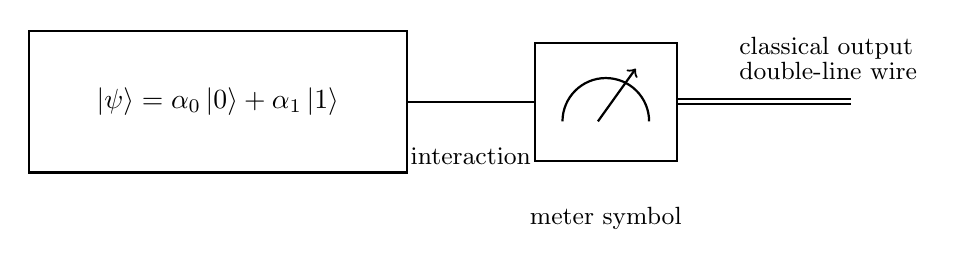
\begin{tikzpicture}[thick, baseline]

  % input state box
  \node[draw, minimum width=4.8cm, minimum height=1.8cm, align=center] (psi)
  {$\ket{\psi}=\alpha_0\ket{0}+\alpha_1\ket{1}$};

  % measurement box
  \node[draw, minimum width=1.8cm, minimum height=1.5cm, right=1.6cm of psi] (m) {};

  % quantum wire
  \draw (psi.east) -- (m.west);

  % classical output: double line
  \draw[double, double distance=1pt] (m.east) -- ++(2.2,0);

  % meter arc inside the box
  \draw ($(m.center)+(-0.55,-0.25)$)
        arc[start angle=180, end angle=0, radius=0.55];

  % meter needle
  \draw[->] ($(m.center)+(-0.10,-0.25)$)
        -- ($(m.center)+(0.38,0.42)$);

  % labels
  \node[below=0.45cm of m] {\small meter symbol};
  \node[below=0.45cm of psi.east, xshift=0.8cm] {\small interaction};
  \node[above right=0.15cm and 0.65cm of m.east, align=left]
  {\small classical output\\[-1mm]\small double-line wire};

\end{tikzpicture}
\end{center}

\end{tcolorbox}

We \uline{cannot} examine a qubit to determine its quantum state; instead, we can only acquire much more restricted information about the quantum state.

\subsection{Measurement (for a Single Qubit)}

\begin{tcolorbox}[propstyle, title={Postulate}]
When we measure a qubit in the state $\ket{\psi}=\alpha\ket{0}+\beta\ket{1}$, we get (on the classical display) either the result~0 with probability $|\alpha|^2$, or the result~1 with probability $|\beta|^2$. Measurement \emph{changes} the state, collapsing it from its superposition to the specific state consistent with the measurement result. Since the probabilities must sum to one, $|\alpha|^2+|\beta|^2=1$.
\end{tcolorbox}

If we rapidly and repeatedly keep measuring the same state, we can suppress its evolution and effectively freeze it (the quantum Zeno effect).

\begin{figure}[H]
    \centering
    \includegraphics[width=1\linewidth]{squbit.png}
    \caption{Geomtric Interpretation}
    \label{fig:placeholder}
\end{figure}

\paragraph{Example 1:} For $\ket{\psi}=\frac{1}{\sqrt{2}}(\ket{0}+e^{i\pi/6}\ket{1})$, the probability of getting 0 is $|1/\sqrt{2}|^2=1/2$, and the probability of getting 1 is $|e^{i\pi/6}/\sqrt{2}|^2=1/2$.

\paragraph{Example 2:} For $\ket{\psi}=\frac{2}{3}\ket{0}+\frac{1-2i}{3}\ket{1}$, probability of 0 is $|2/3|^2=4/9$, probability of 1 is $|1-2i|^2/9=5/9$.

\begin{tcolorbox}[propstyle, title={Postulate ,  General Two-State Measurement}]
Any measurement device for a two-state quantum system has two preferred orthonormal states $\{\ket{u},\ket{u^\perp}\}$ forming a basis. Measurement of state $\ket{v}=a\ket{u}+b\ket{u^\perp}$ yields $\ket{u}$ with probability $|a|^2$ and $\ket{u^\perp}$ with probability $|b|^2$, collapsing the state to the outcome.
\end{tcolorbox}

A second measurement with respect to the same basis returns the same result with probability~1. All measurement devices have associated bases: Z-basis $\{\ket{0},\ket{1}\}$ (z-axis), X-basis $\{\ket{+},\ket{-}\}$ (x-axis), Y-basis $\{\ket{i},\ket{-i}\}$ (y-axis). When we say ``measure a qubit'' without specification, we mean measurement in the computational basis.

\paragraph{Measurement in different bases.}
The state
\[
\ket{\psi}=\frac{\sqrt{3}}{2}\ket{0}+\frac{1}{2}\ket{1}
\]
measured in:

\begin{itemize}[nosep]
    \item \textbf{Z-basis:}
    Since the state is already written in the computational basis
    \[
    \{\ket{0},\ket{1}\},
    \]
    the probabilities are obtained by squaring the amplitudes:
    \[
    P(0)=\left|\frac{\sqrt{3}}{2}\right|^2=\frac{3}{4},
    \qquad
    P(1)=\left|\frac{1}{2}\right|^2=\frac{1}{4}.
    \]

    \item \textbf{X-basis:}
    The X-basis is
    \[
    \ket{+}=\frac{\ket{0}+\ket{1}}{\sqrt{2}},
    \qquad
    \ket{-}=\frac{\ket{0}-\ket{1}}{\sqrt{2}}.
    \]
    The amplitudes are
    \[
    \braket{+|\psi}
    =
    \frac{1}{\sqrt{2}}
    \left(
    \frac{\sqrt{3}}{2}+\frac{1}{2}
    \right)
    =
    \frac{\sqrt{3}+1}{2\sqrt{2}},
    \]
    \[
    \braket{-|\psi}
    =
    \frac{1}{\sqrt{2}}
    \left(
    \frac{\sqrt{3}}{2}-\frac{1}{2}
    \right)
    =
    \frac{\sqrt{3}-1}{2\sqrt{2}}.
    \]
    Therefore,
    \[
    P(+)
    =
    \left|\frac{\sqrt{3}+1}{2\sqrt{2}}\right|^2
    =
    \frac{(\sqrt{3}+1)^2}{8}
    =
    \frac{2+\sqrt{3}}{4},
    \]
    \[
    P(-)
    =
    \left|\frac{\sqrt{3}-1}{2\sqrt{2}}\right|^2
    =
    \frac{(\sqrt{3}-1)^2}{8}
    =
    \frac{2-\sqrt{3}}{4}.
    \]

    \item \textbf{Y-basis:}
    The Y-basis is
    \[
    \ket{i}=\frac{\ket{0}+i\ket{1}}{\sqrt{2}},
    \qquad
    \ket{-i}=\frac{\ket{0}-i\ket{1}}{\sqrt{2}}.
    \]
    The amplitudes are
    \[
    \braket{i|\psi}
    =
    \frac{1}{\sqrt{2}}
    \left(
    \frac{\sqrt{3}}{2}-i\frac{1}{2}
    \right)
    =
    \frac{\sqrt{3}-i}{2\sqrt{2}},
    \]
    \[
    \braket{-i|\psi}
    =
    \frac{1}{\sqrt{2}}
    \left(
    \frac{\sqrt{3}}{2}+i\frac{1}{2}
    \right)
    =
    \frac{\sqrt{3}+i}{2\sqrt{2}}.
    \]
    Therefore,
    \[
    P(i)
    =
    \left|\frac{\sqrt{3}-i}{2\sqrt{2}}\right|^2
    =
    \frac{3+1}{8}
    =
    \frac{1}{2},
    \]
    \[
    P(-i)
    =
    \left|\frac{\sqrt{3}+i}{2\sqrt{2}}\right|^2
    =
    \frac{3+1}{8}
    =
    \frac{1}{2}.
    \]
\end{itemize}

\paragraph{Implications:}
\begin{enumerate}[nosep]
\item \textbf{Quantum distinguishability:} It is not always possible to reliably distinguish arbitrary non-orthogonal states.
\item \textbf{Information content:} Even though a qubit can be in infinitely many superposition states, a single measurement yields at most one classical bit of information. An unknown quantum state cannot be fully determined from a single copy.
\end{enumerate}


\subsection{Non-Commutativity of Measurements}

Measuring observables in different orders generally yields different results. Consider a qubit in state $\ket{0}$ and two observables: $A$ (X-basis) and $B$ (Z-basis).

\paragraph{Sequence 1: Measure $A$ (X) first, then $B$ (Z).}
Measuring $\ket{0}$ in X-basis: $\Pr(\ket{+})=1/2$, $\Pr(\ket{-})=1/2$. If outcome is $\ket{+}$, measuring in Z-basis gives $\ket{0}$ or $\ket{1}$ each with probability $1/2$. Similarly for $\ket{-}$. All four outcomes $(+,0),(+,1),(-,0),(-,1)$ occur with probability $1/4$.

\paragraph{Sequence 2: Measure $B$ (Z) first, then $A$ (X).}
Measuring $\ket{0}$ in Z-basis: $\Pr(\ket{0})=1$, $\Pr(\ket{1})=0$. Outcome is $\ket{0}$ deterministically. Then measuring $\ket{0}$ in X-basis gives $\ket{+}$ or $\ket{-}$ each with probability $1/2$. Only two outcomes occur.

The measurement order matters because the first measurement collapses the state, affecting subsequent measurements.

\subsection{Heisenberg Uncertainty Principle}

\begin{tcolorbox}[propstyle, title={Theorem: Heisenberg Uncertainty Principle}]
For any two Hermitian operators $A$ and $B$ and any quantum state $\ket{\psi}$:
\[
\Delta(A)^2\,\Delta(B)^2 \ge \frac{1}{4}|\langle[A,B]\rangle|^2,
\]
where $\Delta(A)^2=\langle A^2\rangle - \langle A\rangle^2$ is the variance and $[A,B]=AB-BA$ is the commutator.
\end{tcolorbox}

\paragraph{Derivation.} Define $\tilde{A}=A-\langle A\rangle I$ and $\tilde{B}=B-\langle B\rangle I$ (deviations from means). Then $\Delta(A)^2=\langle\tilde{A}^2\rangle$ and $\Delta(B)^2=\langle\tilde{B}^2\rangle$.

Setting $\ket{u}=\tilde{A}\ket{\psi}$ and $\ket{v}=\tilde{B}\ket{\psi}$, the Cauchy--Schwarz inequality gives:
\[
\langle\tilde{A}^2\rangle\langle\tilde{B}^2\rangle = \braket{u|u}\braket{v|v} \ge |\braket{u|v}|^2 = |\langle\tilde{A}\tilde{B}\rangle|^2.
\]

Decomposing $\tilde{A}\tilde{B}=\frac{1}{2}[\tilde{A},\tilde{B}]+\frac{1}{2}\{\tilde{A},\tilde{B}\}$ into commutator and anti-commutator:
\begin{itemize}[nosep]
\item The commutator $[\tilde{A},\tilde{B}]=[A,B]$ is anti-Hermitian, so $\langle[A,B]\rangle$ is purely imaginary.
\item The anti-commutator $\{\tilde{A},\tilde{B}\}$ is Hermitian, so $\langle\{\tilde{A},\tilde{B}\}\rangle$ is real.
\end{itemize}

Therefore: $|\langle\tilde{A}\tilde{B}\rangle|^2 = \frac{1}{4}|\langle[A,B]\rangle|^2 + \frac{1}{4}|\langle\{\tilde{A},\tilde{B}\}\rangle|^2 \ge \frac{1}{4}|\langle[A,B]\rangle|^2$.

\paragraph{Application to position and momentum.} Since $[X,P]=i\hbar$: $\Delta(X)\Delta(P)\ge\hbar/2$.

\paragraph{Correct interpretation.} The uncertainty principle does \emph{not} mean that measuring $A$ ``disturbs'' $B$. Rather, if we prepare many identical copies and measure $A$ on some and $B$ on others, the product of standard deviations satisfies the inequality.

%% ============================================================
%% SECTION 4: Single-Qubit Quantum Gates
%% ============================================================
\newpage
\section{Single-Qubit Quantum Gates}
\textit{Gate} is the operator which flips the state of a qubit from state 0 to state 1 and vice versa.

This specification is not enough because specifying the action of the gate on the states \(|0\rangle\) and \(|1\rangle\) does not tell us what happens to superpositions of the states, i.e.:

\[
|\psi\rangle = \alpha |0\rangle + \beta |1\rangle
\]

A quantum gate \(U\) acts linearly on a qubit state. If
\[
|\psi\rangle = \alpha |0\rangle + \beta |1\rangle,
\]
then
\[
U|\psi\rangle
=
U(\alpha |0\rangle + \beta |1\rangle)
=
\alpha U|0\rangle + \beta U|1\rangle.
\]

Assume
\[
U|0\rangle =
\begin{pmatrix}
a \\ b
\end{pmatrix},
\qquad
U|1\rangle =
\begin{pmatrix}
c \\ d
\end{pmatrix}.
\]
Then
\[
U|\psi\rangle
=
\alpha
\begin{pmatrix}
a \\ b
\end{pmatrix}
+
\beta
\begin{pmatrix}
c \\ d
\end{pmatrix}
=
\begin{pmatrix}
a\alpha + c\beta \\
b\alpha + d\beta
\end{pmatrix}.
\]

Equivalently,
\[
U|\psi\rangle
=
(a\alpha + c\beta)|0\rangle
+
(b\alpha + d\beta)|1\rangle.
\]

Since the resulting state must remain normalized, the total probability must still be \(1\):
\[
|a\alpha + c\beta|^2 + |b\alpha + d\beta|^2 = 1.
\]
\subsection{Single-Qubit Gates}

Quantum gates are unitary matrices that transform qubit states. Since quantum gates are unitary, they are always reversible: $U^{-1}=U^\dagger$.

\begin{tcolorbox}[propstyle, title={Theorem: Quantum Gates Are Unitary}]
A matrix $U$ represents a valid quantum gate if and only if
$U^\dagger U=UU^\dagger=I$.
This ensures normalization is preserved: if
$\braket{\psi}{\psi}=1$, then for $\ket{\phi}=U\ket{\psi}$,
\[
\braket{\phi}{\phi}
=
\bra{\psi}U^\dagger U\ket{\psi}
=
\braket{\psi}{\psi}
=
1.
\]
\end{tcolorbox}

A quantum gate U is always reversible i.e. if we apply a quantum gate U, we can undo the operation by applying $U^\dagger$.

\subsection{Pauli and Phase Gates}

\subsubsection*{Identity Gate}
$I=\bigl(\begin{smallmatrix}1&0\\0&1\end{smallmatrix}\bigr)=\ket{0}\!\bra{0}+\ket{1}\!\bra{1}$. Does nothing: $I\ket{\psi}=\ket{\psi}$.

\subsubsection*{Pauli-$X$ Gate (NOT Gate, Bit Flip)}

\begin{tcolorbox}[defstyle, title={Definition: Pauli-$X$ Gate}]
\[
X = \begin{pmatrix}0&1\\1&0\end{pmatrix} = \ket{0}\!\bra{1}+\ket{1}\!\bra{0}.
\]
Action: $X\ket{0}=\ket{1}$, $X\ket{1}=\ket{0}$. On superposition: $X(\alpha\ket{0}+\beta\ket{1})=\beta\ket{0}+\alpha\ket{1}$. Called the \emph{bit flip} operator. $X^\dagger=X$, $X^2=I$.
\end{tcolorbox}

\subsubsection*{Pauli-$Z$ Gate (Phase Flip)}

\begin{tcolorbox}[defstyle, title={Definition: Pauli-$Z$ Gate}]
\[
Z = \begin{pmatrix}1&0\\0&-1\end{pmatrix} = \ket{0}\!\bra{0}-\ket{1}\!\bra{1}.
\]
Action: $Z\ket{0}=\ket{0}$, $Z\ket{1}=-\ket{1}$. On superposition: $Z(\alpha\ket{0}+\beta\ket{1})=\alpha\ket{0}-\beta\ket{1}$. Called the \emph{phase flip}. $Z^\dagger=Z$, $Z^2=I$.
\end{tcolorbox}

\subsubsection*{Pauli-$Y$ Gate}

\begin{tcolorbox}[defstyle, title={Definition: Pauli-$Y$ Gate}]
\[
Y = \begin{pmatrix}0&-i\\i&0\end{pmatrix} = -i\ket{0}\!\bra{1}+i\ket{1}\!\bra{0}.
\]
Action: $Y\ket{0}=i\ket{1}$, $Y\ket{1}=-i\ket{0}$. It is the ``bit-and-phase flip''. $Y^\dagger=Y$, $Y^2=I$.
\end{tcolorbox}

\subsubsection*{$S$ Gate and $T$ Gate}

\begin{tcolorbox}[defstyle, title={Definition: $S$ (Phase) Gate}]
\[
S = \begin{pmatrix}1&0\\0&i\end{pmatrix},\quad S\ket{\psi}=\alpha\ket{0}+i\beta\ket{1}=\alpha\ket{0}+e^{i\pi/2}\beta\ket{1}.
\]
$S^2=Z$, $S^4=I$.
\end{tcolorbox}

\begin{tcolorbox}[defstyle, title={Definition: $T$ ($\pi/8$) Gate}]
\[
T = \begin{pmatrix}1&0\\0&e^{i\pi/4}\end{pmatrix},\quad T\ket{\psi}=\alpha\ket{0}+e^{i\pi/4}\beta\ket{1}.
\]
$T^2=S$, $T^4=Z$, $T^8=I$. Called $\pi/8$ gate because $T=e^{i\pi/8}\bigl(\begin{smallmatrix}e^{-i\pi/8}&0\\0&e^{i\pi/8}\end{smallmatrix}\bigr)$.
\end{tcolorbox}

\subsection{Hadamard Gate}

\begin{tcolorbox}[defstyle, title={Definition: Hadamard Gate}]
\[
H = \frac{1}{\sqrt{2}}\begin{pmatrix}1&1\\1&-1\end{pmatrix},\quad H\ket{x}=\frac{\ket{0}+(-1)^x\ket{1}}{\sqrt{2}}.
\]
$H\ket{0}=\ket{+}$, $H\ket{1}=\ket{-}$. $H^\dagger=H$, $H^2=I$. Creates superpositions and implements quantum interference.
\end{tcolorbox}

\paragraph{Quantum interference:} $H(\alpha\ket{0}+\beta\ket{1})=\frac{\alpha+\beta}{\sqrt{2}}\ket{0}+\frac{\alpha-\beta}{\sqrt{2}}\ket{1}$. For $\ket{+}$: $H\ket{+}=\ket{0}$ (constructive on $\ket{0}$, destructive on $\ket{1}$). For $\ket{-}$: $H\ket{-}=\ket{1}$.

\paragraph{Combination example:} $ZSH\ket{0}=\frac{1}{\sqrt{2}}(\ket{0}-i\ket{1})$. Measuring in Z-basis gives $\ket{0}$ or $\ket{1}$ with equal probability $1/2$.

\subsection{Rotation Gates}

\begin{tcolorbox}[defstyle, title={Definition: Rotation Gates}]
\begin{align*}
R_x(\theta) &= e^{-i\theta X/2} = \begin{pmatrix}\cos\frac{\theta}{2}&-i\sin\frac{\theta}{2}\\-i\sin\frac{\theta}{2}&\cos\frac{\theta}{2}\end{pmatrix}, \\
R_y(\theta) &= e^{-i\theta Y/2} = \begin{pmatrix}\cos\frac{\theta}{2}&-\sin\frac{\theta}{2}\\\sin\frac{\theta}{2}&\cos\frac{\theta}{2}\end{pmatrix}, \\
R_z(\theta) &= e^{-i\theta Z/2} = \begin{pmatrix}e^{-i\theta/2}&0\\0&e^{i\theta/2}\end{pmatrix},\quad \mathrm{Ph}(\delta)=e^{i\delta}I.
\end{align*}
Key identity: For $A^2=I$: $e^{iAx}=\cos(x)I+i\sin(x)A$.
\end{tcolorbox}

$R_z(\alpha)$ advances the azimuthal angle $\phi$ by $\alpha$ on the Bloch sphere. A rotation by $2\pi$ gives a phase of $-1$ (not identity); $4\pi$ is needed to return to the original state (``Dirac's belt trick'').

\paragraph{Gates from rotations:}
\begin{itemize}[nosep]
\item $X = R_x(\pi)\cdot\mathrm{Ph}(\pi/2)$ (rotation of $180°$ about $x$-axis + global phase).
\item $Y = R_y(\pi)\cdot\mathrm{Ph}(\pi/2)$.
\item $Z = R_z(\pi)\cdot\mathrm{Ph}(\pi/2)$.
\item $S = R_z(\pi/2)\cdot\mathrm{Ph}(\pi/4)$; $S^2=Z$.
\item $T = R_z(\pi/4)\cdot\mathrm{Ph}(\pi/8)$; $T^2=S$.
\end{itemize}

\paragraph{Rotation about arbitrary axis:} For unit vector $\hat{n}=(n_x,n_y,n_z)$:
\[
R_{\hat{n}}(\theta)=\cos\frac{\theta}{2}\,I - i\sin\frac{\theta}{2}(n_x X+n_y Y+n_z Z).
\]
$H$ is a rotation of $180°$ about the $\hat{x}+\hat{z}$ axis.

\begin{tcolorbox}[propstyle, title={Theorem: $Z$--$Y$ Decomposition}]
Any single-qubit unitary $U$ can be written as $U=e^{i\alpha}R_z(\beta)\,R_y(\gamma)\,R_z(\delta)$ for real $\alpha,\beta,\gamma,\delta$.
\end{tcolorbox}

\begin{tcolorbox}[propstyle, title={Theorem: Arbitrary Unitary Operator}]
An arbitrary single-qubit unitary $U$ can be written as $U=e^{i\alpha}R_{\hat{n}}(\theta)$ for some real $\alpha,\theta$ and unit vector $\hat{n}$.
\end{tcolorbox}





\paragraph{Simplifying consecutive applications:} $X^{1001}=X^{1000}\cdot X=(X^2)^{500}\cdot X=I^{500}\cdot X=X$.

\subsubsection*{Pauli $Y$ Gate Action}

$Y(\alpha\ket{0}+\beta\ket{1})=\bigl(\begin{smallmatrix}0&-i\\i&0\end{smallmatrix}\bigr)\bigl(\begin{smallmatrix}\alpha\\\beta\end{smallmatrix}\bigr)=\bigl(\begin{smallmatrix}-i\beta\\i\alpha\end{smallmatrix}\bigr)=-i\beta\ket{0}+i\alpha\ket{1}$.

This is equivalent to $-i(\alpha\ket{0}-\beta\ket{1})$ with different phase structure. $Y$ flips both the bit and the relative phase simultaneously.

\subsubsection*{$S$ Gate: Detailed Verification}

$S^\dagger=\bigl(\begin{smallmatrix}1&0\\0&-i\end{smallmatrix}\bigr)$. Verify: $SS^\dagger=\bigl(\begin{smallmatrix}1&0\\0&i\end{smallmatrix}\bigr)\bigl(\begin{smallmatrix}1&0\\0&-i\end{smallmatrix}\bigr)=\bigl(\begin{smallmatrix}1&0\\0&1\end{smallmatrix}\bigr)=I$. Also $S^\dagger S=I$.

Action: $S(\alpha\ket{0}+\beta\ket{1})=\alpha\ket{0}+i\beta\ket{1}=\alpha\ket{0}+e^{i\pi/2}\beta\ket{1}$.

On Bloch sphere: rotation of $90°$ about $z$-axis. $S^2=\bigl(\begin{smallmatrix}1&0\\0&-1\end{smallmatrix}\bigr)=Z$. Need to apply $S$ four times to return: $S^4=Z^2=I$.

\subsubsection*{Hadamard: Interference Examples}

The Hadamard gate creates interference:
\[
H(\alpha\ket{0}+\beta\ket{1})=\frac{\alpha+\beta}{\sqrt{2}}\ket{0}+\frac{\alpha-\beta}{\sqrt{2}}\ket{1}.
\]

\textbf{Positive interference:} $H\ket{+}=H\bigl(\frac{1}{\sqrt{2}}(\ket{0}+\ket{1})\bigr)=\frac{1/\sqrt{2}+1/\sqrt{2}}{\sqrt{2}}\ket{0}+\frac{1/\sqrt{2}-1/\sqrt{2}}{\sqrt{2}}\ket{1}=\ket{0}$.

The two amplitudes add constructively for $\ket{0}$ (probability goes from 50\% to 100\%) and destructively for $\ket{1}$ (50\% to 0\%).

\textbf{Negative interference:} $H\ket{-}=\ket{1}$. Constructive on $\ket{1}$, destructive on $\ket{0}$.

\textbf{Key insight:} $\ket{+}$ and $\ket{-}$ have identical measurement probabilities in the Z-basis ($1/2$ each), but $H$ distinguishes them, demonstrating that the relative phase is physically observable.

\subsubsection*{Gate Combination: Probability Computation}

For the circuit $H$--$T$--$H$ applied to $\ket{0}$:
\[
HTH\ket{0}=HT\ket{+}=H\frac{1}{\sqrt{2}}(\ket{0}+e^{i\pi/4}\ket{1})=\frac{1}{2}\bigl[(1+e^{i\pi/4})\ket{0}+(1-e^{i\pi/4})\ket{1}\bigr].
\]
Using $e^{i\pi/4}=\frac{1+i}{\sqrt{2}}$ and Euler's formula:
\[
\Pr(0)=\frac{|1+e^{i\pi/4}|^2}{4}=\frac{2+2\cos(\pi/4)}{4}=\frac{2+\sqrt{2}}{4}=\cos^2(\pi/8).
\]

\subsubsection*{$R_z$ Gate Derivation on Bloch Sphere}

For $\ket{\psi}=\cos\frac{\theta}{2}\ket{0}+e^{i\phi}\sin\frac{\theta}{2}\ket{1}$:
\begin{align*}
R_z(\alpha)\ket{\psi}&=\begin{pmatrix}e^{-i\alpha/2}&0\\0&e^{i\alpha/2}\end{pmatrix}\begin{pmatrix}\cos\frac{\theta}{2}\\e^{i\phi}\sin\frac{\theta}{2}\end{pmatrix}=\begin{pmatrix}e^{-i\alpha/2}\cos\frac{\theta}{2}\\e^{i(\phi+\alpha/2)}\sin\frac{\theta}{2}\end{pmatrix}\\
&=e^{-i\alpha/2}\bigl(\cos\frac{\theta}{2}\ket{0}+e^{i(\phi+\alpha)}\sin\frac{\theta}{2}\ket{1}\bigr)\equiv\cos\frac{\theta}{2}\ket{0}+e^{i(\phi+\alpha)}\sin\frac{\theta}{2}\ket{1}.
\end{align*}
The angle $\phi$ advances by $\alpha$: a rotation about the $z$-axis.

\paragraph{$2\pi$ rotation anomaly:} $R_z(2\pi)\ket{\psi}=e^{-i\pi}\ket{\psi}=-\ket{\psi}\neq\ket{\psi}$. A $4\pi$ rotation is needed: $R_z(4\pi)=e^{-2\pi i}I=I$. This has no classical analogue (``Dirac belt trick'').

\subsection{Evolution}

\begin{tcolorbox}[propstyle, title={Postulate}]
The evolution of a closed quantum system is described by a unitary transformation: $\ket{\psi(t_2)}=U(t_1,t_2)\ket{\psi(t_1)}$.
\end{tcolorbox}

\begin{tcolorbox}[propstyle, title={Schr\"odinger Equation}]
$i\hbar\frac{d\ket{\psi}}{dt}=H\ket{\psi}$, where $H$ is the Hamiltonian ($H=H^\dagger$). Setting $\hbar=1$: $U(t_1,t_2)=\exp[-iH(t_2-t_1)]$.
\end{tcolorbox}
%% ============================================================
%% SECTION 5: Composite Systems and Multi-Qubit Measurement
%% ============================================================
\section{Composite Systems and Multi-Qubit Measurement}

\subsection{Composite Systems}

\begin{tcolorbox}[propstyle, title={Postulate}]
The state space of a composite physical system is the \emph{tensor product} of the component state spaces. If system $i$ is in state $\ket{\psi_i}$, the joint state is $\ket{\psi_1}\otimes\ket{\psi_2}\otimes\cdots\otimes\ket{\psi_n}$.
\end{tcolorbox}

For two qubits, $\dim(\mathcal{H}_A\otimes\mathcal{H}_B)=2\times 2=4$. Standard basis: $\{\ket{00},\ket{01},\ket{10},\ket{11}\}$. For $n$ qubits: $\dim=2^n$. A general state: $\ket{\psi}=\sum_{j=0}^{2^n-1}c_j\ket{j}$ with $\sum|c_j|^2=1$.

\paragraph{Notation:} Binary basis $\ket{x_{n-1}\cdots x_0}$ or decimal $\ket{x}$ where $x=\sum x_k 2^k$. Little endian (Qiskit): rightmost qubit is zeroth. Big endian (Nielsen\&Chuang): leftmost qubit is zeroth.

There is \textbf{no Bloch sphere} for multi-qubit states.

\subsection{Multi-Qubit Measurement}

Two qubits can exist in a superposition of the four states of the standard basis:
\[
|00\rangle,\ |01\rangle,\ |10\rangle,\ |11\rangle.
\]

A general two-qubit state can be written as
\[
|\psi\rangle
=
c_{00}|00\rangle
+
c_{01}|01\rangle
+
c_{10}|10\rangle
+
c_{11}|11\rangle.
\]

Equivalently,
\[
|\psi\rangle
=
\sum_{i,j \in \{0,1\}} c_{ij}|ij\rangle.
\]

When both qubits are measured, the outcome \(|ij\rangle\) is obtained with probability
\[
P(ij) = |c_{ij}|^2.
\]

Since the total probability must be equal to \(1\), the coefficients satisfy
\[
\sum_{i,j \in \{0,1\}} |c_{ij}|^2 = 1.
\]

\paragraph{Measuring individual qubits:} Measuring only the first qubit of $\ket{\psi}$: get $\ket{0}$ with probability $|c_0|^2+|c_1|^2$, leaving post-measurement state $\frac{c_0\ket{00}+c_1\ket{01}}{\sqrt{|c_0|^2+|c_1|^2}}$; get $\ket{1}$ with probability $|c_2|^2+|c_3|^2$, leaving $\frac{c_2\ket{10}+c_3\ket{11}}{\sqrt{|c_2|^2+|c_3|^2}}$.

\paragraph{Worked example:} For $\ket{\psi}=\frac{1}{\sqrt{2}}\ket{00}+\frac{1}{2}\ket{01}+\frac{\sqrt{3}}{4}\ket{10}+\frac{1}{4}\ket{11}$, measuring the left qubit:
\begin{itemize}[nosep]
\item $\Pr(0)=\frac{1}{2}+\frac{1}{4}=\frac{3}{4}$, post-state: $\sqrt{\frac{2}{3}}\ket{00}+\frac{1}{\sqrt{3}}\ket{01}$.
\item $\Pr(1)=\frac{3}{16}+\frac{1}{16}=\frac{1}{4}$, post-state: $\frac{\sqrt{3}}{2}\ket{10}+\frac{1}{2}\ket{11}$.
\end{itemize}

\subsubsection*{Projection Operators for Measurement}

\begin{figure}[H]
    \centering
    \includegraphics[width=0.8\linewidth]{projop.png}
    \caption{Geometric interpretation}
    \label{fig:placeholder}
\end{figure}

If \(|\psi\rangle\) is a unit vector in the plane, i.e. \(V=\mathbb{R}^2\), then \(S\) can be the subspace spanned by \(|0\rangle\) and \(S^\perp\) the subspace generated by \(|1\rangle\). Obviously,
\[
V = S \oplus S^\perp .
\]

From now on, we slightly change the notation: we use \(S_0\) and \(S_1\) instead of \(S\) and \(S^\perp\), respectively. Therefore,
\[
V = S_0 \oplus S_1 .
\]

\begin{tcolorbox}[propstyle, title={Postulate}]
A measuring device with decomposition $V=S_1\oplus S_2\oplus\cdots\oplus S_k$ acting on $\ket{\psi}$ outputs label $i$ with probability $p(i)=\|P_i\ket{\psi}\|^2=\bra{\psi}P_i\ket{\psi}$ and leaves the state as $\frac{P_i\ket{\psi}}{\|P_i\ket{\psi}\|}$, where $P_i$ is the projector onto $S_i$.
\end{tcolorbox}

\paragraph{Example 2 (standard basis):} $P_0=\ket{0}\!\bra{0}$, $P_1=\ket{1}\!\bra{1}$. $P_0(\alpha\ket{0}+\beta\ket{1})=\alpha\ket{0}$. Probability: $|\alpha|^2$.

\paragraph{Example 4 (bit equality):} $V=S_1\oplus S_2$ where $S_1=\mathrm{span}\{\ket{00},\ket{11}\}$, $S_2=\mathrm{span}\{\ket{01},\ket{10}\}$. $P_1=\ket{00}\!\bra{00}+\ket{11}\!\bra{11}$. Measures whether two bits are equal without determining their values.

\paragraph{Example 5 (Bell basis):} $V=S_{\Phi^+}\oplus S_{\Phi^-}\oplus S_{\Psi^+}\oplus S_{\Psi^-}$. Measuring $\ket{00}$: $\ket{00}=\frac{1}{\sqrt{2}}(\ket{\Phi^+}+\ket{\Phi^-})$, so get $\ket{\Phi^+}$ or $\ket{\Phi^-}$ each with probability $1/2$.



\subsubsection*{Hermitian Operator Formalism for Measurement}
An \textit{observable} in Quantum Mechanics is a physical property of a system that can be measured, such as position, momentum, energy or angular momentum.
Observables are represented by Hermitian operators.

In Quantum Computing, an \textit{observable} is associated with a Hermitian operator, and we interpret the eigenvalues of that operator as the possible results of a measurement.\\
 \hspace*{15pt}Therefore, the act of reading a quantum state is thought of as an experimental determination of the value of some observable of the system.

\begin{tcolorbox}
    [propstyle, title={Postulate}]
 A quantum measurement is specified by a Hermitian operator \(O\), called an observable.

The possible outcomes of measuring a state \(|\psi\rangle\) are labeled by the eigenvalues \(\lambda_i\) of \(O\).

The probability of obtaining the outcome labeled by \(\lambda_i\) is
\[
p_i = \|P_i|\psi\rangle\|^2,
\]
where \(P_i\) is the projector onto the eigenspace associated with \(\lambda_i\).

After the measurement, the state collapses to the normalized projection
\[
|\psi_i\rangle
=
\frac{P_i|\psi\rangle}{\|P_i|\psi\rangle\|}
=
\frac{P_i|\psi\rangle}
{\sqrt{\langle \psi | P_i | \psi \rangle}}.
\]

Thus, the post-measurement state lies in the \(\lambda_i\)-eigenspace of \(O\).
\end{tcolorbox}

Any Hermitian operator $O:V\to V$ with distinct eigenvalues $\lambda_1,\dots,\lambda_k$ determines a unique eigenspace decomposition $V=S_1\oplus\cdots\oplus S_k$. Conversely, given any decomposition and distinct reals $\lambda_i$, the operator $O=\sum_i\lambda_i P_i$ is Hermitian with this decomposition.

The eigenvalues are merely \emph{labels} for outcomes. The Hermitian operator is a ``bookkeeping trick'' for specifying the measurement; the projectors $P_j$, not $O$ itself, act on states.



\subsection{Pauli Matrices and Projectors}

Each Pauli matrix $\sigma_i$ (with $i = x, y, z$) is Hermitian with eigenvalues $\pm 1$.
When measuring an observable represented by a Hermitian operator, the possible outcomes
correspond to its eigenvalues, and the measurement is described by the projectors onto
the corresponding eigenspaces. For any Pauli matrix $\sigma$, these projectors are
compactly written as:
\begin{equation}
    P_{\pm} = \frac{1}{2}(I \pm \sigma)
\end{equation}

\subsubsection*{Projectors for each Pauli matrix}

\textbf{For $\sigma_z = Z = \begin{pmatrix} 1 & 0 \\ 0 & -1 \end{pmatrix}$},
with eigenvectors $|0\rangle$ (eigenvalue $+1$) and $|1\rangle$ (eigenvalue $-1$):
\begin{equation}
    P_{+1}^{(z)} = |0\rangle\langle 0| = \begin{pmatrix} 1 & 0 \\ 0 & 0 \end{pmatrix}, \qquad
    P_{-1}^{(z)} = |1\rangle\langle 1| = \begin{pmatrix} 0 & 0 \\ 0 & 1 \end{pmatrix}
\end{equation}

\textbf{For $\sigma_x = X = \begin{pmatrix} 0 & 1 \\ 1 & 0 \end{pmatrix}$},
with eigenvectors $|{+}\rangle = \frac{1}{\sqrt{2}}\begin{pmatrix}1\\1\end{pmatrix}$ (eigenvalue $+1$)
and $|{-}\rangle = \frac{1}{\sqrt{2}}\begin{pmatrix}1\\-1\end{pmatrix}$ (eigenvalue $-1$):
\begin{equation}
    P_{+}^{(x)} = \frac{1}{2}\begin{pmatrix} 1 & 1 \\ 1 & 1 \end{pmatrix}, \qquad
    P_{-}^{(x)} = \frac{1}{2}\begin{pmatrix} 1 & -1 \\ -1 & 1 \end{pmatrix}
\end{equation}

\textbf{For $\sigma_y$}, the projectors are:
\begin{equation}
    P_{+i}^{(y)} = \frac{1}{2}\begin{pmatrix} 1 & -i \\ i & 1 \end{pmatrix}, \qquad
    P_{-i}^{(y)} = \frac{1}{2}\begin{pmatrix} 1 & +i \\ -i & 1 \end{pmatrix}
\end{equation}

In general, for any Pauli matrix $\sigma_i$, the projectors corresponding to outcomes $\pm 1$ are:
\begin{equation}
    P_{\pm}^{(i)} = \frac{1}{2}(I \pm \sigma_i)
\end{equation}
These projectors completely specify the measurement operations associated with the Pauli observables.

For any direct sum decomposition $V=S_1\oplus S_2\oplus\cdots\oplus S_k$ into orthogonal subspaces, there are $k$ projection operators $P_i:V\to S_i$ satisfying $P_i\ket{v}=\ket{s_i}$ where $\ket{\psi}=\ket{s_1}+\ket{s_2}+\cdots+\ket{s_k}$.

\begin{tcolorbox}[propstyle, title={Measurement Postulate (Complete Projective Form)}]
A measuring device with associated decomposition $V=S_1\oplus\cdots\oplus S_k$ acting on state $\ket{\psi}$ outputs label $i\in\{1,\dots,k\}$ with probability:
\[
p(i) = \|P_i\ket{\psi}\|^2 = \bra{\psi}P_i^\dagger P_i\ket{\psi} = \bra{\psi}P_i\ket{\psi}
\]
and leaves the system in the normalized state:
\[
\ket{\psi_i} = \frac{P_i\ket{\psi}}{\|P_i\ket{\psi}\|} = \frac{P_i\ket{\psi}}{\sqrt{\bra{\psi}P_i\ket{\psi}}}.
\]
\end{tcolorbox}

\paragraph{Example 2: Single qubit in standard basis.}
$V=S_0\oplus S_1$ with $S_0=\mathrm{span}\{\ket{0}\}$, $S_1=\mathrm{span}\{\ket{1}\}$. Projectors: $P_0=\ket{0}\!\bra{0}$, $P_1=\ket{1}\!\bra{1}$. For $\ket{\psi}=a\ket{0}+b\ket{1}$:
\begin{align*}
P_0\ket{\psi} &= \ket{0}\!\bra{0}(a\ket{0}+b\ket{1}) = a\ket{0}, & \|P_0\ket{\psi}\|^2 &= |a|^2,\\
P_1\ket{\psi} &= \ket{1}\!\bra{1}(a\ket{0}+b\ket{1}) = b\ket{1}, & \|P_1\ket{\psi}\|^2 &= |b|^2.
\end{align*}
The result $\ket{0}$ occurs with probability $|a|^2$ and $\ket{1}$ with probability $|b|^2$. Since $e^{i\theta}\ket{0}\equiv\ket{0}$, the post-measurement state is simply $\ket{0}$ or $\ket{1}$.

\paragraph{Example 3: Two-qubit full standard basis measurement.}
$V=S_{00}\oplus S_{01}\oplus S_{10}\oplus S_{11}$. Projectors $P_{ij}=\ket{ij}\!\bra{ij}$. For $\ket{\psi}=a_{00}\ket{00}+a_{01}\ket{01}+a_{10}\ket{10}+a_{11}\ket{11}$:
\[
P_{ij}\ket{\psi}=a_{ij}\ket{ij},\quad \|P_{ij}\ket{\psi}\|^2=|a_{ij}|^2.
\]

\paragraph{Example 4: Bit equality measurement.}
$V=S_1\oplus S_2$ where $S_1=\mathrm{span}\{\ket{00},\ket{11}\}$ (equal bits) and $S_2=\mathrm{span}\{\ket{01},\ket{10}\}$ (unequal bits).
\begin{align*}
P_1 &= \ket{00}\!\bra{00}+\ket{11}\!\bra{11}, & P_2 &= \ket{01}\!\bra{01}+\ket{10}\!\bra{10}.
\end{align*}
For general state:
\begin{align*}
P_1\ket{\psi} &= a_{00}\ket{00}+a_{11}\ket{11}, & \|P_1\ket{\psi}\|^2 &= |a_{00}|^2+|a_{11}|^2,\\
P_2\ket{\psi} &= a_{01}\ket{01}+a_{10}\ket{10}, & \|P_2\ket{\psi}\|^2 &= |a_{01}|^2+|a_{10}|^2.
\end{align*}
Outcome~1 tells us bits are equal (but not which value); outcome~2 tells us they differ.

\paragraph{Example 5: Bell basis measurement.}
Projectors: $P_{\Phi^+}=\ket{\Phi^+}\!\bra{\Phi^+}$, etc. Measuring $\ket{00}$: since $\ket{00}=\frac{1}{\sqrt{2}}(\ket{\Phi^+}+\ket{\Phi^-})$, we get $\ket{\Phi^+}$ with prob $1/2$ and $\ket{\Phi^-}$ with prob $1/2$.

\paragraph{Example 6:} $Z=\ket{0}\!\bra{0}-\ket{1}\!\bra{1}$ specifies Z-basis measurement. Eigenvalues: $+1$ (for $\ket{0}$), $-1$ (for $\ket{1}$).

\paragraph{Example 7:} $X=\ket{+}\!\bra{+}-\ket{-}\!\bra{-}$ specifies X-basis measurement. Eigenvalues: $+1$ (for $\ket{+}$), $-1$ (for $\ket{-}$).

\paragraph{Example 8:} $A=1\ket{00}\!\bra{00}+2\ket{01}\!\bra{01}+3\ket{10}\!\bra{10}+5\ket{11}\!\bra{11}$ specifies full standard-basis measurement with arbitrary distinct labels. Matrix: $\mathrm{diag}(1,2,3,5)$. Any other choice of distinct eigenvalues (e.g., 73, 50, $-3$, 23) also works.

\paragraph{Example 9:} $B=\alpha(\ket{00}\!\bra{00}+\ket{01}\!\bra{01})+\beta(\ket{10}\!\bra{10}+\ket{11}\!\bra{11})$ with $\alpha\neq\beta$ specifies measurement of the first qubit.

\paragraph{Example 10:} $C=2(\ket{00}\!\bra{00}+\ket{11}\!\bra{11})+3(\ket{01}\!\bra{01}+\ket{10}\!\bra{10})$ specifies bit-equality measurement.

Important: quantum measurement is NOT modeled by the action of $O$ on a state. Direct multiplication $Z\ket{\psi}$ does not give a valid post-measurement state. For example, $Z\bigl(\begin{smallmatrix}0\\0\end{smallmatrix}\bigr)=\bigl(\begin{smallmatrix}0\\0\end{smallmatrix}\bigr)$ is the zero vector, not a valid state.

%% ============================================================
%% SECTION 6: Product States and Entangled States
%% ============================================================
\section{Product States and Entangled States}

\subsection{Separable vs Entangled States}

\begin{tcolorbox}[defstyle, title={Definition: Bipartite State}]
A \textbf{bipartite state} is a quantum state of a composite system consisting of two subsystems $A$ and $B$, whose joint Hilbert space is the tensor product $\mathcal{H}_{AB}=\mathcal{H}_A\otimes\mathcal{H}_B$. A pure bipartite state is a vector $\ket{\psi}_{AB}\in\mathcal{H}_A\otimes\mathcal{H}_B$; a mixed bipartite state is a density operator $\rho_{AB}$ on $\mathcal{H}_A\otimes\mathcal{H}_B$.
\end{tcolorbox}

\begin{tcolorbox}[defstyle, title={Definition: Separable and Entangled States}]
A bipartite state is \textbf{separable} (product state) if $\ket{\psi}=\ket{\psi_A}\otimes\ket{\psi_B}$; otherwise it is \textbf{entangled}.
\end{tcolorbox}

\begin{tcolorbox}[defstyle, title={Definition: Maximally Entangled State}]
A pure bipartite state $\ket{\psi}_{AB}\in\mathcal{H}_A\otimes\mathcal{H}_B$ with $\dim\mathcal{H}_A=\dim\mathcal{H}_B=d$ is \textbf{maximally entangled} if its reduced density operator is maximally mixed:
\[
\rho_A = \mathrm{Tr}_B\!\left(\ket{\psi}\!\bra{\psi}\right) = \frac{I}{d}.
\]
Equivalently, all Schmidt coefficients are equal: $\lambda_i=1/\sqrt{d}$ for all $i=1,\dots,d$.
\end{tcolorbox}

\begin{tcolorbox}[defstyle, title={Definition: Bell States (EPR Pairs)}]
The four maximally entangled two-qubit states:
\begin{align*}
\ket{\Phi^+}&=\tfrac{1}{\sqrt{2}}(\ket{00}+\ket{11}), & \ket{\Phi^-}&=\tfrac{1}{\sqrt{2}}(\ket{00}-\ket{11}),\\
\ket{\Psi^+}&=\tfrac{1}{\sqrt{2}}(\ket{01}+\ket{10}), & \ket{\Psi^-}&=\tfrac{1}{\sqrt{2}}(\ket{01}-\ket{10}).
\end{align*}
\end{tcolorbox}
$\ket{\Phi^+}$ cannot be factored: if $\ket{\Phi^+}=(\alpha_1\ket{0}+\beta_1\ket{1})\otimes(\alpha_0\ket{0}+\beta_0\ket{1})$, matching coefficients gives $\alpha_1\alpha_0=1/\sqrt{2}$, $\alpha_1\beta_0=0$, $\beta_1\alpha_0=0$, $\beta_1\beta_0=1/\sqrt{2}$, which is contradictory.

Local operations on one qubit transform Bell states: $(I\otimes I)\ket{\Phi^+}=\ket{\Phi^+}$, $(X\otimes I)\ket{\Phi^+}=\ket{\Psi^+}$, $(Z\otimes I)\ket{\Phi^+}=\ket{\Phi^-}$, $(iY\otimes I)\ket{\Phi^+}=\ket{\Psi^-}$.

\subsubsection*{Product States vs.\ Entangled States}

\begin{tcolorbox}[defstyle, title={Definition: Product (Separable) States}]
A state $\ket{\psi}_{AB}$ is a \textbf{product state} if it can be factored: $\ket{\psi}_{AB}=\ket{\phi}_A\otimes\ket{\chi}_B$. Otherwise it is \textbf{entangled}.
\end{tcolorbox}

\paragraph{Separability test (2 qubits):} Write $\ket{\psi}=c_{00}\ket{00}+c_{01}\ket{01}+c_{10}\ket{10}+c_{11}\ket{11}$. It is separable iff $c_{00}c_{11}=c_{01}c_{10}$ (the ``determinant test'' on the $2\times 2$ coefficient matrix).

\paragraph{Example:} $\frac{1}{\sqrt{2}}(\ket{01}+\ket{10})$: coefficient matrix $\bigl(\begin{smallmatrix}0&1/\sqrt{2}\\1/\sqrt{2}&0\end{smallmatrix}\bigr)$, determinant $=-1/2\neq 0$. Entangled.

\subsection{Entangled States}

\paragraph{Monogamy of entanglement.} If qubits $A$ and $B$ are maximally entangled, they cannot be entangled with a third qubit $C$. The full three-qubit state must factor as $\ket{\text{EPR}}_{AB}\otimes\ket{\chi}_C$. This is proven by expanding in the diagonal basis and showing that correlations with $C$ vanish.

\[
\{\text{Bell states}\} \subset \{\text{maximally entangled two-qubit states}\}
\]
For pure states:
\[
\text{product state} \iff \text{separable state} \iff \text{not entangled}.
\]

For mixed states:
\[
\text{product states} \subset \text{separable states} \subset \text{not entangled states}.
\]

Equivalently:
\[
\text{product state} \Rightarrow \text{separable state} \Rightarrow \text{not entangled}.
\]
%%

\subsubsection{Non-Locality}
Entangled states are non-local: measuring one subsystem affects the joint state, and its outcomes are correlated with those of the distant subsystem.

Likewise, separable states are considered local, since they allow full segregation of the actions on separate qubit states.

%% SECTION 7: Quantum Circuit Model
%% ============================================================
\newpage
\section{Quantum Circuit Model}

\begin{tcolorbox}
    [defstyle, title={Definition}]
    The \textbf{depth} of a circuit is the longest path in the circuit
\end{tcolorbox}

Sometimes circuits need to be \textit{transpiled}, translated in a circuit executable on a physical hardware using native gates. The transpilation process is automatically handled by \textbf{Qiskit}.

The transpilation process can significantly increase the depth of the original circuit.

\subsection{Controlled Gates}

\begin{tcolorbox}[defstyle, title={Definition: CNOT (Controlled-NOT) Gate}]
Two-qubit gate with control ($c$) and target ($t$):
\[
\mathrm{CNOT}\ket{c,t}=\ket{c,t\oplus c},\quad \mathrm{CNOT}=\ket{0}\!\bra{0}\otimes I+\ket{1}\!\bra{1}\otimes X=\begin{pmatrix}1&0&0&0\\0&1&0&0\\0&0&0&1\\0&0&1&0\end{pmatrix}.
\]
$\mathrm{CNOT}^\dagger=\mathrm{CNOT}$, $\mathrm{CNOT}^2=I$.
\end{tcolorbox}

\begin{figure}[H]
    \centering
    \includegraphics[width=0.75\linewidth]{cnot.png}
    \caption{CNOT gate}
    \label{fig:placeholder}
\end{figure}

\begin{figure}[H]
    \centering
    \includegraphics[width=1\linewidth]{solid.png}
    \caption{Action of the gate}
    \label{fig:placeholder}
\end{figure}
\begin{tcolorbox}[defstyle, title={Definition: Controlled-$U$ Gate}]
$CU=\ket{0}\!\bra{0}\otimes I+\ket{1}\!\bra{1}\otimes U=\begin{pmatrix}I&0\\0&U\end{pmatrix}$. If control is $\ket{1}$, apply $U$ to target; otherwise leave target alone.
\end{tcolorbox}

Important controlled gates: $CZ$ (controlled-$Z$), $CS$ (controlled-$S$), $CT$ (controlled-$T$).

\paragraph{Swapping roles:} $(C^\downarrow)U$ means target on top, control on bottom. $(C^\downarrow)\mathrm{CNOT}$ has matrix with different structure. $\mathrm{CNOT}\cdot(C^\downarrow)\mathrm{CNOT}\cdot\mathrm{CNOT}=\mathrm{SWAP}$.

\paragraph{SWAP Gate:} $\mathrm{SWAP}\ket{x,y}=\ket{y,x}$, $\mathrm{SWAP}=\ket{00}\!\bra{00}+\ket{01}\!\bra{10}+\ket{10}\!\bra{01}+\ket{11}\!\bra{11}$.

\paragraph{Quantum entanglement from CNOT:} $\mathrm{CNOT}(\ket{+}\otimes\ket{0})=\frac{1}{\sqrt{2}}(\ket{00}+\ket{11})=\ket{\Phi^+}$. A separable input does not always produce a separable output.

\subsubsection*{CNOT Analysis}

The CNOT gate acts on the general two-qubit state $\ket{\psi}=c_0\ket{00}+c_1\ket{01}+c_2\ket{10}+c_3\ket{11}$:
\[
\mathrm{CNOT}\ket{\psi} = c_0\ket{00}+c_1\ket{01}+c_3\ket{10}+c_2\ket{11}.
\]
The amplitudes of $\ket{10}$ and $\ket{11}$ are swapped. In outer product form:
\[
\mathrm{CNOT} = \ket{00}\!\bra{00}+\ket{01}\!\bra{01}+\ket{10}\!\bra{11}+\ket{11}\!\bra{10} = \ket{0}\!\bra{0}\otimes I + \ket{1}\!\bra{1}\otimes X.
\]

\paragraph{Entanglement generation:} Starting with $\ket{+}\otimes\ket{0}=\frac{1}{\sqrt{2}}(\ket{00}+\ket{10})$:
\[
\mathrm{CNOT}\frac{1}{\sqrt{2}}(\ket{00}+\ket{10}) = \frac{1}{\sqrt{2}}(\ket{00}+\ket{11}) = \ket{\Phi^+}.
\]
A separable input becomes entangled. However, $\mathrm{CNOT}(\ket{1}\otimes\frac{1}{\sqrt{2}}(\ket{0}+\ket{1}))=\ket{1}\otimes\frac{1}{\sqrt{2}}(\ket{1}+\ket{0})$, still separable, because the control is a basis state.

\subsubsection*{Controlled-$U$ Gate}

For arbitrary single-qubit unitary $U$ with $U\ket{0}=U_{00}\ket{0}+U_{10}\ket{1}$ and $U\ket{1}=U_{01}\ket{0}+U_{11}\ket{1}$:
\begin{align*}
CU\ket{00}&=\ket{00}, & CU\ket{01}&=\ket{01}, \\
CU\ket{10}&=\ket{1}\otimes U\ket{0}=U_{00}\ket{10}+U_{10}\ket{11}, & CU\ket{11}&=\ket{1}\otimes U\ket{1}=U_{01}\ket{10}+U_{11}\ket{11}.
\end{align*}
Matrix: $CU=\begin{pmatrix}1&0&0&0\\0&1&0&0\\0&0&U_{00}&U_{01}\\0&0&U_{10}&U_{11}\end{pmatrix}$.

\subsubsection*{Controlled-$X$ Gate}
For $U=X$: $U_{00}=U_{11}=0$, $U_{01}=U_{10}=1$.
\begin{align*}
CX\ket{00}&=\ket{00}, & CX\ket{01}&=\ket{01}, \\
CX\ket{10}&=\ket{11}, & CX\ket{11}&=\ket{10}.
\end{align*}
Matrix: $CX = CNOT =\begin{pmatrix}1&0&0&0\\0&1&0&0\\0&0&0&1\\0&0&1&0\end{pmatrix}$.

In Dirac notation: $CX = \ket{00}\bra{00}+\ket{01}\bra{01}+\ket{10}\bra{11}+\ket{11}\bra{10}$.

Action on a general state $\ket{\psi}=\alpha\ket{00}+\beta\ket{01}+\gamma\ket{10}+\delta\ket{11}$:
\[
CX\ket{\psi} = \alpha\ket{0}\ket{0}+\beta\ket{0}\ket{1}+\delta\ket{1}\ket{0}+\gamma\ket{1}\ket{1}.
\]

\subsubsection*{Controlled-$Z$ Gate}
For $U=Z$: $U_{00}=1$, $U_{11}=-1$, $U_{01}=U_{10}=0$.
\begin{align*}
CZ\ket{00}&=\ket{00}, & CZ\ket{01}&=\ket{01}, \\
CZ\ket{10}&=\ket{10}, & CZ\ket{11}&=-\ket{11}.
\end{align*}
Matrix: $CZ =\begin{pmatrix}1&0&0&0\\0&1&0&0\\0&0&1&0\\0&0&0&-1\end{pmatrix}$.

In Dirac notation: $CZ = \ket{00}\bra{00}+\ket{01}\bra{01}+\ket{10}\bra{10}-\ket{11}\bra{11}$.

Action on a general state $\ket{\psi}=\alpha\ket{00}+\beta\ket{01}+\gamma\ket{10}+\delta\ket{11}$:
\[
CZ\ket{\psi} = \alpha\ket{0}\ket{0}+\beta\ket{0}\ket{1}+\gamma\ket{1}\ket{0}-\delta\ket{1}\ket{1}.
\]

\subsubsection*{Controlled-$S$ Gate}
For $U=S$: $U_{00}=1$, $U_{11}=i$, $U_{01}=U_{10}=0$.
\begin{align*}
CS\ket{00}&=\ket{00}, & CS\ket{01}&=\ket{01}, \\
CS\ket{10}&=\ket{10}, & CS\ket{11}&=i\ket{11}.
\end{align*}
Matrix: $CS =\begin{pmatrix}1&0&0&0\\0&1&0&0\\0&0&1&0\\0&0&0&i\end{pmatrix}$.

In Dirac notation: $CS = \ket{00}\bra{00}+\ket{01}\bra{01}+\ket{10}\bra{10}+i\ket{11}\bra{11}$.

Action on a general state $\ket{\psi}=\alpha\ket{00}+\beta\ket{01}+\gamma\ket{10}+\delta\ket{11}$:
\[
CS\ket{\psi} = \alpha\ket{0}\ket{0}+\beta\ket{0}\ket{1}+\gamma\ket{1}\ket{0}+i\delta\ket{1}\ket{1}.
\]

\subsubsection*{Controlled-$T$ Gate}
For $U=T$: $U_{00}=1$, $U_{11}=e^{i\pi/4}$, $U_{01}=U_{10}=0$.
\begin{align*}
CT\ket{00}&=\ket{00}, & CT\ket{01}&=\ket{01}, \\
CT\ket{10}&=\ket{10}, & CT\ket{11}&=e^{i\pi/4}\ket{11}.
\end{align*}
Matrix: $CT =\begin{pmatrix}1&0&0&0\\0&1&0&0\\0&0&1&0\\0&0&0&e^{i\pi/4}\end{pmatrix}$.

In Dirac notation: $CT = \ket{00}\bra{00}+\ket{01}\bra{01}+\ket{10}\bra{10}+e^{i\pi/4}\ket{11}\bra{11}$.

Action on a general state $\ket{\psi}=\alpha\ket{00}+\beta\ket{01}+\gamma\ket{10}+\delta\ket{11}$:
\[
CT\ket{\psi} = \alpha\ket{0}\ket{0}+\beta\ket{0}\ket{1}+\gamma\ket{1}\ket{0}+e^{i\pi/4}\delta\ket{1}\ket{1}.
\]

\subsection{$SWAP$ Gate}

The SWAP gate is a two-qubit gate that exchanges the state of the first qubit with the state of the second qubit.

For two qubits \(|a\rangle\) and \(|b\rangle\), its action is

\[
\mathrm{SWAP}\, |a\rangle |b\rangle = |b\rangle |a\rangle .
\]

Equivalently, using the notation \(|ab\rangle = |a\rangle \otimes |b\rangle\), we can write

\[
\mathrm{SWAP}\, |ab\rangle = |ba\rangle .
\]

In the computational basis

\[
\{|00\rangle, |01\rangle, |10\rangle, |11\rangle\},
\]

the SWAP gate acts as follows:

\[
\mathrm{SWAP}|00\rangle = |00\rangle,
\]

\[
\mathrm{SWAP}|01\rangle = |10\rangle,
\]

\[
\mathrm{SWAP}|10\rangle = |01\rangle,
\]

\[
\mathrm{SWAP}|11\rangle = |11\rangle.
\]

Therefore, its matrix representation in the computational basis is

\[
\mathrm{SWAP}
=
\begin{pmatrix}
1 & 0 & 0 & 0 \\
0 & 0 & 1 & 0 \\
0 & 1 & 0 & 0 \\
0 & 0 & 0 & 1
\end{pmatrix}.
\]

Now consider a general two-qubit state

\[
|\psi\rangle
=
\alpha |00\rangle
+
\beta |01\rangle
+
\gamma |10\rangle
+
\delta |11\rangle.
\]

In vector form, this state is

\[
|\psi\rangle
=
\begin{pmatrix}
\alpha \\
\beta \\
\gamma \\
\delta
\end{pmatrix}.
\]

Applying the SWAP gate gives

\[
\mathrm{SWAP}|\psi\rangle
=
\begin{pmatrix}
1 & 0 & 0 & 0 \\
0 & 0 & 1 & 0 \\
0 & 1 & 0 & 0 \\
0 & 0 & 0 & 1
\end{pmatrix}
\begin{pmatrix}
\alpha \\
\beta \\
\gamma \\
\delta
\end{pmatrix}
=
\begin{pmatrix}
\alpha \\
\gamma \\
\beta \\
\delta
\end{pmatrix}.
\]

Hence,

\[
\mathrm{SWAP}|\psi\rangle
=
\alpha |00\rangle
+
\gamma |01\rangle
+
\beta |10\rangle
+
\delta |11\rangle.
\]

The SWAP gate can also be written using outer products:

\[
\mathrm{SWAP}
=
|00\rangle\langle 00|
+
|01\rangle\langle 10|
+
|10\rangle\langle 01|
+
|11\rangle\langle 11|.
\]

In summary, the SWAP gate exchanges the two qubits:

\[
\mathrm{SWAP}|a,b\rangle = |b,a\rangle .
\]




\subsection{Bell (EPR) State Production Circuit}

The BELL matrix is:
\[
\mathrm{BELL}=\mathrm{CNOT}\cdot(H\otimes I)=\frac{1}{\sqrt{2}}\begin{pmatrix}1&0&1&0\\0&1&0&1\\0&1&0&-1\\1&0&-1&0\end{pmatrix}.
\]
Verification: $\mathrm{BELL}\ket{10}=\frac{1}{\sqrt{2}}\begin{pmatrix}1&0&1&0\\0&1&0&1\\0&1&0&-1\\1&0&-1&0\end{pmatrix}\begin{pmatrix}0\\0\\1\\0\end{pmatrix}=\frac{1}{\sqrt{2}}\begin{pmatrix}1\\0\\0\\-1\end{pmatrix}=\frac{1}{\sqrt{2}}(\ket{00}-\ket{11})=\ket{\Phi^-}$.

The inverse is $\mathrm{BELL}^\dagger=(H\otimes I)\cdot\mathrm{CNOT}$. One can verify $\mathrm{BELL}\cdot\mathrm{BELL}^\dagger=I$.

\paragraph{Four Bell states from one:}
$(I\otimes I)\ket{\Phi^+}=\ket{\Phi^+}$, $(X\otimes I)\ket{\Phi^+}=\ket{\Psi^+}$, $(Z\otimes I)\ket{\Phi^+}=\ket{\Phi^-}$, $(iY\otimes I)\ket{\Phi^+}=\ket{\Psi^-}$. A local operation on one qubit of an entangled pair changes the entire state.

\subsubsection*{Bell Circuit}

\begin{tcolorbox}[defstyle, title={Definition: Bell Circuit (BELL Gate)}]
$\mathrm{BELL}=\mathrm{CNOT}\cdot(H\otimes I)$. Produces Bell states from computational basis:
$\mathrm{BELL}\ket{xy}=\ket{\Phi_{xy}}$ for $x,y\in\{0,1\}$.

$\mathrm{BELL}^\dagger=(H\otimes I)\cdot\mathrm{CNOT}$ reverses the process (Bell measurement).
\end{tcolorbox}

\subsubsection*{SWAP from CNOT}

The SWAP gate can be decomposed into three CNOT gates:
\[
\mathrm{SWAP} = \mathrm{CNOT}\cdot(C^\downarrow)\mathrm{CNOT}\cdot\mathrm{CNOT}.
\]
This is verified by matrix multiplication in the slides.

\subsection{Toffoli Gate}

\begin{tcolorbox}[defstyle, title={Definition: Toffoli Gate (CCNOT)}]
Three-qubit gate: $\ket{x,y,z}\to\ket{x,y,z\oplus(x\wedge y)}$. Flips third qubit iff both controls are $\ket{1}$. Universal for classical reversible computation: can simulate AND ($z=0$) and NOT (top two inputs $=1$).
\end{tcolorbox}

\begin{figure}[H]
    \centering
    \includegraphics[width=0.75\linewidth]{toffoli.png}
    \caption{Toffoli Gate}
    \label{fig:placeholder}
\end{figure}

\subsubsection*{Multi-Qubit Conditioning}

For $n+k$ qubits with $U$ a $k$-qubit unitary:
\[
C^n(U)\ket{x_1\cdots x_n}\ket{\psi}=\ket{x_1\cdots x_n}\,U^{x_1\cdot x_2\cdots x_n}\ket{\psi}.
\]
$U$ is applied only when all $n$ control qubits are $\ket{1}$.

\subsection{Universal Gate Sets}



\begin{tcolorbox}[defstyle, title={Definition: Universal Gate Set}]
A set of gates is \textbf{universal} if any $n$-qubit unitary can be approximated to arbitrary accuracy $\varepsilon>0$. Errors add linearly: $E(U_m\cdots U_1,V_m\cdots V_1)\le\sum_j E(U_j,V_j)$ where $E(U,V)=\max_{\ket{\psi}}\|(U-V)\ket{\psi}\|$.
\end{tcolorbox}

Requirements: superpositions, entanglement, complex amplitudes, more than Clifford group ($\{\mathrm{CNOT},H,S\}$ is efficiently classically simulable by Gottesman--Knill theorem).

Examples: $\{\mathrm{CNOT},H,T\}$; $\{\mathrm{CNOT},\text{all 1-qubit gates}\}$.

\subsection{No-Cloning Theorem}

\begin{tcolorbox}[propstyle, title={Theorem: No-Cloning}]
There is no unitary $U$ such that $U(\ket{\psi}\ket{0})=\ket{\psi}\ket{\psi}$ for all $\ket{\psi}$.
\end{tcolorbox}
\textbf{Proof:} Suppose $U(\ket{\psi}\ket{0})=\ket{\psi}\ket{\psi}$ and $U(\ket{\phi}\ket{0})=\ket{\phi}\ket{\phi}$. Taking inner products: $\braket{\phi|\psi}=\braket{\phi|\psi}^2$, so $\braket{\phi|\psi}\in\{0,1\}$. Thus cloning works only for orthogonal or identical states.

CNOT can clone $\ket{0}$ and $\ket{1}$ individually ($\mathrm{CNOT}\ket{00}=\ket{00}$, $\mathrm{CNOT}\ket{10}=\ket{11}$), but cannot clone arbitrary superpositions.

\textbf{Proof:} Suppose $U(\ket{\psi}\ket{0})=\ket{\psi}\ket{\psi}$ and $U(\ket{\phi}\ket{0})=\ket{\phi}\ket{\phi}$. Taking inner products: $\braket{\phi|\psi}=\braket{\phi|\psi}^2$, so $\braket{\phi|\psi}\in\{0,1\}$. Thus cloning works only for orthogonal or identical states.

%% ============================================================
%% SECTION 8: Quantum Teleportation and Superdense Coding
%% ============================================================
\newpage
\section{Quantum Teleportation and Superdense Coding}
Teleportation refers to an operation in which the quantum state of a qubit dissolves \textit{here} and reappears \textit{there} on a different qubit.

Only the quantum state moves, not the physical qubit.

\subsection{Quantum Teleportation}

\begin{tcolorbox}[algostyle, title={Algorithm: Quantum Teleportation}]
\textbf{Goal:} Alice sends unknown $\ket{\psi}=\alpha\ket{0}+\beta\ket{1}$ to Bob using shared EPR pair $\ket{\Phi^+}_{AB}$ and 2 classical bits.

\textbf{Initial state:} $\ket{\Psi_0}=(\alpha\ket{0}_A+\beta\ket{1}_A)\otimes\frac{1}{\sqrt{2}}(\ket{0}_A\ket{0}_B+\ket{1}_A\ket{1}_B)$.

\textbf{Steps:}
\begin{enumerate}[nosep]
\item Alice applies CNOT (data qubit = control, EPR qubit = target):
\[
\ket{\Psi_1}=\frac{1}{\sqrt{2}}[\alpha\ket{0}_A(\ket{0}_A\ket{0}_B+\ket{1}_A\ket{1}_B)+\beta\ket{1}_A(\ket{1}_A\ket{0}_B+\ket{0}_A\ket{1}_B)]
\]
\item Alice applies $H$ to her data qubit:
\[
\ket{\Psi_2}=\frac{1}{2}[\ket{00}(\alpha\ket{0}_B+\beta\ket{1}_B)+\ket{01}(\beta\ket{0}_B+\alpha\ket{1}_B)+\ket{10}(\alpha\ket{0}_B-\beta\ket{1}_B)+\ket{11}(\beta\ket{0}_B-\alpha\ket{1}_B)]
\]
\item Alice measures both qubits, obtaining $M_1,M_2\in\{0,1\}$.
\item Alice sends $(M_1,M_2)$ to Bob via classical channel.
\item Bob applies $X^{M_2}Z^{M_1}$: if $(0,0)\to I$; $(0,1)\to X$; $(1,0)\to Z$; $(1,1)\to XZ$, recovering $\ket{\psi}$.
\end{enumerate}
Teleportation does \emph{not} violate no-cloning (Alice's qubit is destroyed) or enable FTL communication (classical channel required).
\end{tcolorbox}

\subsection{Superdense Coding}

\begin{tcolorbox}[algostyle, title={Algorithm: Superdense Coding}]
\textbf{Goal:} Send 2 classical bits $cd$ using 1 qubit + shared EPR pair $\ket{\Phi^+}$.

\textbf{Alice's operations:}
\begin{itemize}[nosep]
\item $cd=00$: do nothing $\to\ket{\Phi^+}$
\item $cd=01$: apply $X$ $\to\ket{\Psi^+}=\frac{1}{\sqrt{2}}(\ket{01}+\ket{10})$
\item $cd=10$: apply $Z$ $\to\ket{\Phi^-}=\frac{1}{\sqrt{2}}(\ket{00}-\ket{11})$
\item $cd=11$: apply $ZX=iY$ $\to\ket{\Psi^-}=\frac{1}{\sqrt{2}}(\ket{01}-\ket{10})$
\end{itemize}
Alice sends her qubit to Bob.

\textbf{Bob's decoding:} Apply CNOT then $H\otimes I$, then measure:
$\ket{\Phi^+}\to\ket{00}$, $\ket{\Psi^+}\to\ket{01}$, $\ket{\Phi^-}\to\ket{10}$, $\ket{\Psi^-}\to\ket{11}$.
\end{tcolorbox}

\begin{figure}[H]
    \centering
    \includegraphics[width=0.75\linewidth]{superdense.png}
    \caption{Superdense coding protocol}
    \label{fig:placeholder}
\end{figure}

\begin{figure}[H]
    \centering
    \includegraphics[width=0.75\linewidth]{supermeas.png}
    \caption{Superdense coding measurement}
    \label{fig:placeholder}
\end{figure}
\subsubsection*{Teleportation Step-by-Step Derivation}

\paragraph{Initial state:}
$\ket{\Psi_0}=\ket{\psi}\ket{\Phi^+}=(\alpha\ket{0}+\beta\ket{1})\frac{1}{\sqrt{2}}(\ket{00}+\ket{11})=\frac{1}{\sqrt{2}}[\alpha\ket{0}(\ket{00}+\ket{11})+\beta\ket{1}(\ket{00}+\ket{11})]$.

\paragraph{After CNOT (qubit 1 control, qubit 2 target):}
\[
\ket{\Psi_1}=\frac{1}{\sqrt{2}}[\alpha\ket{0}(\ket{00}+\ket{11})+\beta\ket{1}(\ket{10}+\ket{01})].
\]

\paragraph{After Hadamard on qubit 1:}
\begin{align*}
\ket{\Psi_2}&=\frac{1}{2}[\alpha(\ket{0}+\ket{1})(\ket{00}+\ket{11})+\beta(\ket{0}-\ket{1})(\ket{10}+\ket{01})]\\
&=\frac{1}{2}[\ket{00}(\alpha\ket{0}+\beta\ket{1})+\ket{01}(\beta\ket{0}+\alpha\ket{1})+\ket{10}(\alpha\ket{0}-\beta\ket{1})+\ket{11}(\beta\ket{0}-\alpha\ket{1})].
\end{align*}

\paragraph{Alice measures, Bob corrects:}
\begin{center}
\begin{tabular}{cccc}
$M_1$ & $M_2$ & Bob's state & Correction \\\hline
0 & 0 & $\alpha\ket{0}+\beta\ket{1}=\ket{\psi}$ & $I$ \\
0 & 1 & $\beta\ket{0}+\alpha\ket{1}=X\ket{\psi}$ & $X$ \\
1 & 0 & $\alpha\ket{0}-\beta\ket{1}=Z\ket{\psi}$ & $Z$ \\
1 & 1 & $\beta\ket{0}-\alpha\ket{1}=ZX\ket{\psi}$ & $XZ$ \\
\end{tabular}
\end{center}

Each outcome occurs with probability $1/4$. After correction: Bob always has $\ket{\psi}$.

\paragraph{Key points:}
\begin{itemize}[nosep]
\item Does not violate no-cloning: Alice's qubit is destroyed by measurement.
\item Does not allow FTL: classical communication of $(M_1,M_2)$ is required.
\item Teleports the \emph{state}, not the physical qubit.
\end{itemize}

\subsubsection*{Superdense Coding Complete Verification}

\paragraph{Setup:} Alice and Bob share $\ket{\Phi^+}=\frac{1}{\sqrt{2}}(\ket{0_A0_B}+\ket{1_A1_B})$.

\paragraph{Case $cd=00$:} Alice does nothing. State: $\ket{\Phi^+}$. Bob applies CNOT then $H\otimes I$:
\[
\ket{\Phi^+}\xrightarrow{\text{CNOT}}\frac{1}{\sqrt{2}}(\ket{00}+\ket{10})=\ket{+}\ket{0}\xrightarrow{H\otimes I}\ket{0}\ket{0}=\ket{00}.
\]

\paragraph{Case $cd=01$:} Alice applies $X$: $(X\otimes I)\ket{\Phi^+}=\frac{1}{\sqrt{2}}(\ket{10}+\ket{01})=\ket{\Psi^+}$. Then:
\[
\ket{\Psi^+}\xrightarrow{\text{CNOT}}\frac{1}{\sqrt{2}}(\ket{01}+\ket{11})=\ket{+}\ket{1}\xrightarrow{H\otimes I}\ket{0}\ket{1}=\ket{01}.
\]

\paragraph{Case $cd=10$:} Alice applies $Z$: $(Z\otimes I)\ket{\Phi^+}=\frac{1}{\sqrt{2}}(\ket{00}-\ket{11})=\ket{\Phi^-}$. Then:
\[
\ket{\Phi^-}\xrightarrow{\text{CNOT}}\frac{1}{\sqrt{2}}(\ket{00}-\ket{10})=\ket{-}\ket{0}\xrightarrow{H\otimes I}\ket{1}\ket{0}=\ket{10}.
\]

\paragraph{Case $cd=11$:} Alice applies $ZX=iY$: $(ZX\otimes I)\ket{\Phi^+}=\frac{1}{\sqrt{2}}(\ket{01}-\ket{10})=\ket{\Psi^-}$. Then:
\[
\ket{\Psi^-}\xrightarrow{\text{CNOT}}\frac{1}{\sqrt{2}}(\ket{01}-\ket{11})=\ket{-}\ket{1}\xrightarrow{H\otimes I}\ket{1}\ket{1}=\ket{11}.
\]

In all cases, Bob correctly recovers $cd$.

\textbf{Proof:} Suppose $U(\ket{\psi}\ket{0})=\ket{\psi}\ket{\psi}$ and $U(\ket{\phi}\ket{0})=\ket{\phi}\ket{\phi}$. Taking inner products: $\braket{\phi|\psi}=\braket{\phi|\psi}^2$, so $\braket{\phi|\psi}\in\{0,1\}$. Thus cloning works only for orthogonal or identical states.

\subsection{Principle of Deferred Measurement}

\begin{tcolorbox}[propstyle, title={Principle}]
Measurements can always be moved from an intermediate stage of a quantum circuit to the end. Classically controlled operations can be replaced by conditional quantum operations (controlled gates).
\end{tcolorbox}

This is demonstrated for teleportation: replacing Alice's measurements and classical communication with controlled-$X$ and controlled-$Z$ gates produces the same final state $\ket{\psi}$ at Bob's output regardless of measurement outcomes.
%% ============================================================
%% SECTION 9: The Deutsch--Jozsa Algorithm
%% ============================================================
\section{The Deutsch--Jozsa Algorithm}

\subsection{Quantum Parallelism and Phase Kick-Back}

The oracle $U_f\ket{x}\ket{y}=\ket{x}\ket{y\oplus f(x)}$ evaluates $f$ on all inputs simultaneously when the data register is in superposition. \textbf{Phase kick-back}: with target $\ket{-}$:
\[
U_f\ket{x}\ket{-}=(-1)^{f(x)}\ket{x}\ket{-},
\]
encoding $f(x)$ into the phase of the data register, leaving the target unchanged.

\subsection{Deutsch's Algorithm}

\begin{tcolorbox}[algostyle, title={Algorithm}]
\textbf{Problem:} $f:\{0,1\}\to\{0,1\}$. Determine if $f$ is constant ($f(0)=f(1)$) or balanced ($f(0)\neq f(1)$) using 1 query.

\textbf{Circuit:} $\ket{0}\ket{1}\xrightarrow{H\otimes H}\ket{+}\ket{-}\xrightarrow{U_f}(-1)^{f(0)}\frac{\ket{0}+(-1)^{f(0)\oplus f(1)}\ket{1}}{\sqrt{2}}\ket{-}\xrightarrow{H\otimes I}$

\textbf{Result:} Measure data qubit. If $f(0)\oplus f(1)=0$ (constant): get $\ket{0}$. If $f(0)\oplus f(1)=1$ (balanced): get $\ket{1}$. One query suffices vs.\ 2 classically.
\end{tcolorbox}

\begin{figure}[H]
    \centering
    \includegraphics[width=1.0\linewidth]{thep.png}
    \caption{Is f(x) constant or balanced?}
    \label{fig:placeholder}
\end{figure}

\subsubsection*{Deutsch Algorithm Step-by-Step}

\paragraph{Step 1: Initialize.} $\ket{\Psi_0}=\ket{0}\ket{1}$.

\paragraph{Step 2: Apply $H\otimes H$.} $\ket{\Psi_1}=\ket{+}\ket{-}=\frac{1}{2}(\ket{0}+\ket{1})(\ket{0}-\ket{1})$.

\paragraph{Step 3: Apply $U_f$ (phase kickback).}
$U_f(\ket{x}\ket{-})=(-1)^{f(x)}\ket{x}\ket{-}$, so:
\[
\ket{\Psi_2}=\frac{1}{\sqrt{2}}\bigl[(-1)^{f(0)}\ket{0}+(-1)^{f(1)}\ket{1}\bigr]\otimes\ket{-}.
\]

\paragraph{Step 4: Apply $H$ to data qubit.}
\[
\ket{\Psi_3}=(-1)^{f(0)}\frac{1}{2}\bigl[(1+(-1)^{f(0)\oplus f(1)})\ket{0}+(1-(-1)^{f(0)\oplus f(1)})\ket{1}\bigr]\otimes\ket{-}.
\]

\paragraph{Step 5: Measure data qubit.}
If $f(0)\oplus f(1)=0$ (constant): amplitude of $\ket{1}$ is 0, get $\ket{0}$ with certainty.
If $f(0)\oplus f(1)=1$ (balanced): amplitude of $\ket{0}$ is 0, get $\ket{1}$ with certainty.

\subsection{Deutsch--Jozsa Algorithm}

\begin{tcolorbox}[algostyle, title={Algorithm}]
\textbf{Problem:} $f:\{0,1\}^n\to\{0,1\}$, promised constant or balanced. Determine which with 1 query.

\textbf{Circuit:} Initialize $\ket{0}^{\otimes n}\ket{1}$. Apply $H^{\otimes(n+1)}$:
\[
\ket{\Psi_1}=\frac{1}{\sqrt{2^n}}\sum_{x\in\{0,1\}^n}\ket{x}\otimes\ket{-}.
\]
Apply $U_f$: $\ket{\Psi_2}=\frac{1}{\sqrt{2^n}}\sum_x(-1)^{f(x)}\ket{x}\otimes\ket{-}$.

Apply $H^{\otimes n}$ to data register. Amplitude of $\ket{0^n}$:
\[
G(0,\dots,0)=\frac{1}{2^n}\sum_{x}(-1)^{f(x)} = \begin{cases}\pm 1 & \text{if }f\text{ constant}\\ 0 & \text{if }f\text{ balanced}\end{cases}.
\]
Measure data register: all zeros $\Rightarrow$ constant; any nonzero $\Rightarrow$ balanced. Classical: $2^{n-1}+1$ queries worst case.
\end{tcolorbox}

\subsubsection*{Deutsch--Jozsa Detailed Derivation}

\paragraph{$n$-qubit Hadamard on $\ket{0^n}$:}
\[
H^{\otimes n}\ket{0^n} = \frac{1}{\sqrt{2^n}}\sum_{x\in\{0,1\}^n}\ket{x}.
\]

\paragraph{$n$-qubit Hadamard on general $\ket{x}$:}
\[
H^{\otimes n}\ket{x} = \frac{1}{\sqrt{2^n}}\sum_{z\in\{0,1\}^n}(-1)^{x\cdot z}\ket{z},
\]
where $x\cdot z=x_1z_1+x_2z_2+\cdots+x_nz_n$ (bitwise dot product).

\paragraph{After oracle:} $\ket{\Psi_2}=\frac{1}{\sqrt{2^n}}\sum_x(-1)^{f(x)}\ket{x}\otimes\ket{-}$.

\paragraph{After final Hadamard:}
\[
\ket{\Psi_3}=\frac{1}{2^n}\sum_z\Bigl[\sum_x(-1)^{f(x)+x\cdot z}\Bigr]\ket{z}\otimes\ket{-} = \frac{1}{2^n}\sum_z G(z)\ket{z}\otimes\ket{-}.
\]

\paragraph{Analysis of $G(0^n)$:}
\[
G(0^n)=\frac{1}{2^n}\sum_x(-1)^{f(x)}=\begin{cases}+1 & \text{if }f\equiv 0\\ -1 & \text{if }f\equiv 1\\ 0 & \text{if }f\text{ balanced}\end{cases}.
\]
If constant: $\Pr(\text{all zeros})=1$. If balanced: $\Pr(\text{all zeros})=0$.

%% ============================================================
%% SECTION 10: Discrete Fourier Transform and Quantum Algorithms
%% ============================================================
\newpage
\section{Discrete Fourier Transform and Quantum Algorithms}

\subsection{Quantum Fourier Transform}

\begin{tcolorbox}[defstyle, title={Definition}]
$\mathrm{QFT}\ket{j}=\frac{1}{\sqrt{N}}\sum_{k=0}^{N-1}\omega^{jk}\ket{k}$ where $\omega=e^{2\pi i/N}$, $N=2^n$. Circuit: $O(n^2)$ gates.
\end{tcolorbox}

\subsection{Quantum Phase Estimation}

\begin{tcolorbox}[algostyle, title={Algorithm}]
\textbf{Given:} $U\ket{u}=e^{2\pi i\varphi}\ket{u}$. \textbf{Goal:} Estimate $\varphi$.
\begin{enumerate}[nosep]
\item $t$ ancillas in $\ket{0}$, eigenstate $\ket{u}$.
\item $H$ on each ancilla, controlled-$U^{2^k}$ for $k=0,\dots,t-1$.
\item Inverse QFT on ancillas.
\item Measure: $t$-bit estimate of $\varphi$.
\end{enumerate}
\end{tcolorbox}

\subsection{Shor's Algorithm}

\begin{tcolorbox}[algostyle, title={Algorithm}]
\begin{enumerate}[nosep]
\item Choose random $a<N$, $\gcd(a,N)=1$.
\item QPE to find order $r$ ($a^r\equiv 1\pmod{N}$).
\item If $r$ even and $a^{r/2}\not\equiv -1$: $\gcd(a^{r/2}\pm 1,N)$ gives factor.
\end{enumerate}
Complexity: $O((\log N)^3)$ gates (simplified). Exponential speedup over classical.
\end{tcolorbox}

The QFT can be expressed as a product form:
\[
\mathrm{QFT}\ket{j}=\frac{1}{\sqrt{2^n}}\bigotimes_{l=1}^{n}\bigl(\ket{0}+e^{2\pi ij/2^l}\ket{1}\bigr).
\]
The circuit uses $n$ Hadamard gates and $n(n-1)/2$ controlled phase gates, giving $O(n^2)$ total gates, exponentially faster than the classical FFT's $O(n\cdot 2^n)$ on $N=2^n$ numbers.

\subsubsection*{Inverse Quantum Fourier Transform}

\textbf{Definition.} The IQFT inverts the QFT mapping:
\[
  |j\rangle \;\rightarrow\; \frac{1}{\sqrt{N}}\sum_{k=0}^{N-1}e^{2\pi ijk/N}|k\rangle
  \quad\Longrightarrow\quad
  \frac{1}{\sqrt{N}}\sum_{k=0}^{N-1}e^{2\pi ijk/N}|k\rangle \;\rightarrow\; |j\rangle
\]

\textbf{Gate count.} The QFT circuit uses
\[
  K = \frac{n(n+1)}{2} + \frac{n}{2}
\]
unitary gates and factors as $\mathrm{QFT} = G_K G_{K-1}\cdots G_1$,
where $G_j^\dagger G_j = G_j G_j^\dagger = I$ for all $j\in\{1,\dots,K\}$.

\textbf{Inversion.} Since quantum gates are unitary ($G_j^{-1}=G_j^\dagger$):
\[
  \mathrm{IQFT} = \mathrm{QFT}^{-1} = \mathrm{QFT}^\dagger
  = \bigl(G_K G_{K-1}\cdots G_1\bigr)^\dagger
  = G_1^\dagger \times G_2^\dagger \times\cdots\times G_K^\dagger
\]

\textbf{Circuit.} The IQFT circuit is obtained by reversing the gate order
of the QFT and replacing each gate with its conjugate transpose.
Notable identities: $\mathrm{SWAP}^\dagger=\mathrm{SWAP}$, $H^\dagger=H$, and
$R_h^\dagger$ is a $z$-axis Bloch-sphere rotation by $-2\pi/2^h$ rad:
\[
  R_h = \begin{bmatrix} 1 & 0 \\ 0 & e^{2\pi i/2^h} \end{bmatrix}
  \qquad\longrightarrow\qquad
  R_h^\dagger = \begin{bmatrix} 1 & 0 \\ 0 & e^{-2\pi i/2^h} \end{bmatrix}
\]

\textbf{Complexity.} The IQFT shares the same gate complexity as the QFT:
$\mathcal{O}(n^2)$.

\subsubsection*{Phase Estimation Algorithm}

The eigenvalues of a unitary matrix have the form \(e^{i\theta}\), where \(\theta \in \mathbb{R}\). Therefore, this problem is called \textit{phase estimation}, because finding the eigenvalue is equivalent to finding the phase \(\theta\).
\begin{tcolorbox}[algostyle, title={Algorithm}]
\textbf{Input:} Unitary $U$ with $U\ket{u}=e^{2\pi i\varphi}\ket{u}$, $t$ ancilla qubits.

\textbf{Step 1:} Initialize: $\ket{0}^{\otimes t}\ket{u}$.

\textbf{Step 2:} Apply $H$ to each ancilla:
$\frac{1}{\sqrt{2^t}}\sum_{k=0}^{2^t-1}\ket{k}\ket{u}$.

\textbf{Step 3:} Apply controlled-$U^{2^j}$ (ancilla $j$ controls $U^{2^j}$):
$\frac{1}{\sqrt{2^t}}\sum_{k=0}^{2^t-1}e^{2\pi ik\varphi}\ket{k}\ket{u}$.

\textbf{Step 4:} Apply inverse QFT to ancilla register.

\textbf{Step 5:} Measure ancilla: obtain $t$-bit approximation $\tilde\varphi\approx\varphi$.

\textbf{Accuracy:} $|\tilde\varphi-\varphi|\le 2^{-t}$ with probability $\ge 1-\epsilon$ using $t=n+\lceil\log(2+1/(2\epsilon))\rceil$ qubits.
\end{tcolorbox}

\begin{figure}[H]
    \centering
    \includegraphics[width=0.95\linewidth]{qsol.png}
    \caption{Quantum Solution}
    \label{fig:placeholder}
\end{figure}
\subsubsection*{Order Finding and Shor's Algorithm}

\begin{tcolorbox}[defstyle, title={Definition}]
Given $N$ and $a$ with $\gcd(a,N)=1$, find the smallest positive integer $r$ such that $a^r\equiv 1\pmod{N}$.
\end{tcolorbox}

The quantum order-finding algorithm uses QPE with $U\ket{x}=\ket{ax\bmod N}$. The eigenvalues are $e^{2\pi is/r}$ for $s=0,1,\dots,r-1$. QPE estimates $s/r$, and continued fractions extract $r$.

\begin{tcolorbox}[algostyle, title={Algorithm: Shor's Factoring}]
\begin{enumerate}[nosep]
\item If $N$ is even, return factor 2. If $N=a^b$ for integers $a\ge 1, b\ge 2$, return $a$.
\item Choose random $1<a<N$.
\item If $\gcd(a,N)>1$, return $\gcd(a,N)$.
\item Use quantum order finding to determine $r$ (the order of $a\bmod N$).
\item If $r$ is odd or $a^{r/2}\equiv -1\pmod{N}$, go to step 2.
\item Compute $\gcd(a^{r/2}-1,N)$ and $\gcd(a^{r/2}+1,N)$. At least one is a nontrivial factor.
\end{enumerate}
\textbf{Complexity:} $O((\log N)^2(\log\log N)(\log\log\log N))$ quantum gates.
\end{tcolorbox}

%% ============================================================
%% SECTION 11: Grover's Algorithm and Quantum Counting
%% ============================================================
\section{Grover's Algorithm and Quantum Counting}
\textit{Search} is one of the most pervasive tasks in computer science. Search problems in which it is possible to determine whether certain possibilities are incorrect, and therefore eliminate them, are said to be \textit{structured}. 
\subsection{The Oracle}

We search a space of $N=2^n$ elements by working on indices $x\in\{0,\dots,N-1\}$. The problem has $M$ solutions ($1\le M\le N$).

\begin{tcolorbox}[defstyle, title={Definition}]
An \textbf{oracle} is a black-box that recognizes solutions. It encodes a function
$f\colon\{0,\dots,N-1\}\to\{0,1\}$ where $f(x)=1$ iff $x$ is a solution.

As a unitary operator $U_f$ it acts on a query register $\ket{x}$ and an oracle qubit $\ket{b}$:
\[
U_f:\;\ket{x}\ket{b}\;\longmapsto\;\ket{x}\ket{b\oplus f(x)}.
\]
The oracle qubit is flipped when $x$ is a solution; the query register is unchanged.
\end{tcolorbox}

\subsubsection*{Phase kick-back}

Initialising the oracle qubit in $(\ket{0}-\ket{1})/\sqrt{2}$ (as in Deutsch--Jozsa), the oracle's action reduces to a \textbf{phase flip} on the query register alone:
\[
U_f\ket{x} = (-1)^{f(x)}\ket{x}
\quad\Longrightarrow\quad
U_f\ket{x}=\begin{cases}-\ket{x}&x\text{ is a solution},\\+\ket{x}&\text{otherwise}.\end{cases}
\]
The oracle qubit remains in $(\ket{0}-\ket{1})/\sqrt{2}$ throughout and can be omitted. The answer is thus encoded in a \emph{phase shift}, which is then exploited by interference.

\subsubsection*{Superposition and geometry}

Prepare the uniform superposition $\ket{\psi}=\frac{1}{\sqrt{N}}\sum_{x}\ket{x}$ and define (assuming one solution $w$):
\[
\ket{\psi_{\mathrm{good}}}=\ket{w},\qquad
\ket{\psi_{\mathrm{bad}}}=\frac{1}{\sqrt{N-1}}\sum_{x\neq w}\ket{x}.
\]
Then $\ket{\psi}=\frac{1}{\sqrt{N}}\ket{w}+\sqrt{\frac{N-1}{N}}\ket{\psi_{\mathrm{bad}}}$. In the basis $\{\ket{w},\ket{\psi_{\mathrm{bad}}}\}$ the oracle is simply
\[
U_f=\begin{pmatrix}-1&0\\0&1\end{pmatrix}.
\]

\subsubsection*{Auxiliary operator $U_{0^\perp}$}

A second reflection needed by the algorithm:
\[
U_{0^\perp}\ket{x}=\begin{cases}\ket{0}&x=0,\\-\ket{x}&x\neq0,\end{cases}
\qquad\text{i.e.}\quad U_{0^\perp}=2\ket{0}\!\bra{0}-I.
\]
This is a reflection about the all-zeros state $\ket{0}^{\otimes n}$.
\subsection{Grover's Search}

\begin{figure}[H]
    \centering
    \includegraphics[width=1\linewidth]{grovers.png}
    \caption{Grover's Structure}
    \label{fig:placeholder}
\end{figure}

\begin{tcolorbox}[algostyle, title={Grover's Quantum Search Algorithm}]
\textbf{Problem:} Find $\omega$ with $f(\omega)=1$ among $N=2^n$ items.

\medskip
\textbf{Algorithm:}
\begin{enumerate}[nosep]
\item Start with the $n$-qubit state $\ket{0}^{\otimes n}$.
\item Apply the Hadamard transform $H^{\otimes n}$ to prepare the uniform superposition
$\ket{s}=\frac{1}{\sqrt{N}}\sum_{x=0}^{N-1}\ket{x}$.
\item Apply the \emph{Grover iteration} $G = U_\perp\, U_f$ a total of $k\approx\frac{\pi}{4}\sqrt{N}$ times, where:
\begin{itemize}[nosep]
  \item \textbf{Oracle} $U_f$: flips the sign of the target state, $U_f\ket{x}=(-1)^{f(x)}\ket{x}$.
  \item \textbf{Diffusion} $U_\perp = 2\ket{s}\!\bra{s}-I$: performs an inversion about the mean amplitude.
\end{itemize}
\item Measure the resulting state in the computational basis.
\end{enumerate}

\medskip
\textbf{Overshoot warning:} Exceeding the optimal $k$ causes the state to rotate \emph{past} $\ket{\text{good}}$ and the success probability decreases.

\medskip
\textbf{Complexity:} $O(\sqrt{N})$ oracle queries vs.\ $O(N)$ classically.
For $M$ solutions: $O\!\bigl(\sqrt{N/M}\bigr)$ queries.
\end{tcolorbox}

\subsection{Amplitude Amplification and Estimation}

The Grover iterate $G=U_\perp U_f$ acts as a rotation by $2\theta$ in the 2D subspace $\mathrm{span}\{\ket{\text{good}},\ket{\text{bad}}\}$ where $\sin\theta=\sqrt{M/N}$. Matrix:
\[
G=\begin{pmatrix}\cos 2\theta & \sin 2\theta \\ -\sin 2\theta & \cos 2\theta\end{pmatrix}.
\]
\textbf{Quantum counting:} Use QPE with $G$ as the unitary to estimate $\theta$ and hence $M$.

\subsubsection*{Geometric Interpretation}

Define $\ket{\text{good}}=\frac{1}{\sqrt{M}}\sum_{x:f(x)=1}\ket{x}$ and $\ket{\text{bad}}=\frac{1}{\sqrt{N-M}}\sum_{x:f(x)=0}\ket{x}$. Initial state: $\ket{s}=\sin\theta\ket{\text{good}}+\cos\theta\ket{\text{bad}}$ where $\sin\theta=\sqrt{M/N}$.

The Grover iterate $G=U_\perp U_f$ is a rotation by $2\theta$ in the $\{\ket{\text{good}},\ket{\text{bad}}\}$ plane:
\[
G=\begin{pmatrix}\cos 2\theta&\sin 2\theta\\-\sin 2\theta&\cos 2\theta\end{pmatrix}.
\]

After $k$ iterations: angle from $\ket{\text{bad}}$ is $(2k+1)\theta$. Optimal $k\approx\frac{\pi}{4\theta}\approx\frac{\pi}{4}\sqrt{N/M}$.

Proof: $U_f$ reflects about $\ket{\text{bad}}$ axis (phase flip $\ket{\text{good}}$), $U_\perp=2\ket{s}\!\bra{s}-I$ reflects about $\ket{s}$. Two reflections = rotation by $2\theta$.

\begin{figure}[H]
    \centering
    \includegraphics[width=1\linewidth]{geomi.png}
    \caption{}
    \label{fig:placeholder}
\end{figure}

\subsubsection*{Grover Iterate as Rotation}

\begin{tcolorbox}[propstyle, title={Proposition: Grover Iterate is a Rotation}]
In the two-dimensional subspace $\mathrm{span}\{\ket{\text{good}},\ket{\text{bad}}\}$, the Grover iterate $G=U_\perp U_f$ is:
\[
G=\begin{pmatrix}\cos 2\theta&\sin 2\theta\\-\sin 2\theta&\cos 2\theta\end{pmatrix}
\]
where $\sin\theta=\sqrt{M/N}$, $M$ = number of solutions, $N$ = total items.
\end{tcolorbox}

\paragraph{Proof:} Let $\ket{\psi}=\sin\theta\ket{\text{good}}+\cos\theta\ket{\text{bad}}$ be the uniform superposition. The oracle $U_f$ reflects about $\ket{\text{bad}}$: $U_f=I-2\ket{\text{good}}\!\bra{\text{good}}=\bigl(\begin{smallmatrix}-1&0\\0&1\end{smallmatrix}\bigr)$. The diffusion $U_\perp=2\ket{\psi}\!\bra{\psi}-I$ reflects about $\ket{\psi}$.

First compute $U_\perp$:
\begin{align*}
U_\perp &= 2\ket{\psi}\!\bra{\psi}-I = 2\begin{pmatrix}\sin^2\theta&\sin\theta\cos\theta\\\sin\theta\cos\theta&\cos^2\theta\end{pmatrix}-\begin{pmatrix}1&0\\0&1\end{pmatrix}\\
&=\begin{pmatrix}-\cos 2\theta&\sin 2\theta\\\sin 2\theta&\cos 2\theta\end{pmatrix}.
\end{align*}
Then:
\[
G=U_\perp U_f = \begin{pmatrix}-\cos 2\theta&\sin 2\theta\\\sin 2\theta&\cos 2\theta\end{pmatrix}\begin{pmatrix}-1&0\\0&1\end{pmatrix}=\begin{pmatrix}\cos 2\theta&\sin 2\theta\\-\sin 2\theta&\cos 2\theta\end{pmatrix}.
\]

\subsubsection*{Quantum Amplitude Estimation}

By applying QPE with $G$ as the unitary operator, one can estimate $\theta$ (and hence $M=N\sin^2\theta$). The eigenvalues of $G$ are $e^{\pm 2i\theta}$, so QPE estimates $\theta/(2\pi)$. This allows \textbf{quantum counting}: determining the number of solutions without finding them.

\subsubsection*{Grover's Algorithm with Multiple Solutions}

When $t$ out of $N$ items are solutions ($f(x)=1$), define $\sin\theta=\sqrt{t/N}$. The initial state $\ket{s}=H^{\otimes n}\ket{0^n}=\sin\theta\ket{\text{good}}+\cos\theta\ket{\text{bad}}$ has overlap $\sqrt{t/N}$ with the solution space.

After $k$ applications of the Grover iterate $G$: $G^k\ket{s}=\sin((2k+1)\theta)\ket{\text{good}}+\cos((2k+1)\theta)\ket{\text{bad}}$. The optimal number of iterations is $k\approx\frac{\pi}{4\theta}\approx\frac{\pi}{4}\sqrt{N/t}$. Total oracle calls to find one solution: $O(\sqrt{N/t})$; to find all $t$ solutions: $O(\sqrt{tN})$ on average.

\subsection{Quantum Counting}

\textbf{Problem:} Given oracle $f:\{0,1\}^n\to\{0,1\}$, determine the number $t$ of solutions without finding them.

The eigenvalues of the Grover iterate $G$ are $e^{\pm 2i\theta}$ where $\sin^2\theta=t/N$. By applying quantum phase estimation (QPE) with $G$ as the unitary operator, one estimates $\theta$ and hence $t=N\sin^2\theta$.

The QPE circuit uses $m$ ancilla qubits initialized to $\ket{0}$ and the eigenstate register prepared in $\ket{s}=H^{\otimes n}\ket{0^n}$. Since $\ket{s}$ is a superposition of the two eigenvectors of $G$, QPE returns an approximation of $\theta/(2\pi)$ or $(2\pi-2\theta)/(2\pi)$, each with probability $\approx 1/2$. From either estimate, $t$ is recovered.

%% ============================================================
%% SECTION 12: Quantum Key Distribution
%% ============================================================
\section{Quantum Key Distribution}

\subsection{Security Principle}

Non-orthogonal states cannot be reliably distinguished. Any eavesdropping on non-orthogonal states inevitably introduces disturbance.

\subsection{BB84 Protocol}

\begin{tcolorbox}[algostyle, title={Algorithm: BB84 QKD}]
Uses Z-basis $\{\ket{0},\ket{1}\}$ and X-basis $\{\ket{+},\ket{-}\}$.
\begin{enumerate}[nosep]
\item \textbf{Preparation:} Alice generates random bits and random bases, encodes each.
\item \textbf{Transmission:} Sends qubits to Bob.
\item \textbf{Measurement:} Bob randomly chooses basis and measures.
\item \textbf{Sifting:} Compare bases publicly; keep matching ($\sim 50\%$).
\item \textbf{Error check:} Sacrifice subset. If error $>25\%$: abort (Eve detected).
\item \textbf{Key distillation:} Error correction + privacy amplification.
\end{enumerate}
Eve intercept-resend: introduces $\ge 25\%$ error on sifted key.
\end{tcolorbox}

\subsubsection*{BB84 Protocol Detailed Steps}

\paragraph{Stage 1: Qubit preparation by Alice.}
Alice generates $n$ random bits and for each randomly chooses Z-basis or X-basis. Encoding: bit 0 in Z-basis $\to\ket{0}$; bit 1 in Z-basis $\to\ket{1}$; bit 0 in X-basis $\to\ket{+}$; bit 1 in X-basis $\to\ket{-}$.

\paragraph{Stage 2: Transmission.}
Alice sends qubits to Bob through quantum channel.

\paragraph{Stage 3: Bob's measurement.}
Bob independently and randomly chooses Z or X basis for each qubit. When bases match (probability $\approx 1/2$), Bob gets the correct bit. When bases don't match, Bob's result is random.

\paragraph{Stage 4: Sifting.}
Alice and Bob publicly announce their basis choices (not bit values). They keep only bits where they chose the same basis.

\paragraph{Stage 5: Eavesdropper detection.}
They sacrifice a random subset to estimate the error rate. Without Eve: error rate $\approx 0$. With Eve (intercept-resend): when Eve guesses the wrong basis ($\Pr=1/2$) and Bob has the right basis, error occurs with $\Pr=1/2$. Overall error on sifted key: $\frac{1}{2}\times\frac{1}{2}=\frac{1}{4}=25\%$.

\paragraph{Stage 6: Key distillation.}
Error correction (reconciliation) and privacy amplification produce the final secret key.

\paragraph{Security principle:} Measuring a quantum state in the wrong basis necessarily disturbs it. Non-orthogonal states $\ket{0}$ and $\ket{+}$ cannot be reliably distinguished, so Eve gains information only at the cost of detectable errors.

\subsection{B92 Protocol}

Uses two non-orthogonal states ($\ket{0}$ for bit 0, $\ket{+}$ for bit 1). Bob's measurement can conclusively identify one state; inconclusive results discarded.

\subsubsection*{EPR (Ekert) Protocol}

Shared Bell pairs. Alice and Bob randomly choose measurement bases. Security guaranteed by Bell inequality violations (CHSH). Eavesdropping disturbs correlations.

\subsubsection*{Security Foundation}

\begin{tcolorbox}[propstyle, title={Theorem: Impossibility of Distinguishing Non-Orthogonal States}]
If Eve tries to gain information about non-orthogonal states $\ket{\psi}$ and $\ket{\phi}$ using unitary interaction $U_{SE}$:
\[
U_{SE}(\ket{\psi}_S\ket{0}_E)=\ket{\psi}_S\ket{f(\psi)}_E,\quad U_{SE}(\ket{\phi}_S\ket{0}_E)=\ket{\phi}_S\ket{f(\phi)}_E.
\]
Unitarity requires $\braket{\psi|\phi}\braket{f(\phi)|f(\psi)}=\braket{\psi|\phi}$, hence $\braket{f(\phi)|f(\psi)}=1$. Eve's ancilla states must be identical, she gains no information without disturbing the states.
\end{tcolorbox}

\subsubsection*{B92 Protocol (Detailed)}

Uses two non-orthogonal states: $\ket{0}$ (for bit 0) and $\ket{+}=\frac{1}{\sqrt{2}}(\ket{0}+\ket{1})$ (for bit 1).

\paragraph{Bob's measurement outcomes:}
\begin{center}
\begin{tabular}{cccc}
Alice sends & Bob basis & Bob result & Action \\\hline
$\ket{0}$ (bit 0) & Z & $\ket{0}$ (certain) & Inconclusive \\
$\ket{0}$ (bit 0) & X & $\ket{+}$ (prob $1/2$) & Inconclusive \\
$\ket{0}$ (bit 0) & X & $\ket{-}$ (prob $1/2$) & \textbf{Decodes as 0} \\
$\ket{+}$ (bit 1) & Z & $\ket{0}$ (prob $1/2$) & Inconclusive \\
$\ket{+}$ (bit 1) & Z & $\ket{1}$ (prob $1/2$) & \textbf{Decodes as 1} \\
$\ket{+}$ (bit 1) & X & $\ket{+}$ (certain) & Inconclusive \\
\end{tabular}
\end{center}

Key insight: Bob tells Alice which bits were conclusive. They sacrifice a subset for error checking.

\subsection{E91 (Ekert) Protocol}

\paragraph{Overview.} Introduced by Artur Ekert in 1991. Unlike BB84 and B92, E91 relies on \textbf{entanglement} shared between Alice and Bob. A source generates copies of the Bell state $\ket{\Psi^-}=\frac{1}{\sqrt{2}}(\ket{01}-\ket{10})$ and distributes qubits to Alice and Bob. Even if Eve controls the source, the protocol remains secure.

\paragraph{Two ingredients.}
\begin{enumerate}[nosep]
\item \textbf{Key generation:} When measured in the same basis, outcomes are anti-correlated (Z-basis) or correlated (depending on basis choice). Bob flips his bits for anti-correlated cases to obtain a shared secret key.
\item \textbf{Security via CHSH inequality:} Violation of the CHSH bound certifies that Alice and Bob share a maximally entangled state, and by monogamy of entanglement, Eve has no information.
\end{enumerate}

\paragraph{Measurement bases.} Alice has three possible observables $A_1,A_2,A_3$ and Bob has $B_1,B_2,B_3$, each with outcomes $\pm 1$. The typical choice:
\begin{itemize}[nosep]
\item $A_1=Z$ (angle $0$), $A_2$ at angle $\pi/4$, $A_3=X$ (angle $\pi/2$);
\item $B_1=Z$ (angle $0$), $B_2$ at angle $\pi/4$, $B_3=X$ (angle $\pi/2$).
\end{itemize}
The bases $(A_3,B_3)=(X,X)$ or $(A_1,B_1)=(Z,Z)$ are used for \textbf{key generation} (same basis $\Rightarrow$ correlated/anti-correlated outcomes). The combinations $(A_1,B_2)$, $(A_1,B_3)$, $(A_2,B_2)$, $(A_2,B_3)$ are used to evaluate the \textbf{CHSH expression} for security verification.

One must verify that $\ket{\Psi^-}$ remains maximally entangled in the key-generation bases. Since the singlet state $\ket{\Psi^-}$ is rotationally invariant, it has maximal entanglement in any basis, confirming the suitability of $(A_3,B_3)$ for key generation.

\paragraph{Protocol procedure.}
\begin{enumerate}[nosep]
\item Source distributes many copies of $\ket{\Psi^-}$ to Alice and Bob.
\item For each pair, Alice randomly chooses one of $\{A_1,A_2,A_3\}$ and Bob randomly chooses one of $\{B_1,B_2,B_3\}$; both measure and record outcomes.
\item Via classical channel, they announce which bases they used (not outcomes).
\item \textbf{Key bits:} pairs where both chose matching bases ($A_1,B_1$ or $A_3,B_3$) are used for key generation. Bob flips his bits if outcomes are anti-correlated.
\item \textbf{CHSH test:} pairs where they chose non-matching bases are used to compute $S=\langle A_1B_2\rangle-\langle A_1B_3\rangle+\langle A_2B_2\rangle+\langle A_2B_3\rangle$. If $|S|\le 2$: ABORT (possible eavesdropping). If $|S|>2$ (ideally $2\sqrt{2}$): proceed.
\end{enumerate}

\begin{tcolorbox}[propstyle, title={CHSH Inequality}]
For any classical (local hidden variable) theory:
\[
|S|=|\langle A_1B_1\rangle-\langle A_1B_2\rangle+\langle A_2B_1\rangle+\langle A_2B_2\rangle|\le 2.
\]
Quantum mechanics allows violation up to $|S|=2\sqrt{2}$ (the quantum maximum).

\paragraph{Derivation of the classical bound.} For each hidden variable $\lambda$, outcomes are deterministic: $a_1,a_2,b_1,b_2\in\{+1,-1\}$. Then $a_1b_1-a_1b_2+a_2b_1+a_2b_2=a_1(b_1-b_2)+a_2(b_1+b_2)$. Since $b_1,b_2\in\{\pm 1\}$, either $b_1=b_2$ (so $b_1-b_2=0$, $b_1+b_2=\pm 2$) or $b_1\neq b_2$ (so $b_1-b_2=\pm 2$, $b_1+b_2=0$). In either case $|a_1(b_1-b_2)+a_2(b_1+b_2)|\le 2$. Averaging over $\lambda$ preserves the bound.

\paragraph{Quantum violation.} For $\ket{\Psi^-}$ with optimal observables at angles $0,\pi/4$ (Alice) and $\pi/8,3\pi/8$ (Bob), each correlator $\langle A_iB_j\rangle=\pm\cos(\text{angle difference})/\sqrt{2}$, giving $|S|=2\sqrt{2}\approx 2.83$.
\end{tcolorbox}

\paragraph{Effect of noise.} In real life, the CHSH value will not equal exactly $2\sqrt{2}$ due to inherent noise. Alice and Bob must agree on an acceptable security threshold: if $|S|$ is close to $2\sqrt{2}$ but not exact, they can still use the key, accepting a small security risk. If $|S|$ drops significantly (approaching 2), noise or eavesdropping has degraded the entanglement, and the protocol should abort. Even without active eavesdropping, noise causes imperfect key correlations, requiring classical post-processing (error correction and privacy amplification).

%% ============================================================
%% SECTION 13: The Density Operator
%% ============================================================
\section{Single-Qubit Mixed States}

\begin{tcolorbox}[defstyle, title={Definition}]
For ensemble $\{p_j,\ket{\psi_j}\}$ with $\sum p_j=1$:
\[
\rho=\sum_j p_j\ket{\psi_j}\!\bra{\psi_j}.
\]
\textbf{Pure state:} $\rho=\ket{\psi}\!\bra{\psi}$, $\mathrm{Tr}(\rho^2)=1$. \textbf{Mixed state:} $\mathrm{Tr}(\rho^2)<1$.

Properties: $\rho^\dagger=\rho$, $\rho\ge 0$, $\mathrm{Tr}(\rho)=1$.
\end{tcolorbox}

Any single-qubit density matrix can be written as:
\[
\rho=\frac{1}{2}(I+r_x X+r_y Y+r_z Z)=\frac{1}{2}(I+\vec{r}\cdot\vec{\sigma}),
\]
where $\vec{r}=(r_x,r_y,r_z)$ is the \textbf{Bloch vector} and $X,Y,Z$ are the Pauli matrices.

\paragraph{Explicit matrix form.}
\[
\rho=\frac{1}{2}\begin{pmatrix}1+r_z & r_x-ir_y\\r_x+ir_y & 1-r_z\end{pmatrix}.
\]

The Bloch vector has magnitude
\[
r=|\vec r|=\sqrt{r_x^2+r_y^2+r_z^2}.
\]
The determinant of $\rho$ is
\[
\det(\rho)=\frac{1}{4}(1-r^2).
\]
Since \(\rho\) is a density operator, it is positive semidefinite and has trace one. Hence its eigenvalues are non-negative and sum to one, so we require
\[
\det(\rho)\ge 0 \qquad\Longrightarrow\qquad 0\le r\le 1.
\]
The eigenvalues are
\[
\lambda_{1,2}
=
\frac{1\pm\sqrt{1-4\det(\rho)}}{2}
=
\frac{1\pm r}{2}.
\]

\paragraph{Geometric interpretation.}
\begin{itemize}[nosep]
\item $r=1$ (surface of Bloch sphere): $\det(\rho)=0$, eigenvalues $1$ and $0$ $\Rightarrow$ \textbf{pure state}.
\item $0<r<1$ (interior): both eigenvalues positive $\Rightarrow$ \textbf{mixed state}.
\item $r=0$ (origin): $\rho=I/2$, $\mathrm{Tr}(\rho^2)=1/2$ $\Rightarrow$ \textbf{maximally mixed}.
\end{itemize}

\paragraph{Finding Bloch coordinates.} Given $\rho$, extract $r_x,r_y,r_z$ by comparing with the explicit matrix form: $r_z=\rho_{00}-\rho_{11}$, $r_x=\rho_{01}+\rho_{10}$, $r_y=i(\rho_{01}-\rho_{10})$.

\paragraph{Purity criterion.} $\gamma=\mathrm{Tr}(\rho^2)\le 1$, with equality for pure states. For the maximally mixed state in $n$ dimensions: $\gamma=1/n$.

\subsection{Reduced Density Operator}

\begin{tcolorbox}[defstyle, title={Definition}]
The \textbf{reduced density operator} of subsystem \(A\) is defined as
\[
\rho_A=\operatorname{Tr}_B(\rho_{AB}),
\]
where the partial trace over subsystem \(B\) is defined by
\[
\operatorname{Tr}_B
\left(
\ket{a_1}\!\bra{a_2}\otimes\ket{b_1}\!\bra{b_2}
\right)
=
\ket{a_1}\!\bra{a_2}\braket{b_2|b_1}.
\]
\end{tcolorbox}

\subsubsection*{Examples}

\textbf{Example 1: Bloch vector of a mixed state.}
For $\rho=\begin{pmatrix}1/2 & 3\sqrt{2}/20\\3\sqrt{2}/20 & 1/2\end{pmatrix}$: comparing gives $r_x=3\sqrt{2}/10\approx 0.424$, $r_y=0$, $r_z=0$. The state is represented by a vector along the positive $x$-axis with length $r\approx 0.424$ (inside the sphere, hence mixed).

\textbf{Example 2: Computing a density matrix from an ensemble.}
For ensemble $\{(4/5,\ket{\psi_1}),(1/10,\ket{\psi_2}),(1/10,\ket{\psi_3})\}$ where $\ket{\psi_1}=\ket{0}$, $\ket{\psi_2}=\frac{1}{\sqrt{2}}(\ket{0}+\ket{1})$, $\ket{\psi_3}=\frac{1}{\sqrt{2}}(\ket{0}-\ket{1})$:

\begin{align*}
\ket{\psi_1}\!\bra{\psi_1}&=\ket{0}\!\bra{0}=\begin{pmatrix}1&0\\0&0\end{pmatrix},\\
\ket{\psi_2}\!\bra{\psi_2}&=\frac{1}{2}\begin{pmatrix}1&1\\1&1\end{pmatrix},\\
\ket{\psi_3}\!\bra{\psi_3}&=\frac{1}{2}\begin{pmatrix}1&-1\\-1&1\end{pmatrix}.
\end{align*}

$\rho=\frac{4}{5}\begin{pmatrix}1&0\\0&0\end{pmatrix}+\frac{1}{10}\cdot\frac{1}{2}\begin{pmatrix}1&1\\1&1\end{pmatrix}+\frac{1}{10}\cdot\frac{1}{2}\begin{pmatrix}1&-1\\-1&1\end{pmatrix}=\begin{pmatrix}9/10&0\\0&1/10\end{pmatrix}$.

Check: $\mathrm{Tr}(\rho)=1$. $\mathrm{Tr}(\rho^2)=81/100+1/100=82/100<1$ (mixed state).

\textbf{Example 3: Reduced density operator of a Bell state.}
For $\ket{\Phi^+}=\frac{1}{\sqrt{2}}(\ket{00}+\ket{11})$:
\[
\rho=\ket{\Phi^+}\!\bra{\Phi^+}=\frac{1}{2}(\ket{00}\!\bra{00}+\ket{00}\!\bra{11}+\ket{11}\!\bra{00}+\ket{11}\!\bra{11}).
\]
\begin{align*}
\rho_A&=\mathrm{Tr}_B(\rho)=\frac{1}{2}[\ket{0}\!\bra{0}\braket{0|0}+\ket{0}\!\bra{1}\braket{1|0}+\ket{1}\!\bra{0}\braket{0|1}+\ket{1}\!\bra{1}\braket{1|1}]\\
&=\frac{1}{2}[\ket{0}\!\bra{0}\cdot 1+\ket{0}\!\bra{1}\cdot 0+\ket{1}\!\bra{0}\cdot 0+\ket{1}\!\bra{1}\cdot 1]=\frac{1}{2}(\ket{0}\!\bra{0}+\ket{1}\!\bra{1})=\frac{I}{2}.
\end{align*}
The reduced state is maximally mixed even though the global state is pure. This is a hallmark of maximal entanglement. Comparing with the Bloch form: $r_x=r_y=r_z=0$, so both subsystems sit at the origin of the Bloch sphere.

\textbf{Example 4: Teleportation and no-signalling.}
Before learning Alice's results, Bob's qubit has density matrix:
\[
\rho_B=\frac{1}{4}\bigl[(\alpha\ket{0}+\beta\ket{1})(\alpha^*\bra{0}+\beta^*\bra{1})+(\beta\ket{0}+\alpha\ket{1})(\beta^*\bra{0}+\alpha^*\bra{1})+(\alpha\ket{0}-\beta\ket{1})(\alpha^*\bra{0}-\beta^*\bra{1})+(\beta\ket{0}-\alpha\ket{1})(\beta^*\bra{0}-\alpha^*\bra{1})\bigr].
\]
Expanding and simplifying (using $|\alpha|^2+|\beta|^2=1$):
\[
\rho_B=\frac{1}{2}\bigl(\ket{0}\!\bra{0}+\ket{1}\!\bra{1}\bigr)=\frac{I}{2}.
\]
\uline{Independent of $\alpha,\beta$! No information about $\ket{\psi}$ leaks before classical communication, preventing FTL signalling.}

\subsection{Entanglement in Multipartite Mixed States}

\begin{tcolorbox}[defstyle, title={Definition}]
A mixed state $\rho$ of a bipartite system $\mathcal{H}_A\otimes\mathcal{H}_B$ is \textbf{separable} with respect to this tensor decomposition if it can be written as:
\[
\rho=\sum_i p_i\,\rho_i^A\otimes\rho_i^B, \quad p_i\ge 0,\;\sum_i p_i=1.
\]
If $\rho$ cannot be written in this form, it is \textbf{entangled}. A state can be entangled and pure, or entangled and mixed.
\end{tcolorbox}

\paragraph{The Partial Transpose.} Let $\rho=\sum_{i,j,k,l}\rho_{ij,kl}\ket{e_i^A}\!\bra{e_k^A}\otimes\ket{e_j^B}\!\bra{e_l^B}$ where $\{\ket{e_i^A}\}$, $\{\ket{e_j^B}\}$ are eigenbases. The \textbf{partial transpose} with respect to $B$ is:
\[
\rho^{T_B}=\sum_{i,j,k,l}\rho_{ij,kl}\ket{e_i^A}\!\bra{e_k^A}\otimes\ket{e_l^B}\!\bra{e_j^B},
\]
i.e., the $B$-indices are transposed while the $A$-indices are unchanged. Analogously one can define $\rho^{T_A}$; the eigenvalues of $\rho^{T_A}$ and $\rho^{T_B}$ are the same.
\begin{tcolorbox}[defstyle, title={Definition}]
A Werner state is a mixture of a Bell state and the maximally mixed state:
\[
\rho_W = F\ket{\Phi^+}\!\bra{\Phi^+} + \frac{1-F}{3}(\ket{\Phi^-}\!\bra{\Phi^-}+\ket{\Psi^+}\!\bra{\Psi^+}+\ket{\Psi^-}\!\bra{\Psi^-}),
\]
where $F\in[1/4,1]$ is the fidelity with respect to $\ket{\Phi^+}$. For $F=1$: perfect EPR pair. For $F=1/4$: completely depolarized state $\rho_W=I/4$.
\end{tcolorbox}
\begin{tcolorbox}[propstyle, title={Peres--Horodecki (PPT) Criterion}]
A bipartite state $\rho$ is \textbf{separable} only if $\rho^{T_B}\ge 0$ (all eigenvalues non-negative). Equivalently: if $\rho^{T_B}$ has any \textbf{negative eigenvalue}, then $\rho$ is \textbf{entangled}.

For $2\times 2$ and $2\times 3$ systems, this condition is both necessary and sufficient. For larger systems, PPT is necessary but not sufficient (there exist entangled states with positive partial transpose).
\end{tcolorbox}

\paragraph{Application to Werner states.} A state diagonal in the Bell basis $\rho=p_1\ket{\Phi^+}\!\bra{\Phi^+}+p_2\ket{\Phi^-}\!\bra{\Phi^-}+p_3\ket{\Psi^+}\!\bra{\Psi^+}+p_4\ket{\Psi^-}\!\bra{\Psi^-}$ (with $\sum p_i=1$) can be tested via PPT. The Werner state $\rho_W=F\ket{\Phi^+}\!\bra{\Phi^+}+\frac{1-F}{3}(\ket{\Phi^-}\!\bra{\Phi^-}+\ket{\Psi^+}\!\bra{\Psi^+}+\ket{\Psi^-}\!\bra{\Psi^-})$ is entangled iff $F>1/2$.

\newpage
%% ============================================================
%% SECTION 14: Quantum Noise and Quantum Operations
%% ============================================================
\section{Quantum Noise and Quantum Operations}
Quantum operations are a mathematical formalism for the description of the dynamics of open quantum systems.

The dynamics of a \textbf{closed} quantum system are described by a unitary transform.

\begin{figure}[H]
    \centering
    \includegraphics[width=0.75\linewidth]{closeds.png}
    \caption{Closed Quantum System}
    \label{fig:placeholder}
\end{figure}

An \textbf{open quantum system} consists of a principal system together with an environment. The system and the environment jointly form a closed quantum system. The environment is a subsystem over which we have no control and from which we cannot directly obtain information. Sometimes \textit{decoherence} occurs: information about the principal system becomes correlated with, and effectively lost to, the environment.

\begin{figure}[H]
    \centering
    \includegraphics[width=1\linewidth]{image.png}
    \caption{Open Quantum System}
    \label{fig:placeholder}
\end{figure}

\subsection{Operator-sum Representation}

Quantum operations can be represented in the \textbf{operator-sum representation}, restating
\begin{equation}
\mathcal{E}(\rho) = \mathrm{tr}_{\mathrm{env}}\!\Big[U(\rho \otimes \rho_{\mathrm{env}})U^\dagger\Big]
\end{equation}
in terms of operators on the principal system alone.

Let $\{|e_k\rangle\}$ be an orthonormal basis of the (finite-dimensional) environment, with $\rho_{\mathrm{env}}=|e_0\rangle\langle e_0|$. Assuming a pure initial environment state is without loss of generality: a mixed state can always be purified by appending a fictitious system that leaves the principal dynamics unchanged.

Inserting the resolution of the identity on the environment:
\begin{align}
\mathcal{E}(\rho) &= \sum_k \langle e_k| U(\rho \otimes |e_0\rangle\langle e_0|)U^\dagger |e_k\rangle \\
&= \sum_k E_k \,\rho\, E_k^\dagger,
\end{align}
with \textbf{operation elements}
\begin{equation}
E_k \equiv \langle e_k| U |e_0\rangle.
\end{equation}

\paragraph{Proof.}
Embed environment vectors as $|e_k\rangle \to I_{PS}\otimes|e_k\rangle$. The $k$-th term of the partial trace reads
\begin{equation}
(I_{PS}\otimes\langle e_k|)\,U(\rho\otimes|e_0\rangle\langle e_0|)\,U^\dagger(I_{PS}\otimes|e_k\rangle).
\end{equation}
Using the mixed-product property $(A\otimes B)(C\otimes D)=(AC)\otimes(BD)$:
\begin{equation}
\rho\otimes|e_0\rangle\langle e_0| = (I_{PS}\otimes|e_0\rangle)\,\rho\,(I_{PS}\otimes\langle e_0|).
\end{equation}
Identifying $E_k = (I_{PS}\otimes\langle e_k|)\,U\,(I_{PS}\otimes|e_0\rangle)$ and $E_k^\dagger = (I_{PS}\otimes\langle e_0|)\,U^\dagger(I_{PS}\otimes|e_k\rangle)$, each term reduces to $E_k\rho E_k^\dagger$, giving
\begin{equation}
\boxed{\;\mathcal{E}(\rho) = \sum_k E_k\,\rho\,E_k^\dagger.\;}
\end{equation}

\paragraph{Completeness relation.}
Trace preservation $\mathrm{tr}[\mathcal{E}(\rho)]=1$ for all $\rho$ requires
\begin{equation}
\sum_k E_k^\dagger E_k = I.
\end{equation}

\paragraph{Exercise 8.4 (Nielsen \& Chuang).}
Single-qubit system and environment, with
\begin{equation}
U = P_0\otimes I + P_1\otimes X, \qquad P_0=|0\rangle\langle 0|,\; P_1=|1\rangle\langle 1|,
\end{equation}
and environment initial state $|0\rangle$. The operation elements are:
\begin{align}
E_0 &= P_0\langle 0|0\rangle + P_1\langle 0|X|0\rangle = P_0, \\
E_1 &= P_0\langle 1|0\rangle + P_1\langle 1|X|0\rangle = P_1.
\end{align}
Therefore
\begin{equation}
\boxed{\;\mathcal{E}(\rho) = P_0\,\rho\,P_0 + P_1\,\rho\,P_1,\;}
\end{equation}
i.e.\ a projective measurement in the computational basis with outcome discarded. 

\subsection{Noise Channels}

Quantum noise is described in terms of \textbf{channels}: Alice transmits a qubit to Bob through a communication channel subject to noise or distortion. The main types of noise are: bit flip, phase flip, bit-phase flip, depolarizing, amplitude damping, and phase damping.

\begin{tcolorbox}[defstyle, title={Kraus Representation (Operator-Sum Representation)}]
$\mathcal{E}(\rho)=\sum_k E_k\,\rho\, E_k^\dagger$, where $\{E_k\}$ are the \textbf{Kraus operators}, satisfying the completeness relation $\sum_k E_k^\dagger E_k=I$ (trace-preserving).
\end{tcolorbox}

\begin{tcolorbox}[defstyle, title={Definition: Bit Flip Channel}]
$\mathcal{E}(\rho)=p\,\rho+(1-p)\,X\rho X$. Kraus operators: $E_0=\sqrt{p}\,I$, $E_1=\sqrt{1-p}\,X$.
\end{tcolorbox}

The bit flip channel flips $\ket{0}\leftrightarrow\ket{1}$ (applies $X$) with probability $1-p$, leaving the state unchanged with probability $p$. The output is the ensemble $\{(p,\ket{\psi}),\;(1-p,X\ket{\psi})\}$. Completeness: $E_0^\dagger E_0+E_1^\dagger E_1=pI+(1-p)I=I$. On the Bloch ball, using $XIX=X$, $XYX=-Y$, $XZX=-Z$:
\[
\mathcal{E}(\rho)=\tfrac{1}{2}\bigl[I+p_x\,X+(2p-1)p_y\,Y+(2p-1)p_z\,Z\bigr].
\]
The $x$-axis is unchanged; the $y$-$z$ plane is uniformly contracted by $|1-2p|$.

\begin{tcolorbox}[defstyle, title={Definition: Phase Flip (Dephasing) Channel}]
$\mathcal{E}(\rho)=p\,\rho+(1-p)\,Z\rho Z$. Kraus operators: $E_0=\sqrt{p}\,I$, $E_1=\sqrt{1-p}\,Z$.
\end{tcolorbox}

Applies $Z$ ($\ket{1}\mapsto -\ket{1}$, phase flip) with probability $1-p$. Ensemble: $\{(p,\ket{\psi}),\;(1-p,Z\ket{\psi})\}$. On the Bloch ball, using $ZXZ=-X$, $ZYZ=-Y$, $ZZZ=Z$:
\[
\mathcal{E}(\rho)=\tfrac{1}{2}\bigl[I+(2p-1)p_x\,X+(2p-1)p_y\,Y+p_z\,Z\bigr].
\]
The $z$-axis is unchanged; the $x$-$y$ plane is contracted by $|1-2p|$. For $p=1/2$, the Bloch vector is projected along the $z$-axis and the $x$, $y$ components are completely lost.

\begin{tcolorbox}[defstyle, title={Definition: Bit-Phase Flip Channel}]
$\mathcal{E}(\rho)=p\,\rho+(1-p)\,Y\rho Y$. Kraus operators: $E_0=\sqrt{p}\,I$, $E_1=\sqrt{1-p}\,Y$.
\end{tcolorbox}

The operator $Y=iXZ$ induces a combined bit and phase flip: $Y\ket{0}=i\ket{1}$, $Y\ket{1}=-i\ket{0}$. Ensemble: $\{(p,\ket{\psi}),\;(1-p,Y\ket{\psi})\}$. On the Bloch ball, using $YXY=-X$, $YYY=Y$, $YZY=-Z$:
\[
\mathcal{E}(\rho)=\tfrac{1}{2}\bigl[I+(2p-1)p_x\,X+p_y\,Y+(2p-1)p_z\,Z\bigr].
\]
The $y$-axis is unchanged; the $x$-$z$ plane is contracted by $|1-2p|$.

\begin{tcolorbox}[defstyle, title={Definition: Depolarizing Channel}]
$\mathcal{E}(\rho)=(1-p)\,\rho+p\,\dfrac{I}{2}=\Bigl(1-\dfrac{3p}{4}\Bigr)\rho+\dfrac{p}{4}(X\rho X+Y\rho Y+Z\rho Z)$.

Kraus operators: $E_0=\sqrt{1-\tfrac{3p}{4}}\;I$, $E_1=\tfrac{\sqrt{p}}{2}\,X$, $E_2=\tfrac{\sqrt{p}}{2}\,Y$, $E_3=\tfrac{\sqrt{p}}{2}\,Z$.
\end{tcolorbox}

With probability $p$ the qubit is replaced by the completely mixed state $I/2$; with probability $1-p$ it is left untouched. The first form is not directly in operator-sum representation. Using the identity $X\rho X+Y\rho Y+Z\rho Z=2\,\mathrm{Tr}(\rho)I-\rho$, one rewrites it in Kraus form. On the Bloch ball: uniform contraction by factor $(1-p)$; the sphere shrinks uniformly toward the origin. For a $d$-dimensional system: $\mathcal{E}(\rho)=(1-p)\rho+p\,I/d$.

\begin{tcolorbox}[defstyle, title={Definition: Amplitude Damping Channel}]
$E_0=\begin{pmatrix}1&0\\0&\sqrt{1-\gamma}\end{pmatrix}$, $E_1=\begin{pmatrix}0&\sqrt{\gamma}\\0&0\end{pmatrix}$. Models spontaneous emission ($\ket{1}\to\ket{0}$ with probability $\gamma$).
\end{tcolorbox}

An atom in $\ket{1}_A$ decays to $\ket{0}_A$ with probability $\gamma$, emitting a photon into the environment ($\ket{0}_E\to\ket{1}_E$). The Stinespring unitary acts as:
\[
U\ket{0}_A\ket{0}_E=\ket{0}_A\ket{0}_E,\qquad U\ket{1}_A\ket{0}_E=\sqrt{1-\gamma}\,\ket{1}_A\ket{0}_E+\sqrt{\gamma}\,\ket{0}_A\ket{1}_E.
\]
It is constructed from the ladder operators $\sigma_+=\ket{1}\!\bra{0}$, $\sigma_-=\ket{0}\!\bra{1}$ as $U=I_E\otimes\ket{0}\!\bra{0}_A+\sqrt{1-\gamma}\,I_E\otimes\ket{1}\!\bra{1}_A+\sqrt{\gamma}\,\sigma_+^E\otimes\sigma_-^A$. Tracing out the environment gives $E_k=\bra{k}_E U\ket{0}_E$. For a general input:
\[
\mathcal{E}(\rho)=\begin{pmatrix}\rho_{00}+\gamma\rho_{11}&\sqrt{1-\gamma}\,\rho_{01}\\\sqrt{1-\gamma}\,\rho_{10}&(1-\gamma)\rho_{11}\end{pmatrix}.
\]
Population transfers from $\ket{1}$ to $\ket{0}$; off-diagonal elements decay by $\sqrt{1-\gamma}$. For $\gamma=1$: complete damping, all states $\to\ket{0}\!\bra{0}$. On the Bloch ball the north pole ($\ket{0}$) is a fixed point; the ball contracts toward it and shifts upward (not a uniform contraction).

\begin{tcolorbox}[defstyle, title={Definition: Phase Damping Channel}]
$E_0=\sqrt{1-p}\,I$, $E_1=\bigl(\begin{smallmatrix}\sqrt{p}&0\\0&0\end{smallmatrix}\bigr)$, $E_2=\bigl(\begin{smallmatrix}0&0\\0&\sqrt{p}\end{smallmatrix}\bigr)$. Loss of coherence without energy loss.
\end{tcolorbox}

Unlike amplitude damping, the qubit makes no transitions in the $\{\ket{0},\ket{1}\}$ basis. Instead, the environment ``scatters'' off the qubit: with probability $p$ it is kicked into $\ket{1}_E$ if $A=\ket{0}$, or $\ket{2}_E$ if $A=\ket{1}$; with probability $1-p$ it stays in $\ket{0}_E$:
\[
U\ket{0}_A\ket{0}_E=\sqrt{1-p}\,\ket{0}_A\ket{0}_E+\sqrt{p}\,\ket{0}_A\ket{1}_E,\quad U\ket{1}_A\ket{0}_E=\sqrt{1-p}\,\ket{1}_A\ket{0}_E+\sqrt{p}\,\ket{1}_A\ket{2}_E.
\]
Diagonal elements of $\rho$ are unchanged; off-diagonal elements decay by $(1-p)$:
\[
\mathcal{E}(\rho)=\begin{pmatrix}\rho_{00}&(1-p)\rho_{01}\\(1-p)\rho_{10}&\rho_{11}\end{pmatrix}.
\]
By the unitary freedom of quantum operations, one can redefine equivalent two-operator Kraus operators $E_0'=\sqrt{(1+\sqrt{1-p})/2}\,I$, $E_1'=\sqrt{(1-\sqrt{1-p})/2}\,Z$, showing that \textbf{phase damping is equivalent to the phase flip channel} (with a redefined parameter). On the Bloch ball: same geometry as phase flip---$z$-axis unchanged, $x$-$y$ plane contracted.

\paragraph{Stinespring (dilation) representation.} Every quantum channel can be realized by coupling the system to an environment initially in a pure state, applying a joint unitary, and tracing out the environment:
\[
\mathcal{E}(\rho)=\mathrm{Tr}_E\!\bigl[U(\rho\otimes\ket{0}\!\bra{0}_E)U^\dagger\bigr].
\]
The Kraus operators are recovered as $E_k=\bra{k}_E U\ket{0}_E$. This was used explicitly above for amplitude damping (2-state environment) and phase damping (3-state environment).

\paragraph{Density matrix terminology.} The diagonal entries $\rho_{kk}$ are called \textbf{populations} (probability of being in state $\ket{k}$). The off-diagonal entries $\rho_{jk}$ ($j\ne k$) are called \textbf{coherences} (correlations between quantum states). The process by which coherences decay to zero is called \textbf{decoherence}.

\subsubsection*{Amplitude Damping on Bloch Ball}

The Kraus operators can be decomposed in the Pauli basis:
\[
E_0=\frac{1+\sqrt{1-\gamma}}{2}\,I+\frac{1-\sqrt{1-\gamma}}{2}\,Z,\qquad E_1=\frac{\sqrt{\gamma}}{2}(X+iY).
\]
Starting from $\rho=\frac{1}{2}(I+p_xX+p_yY+p_zZ)$ and the output matrix
\[
\mathcal{E}(\rho)=\begin{pmatrix}\rho_{00}+\gamma\rho_{11}&\sqrt{1-\gamma}\,\rho_{01}\\\sqrt{1-\gamma}\,\rho_{10}&(1-\gamma)\rho_{11}\end{pmatrix},
\]
we equate the output with $\frac{1}{2}(I+p_x'X+p_y'Y+p_z'Z)$. Using $\rho_{00}=(1+p_z)/2$, $\rho_{11}=(1-p_z)/2$, $\rho_{01}=(p_x-ip_y)/2$, $\rho_{10}=(p_x+ip_y)/2$:
\begin{align}
p_x'&=\sqrt{1-\gamma}\;p_x,\nonumber\\
p_y'&=\sqrt{1-\gamma}\;p_y,\nonumber\\
p_z'&=\gamma+(1-\gamma)\,p_z.\nonumber
\end{align}
The $x$-$y$ components contract by $\sqrt{1-\gamma}$, while the $z$-component is an affine map: it contracts by $(1-\gamma)$ and shifts upward by $\gamma$. The north pole $\vec{p}=(0,0,1)$ is a fixed point. Unlike the Pauli channels, the map is \textbf{not} a uniform contraction: the Bloch ball both shrinks and shifts toward $\ket{0}$.

With the time-varying parameter $\gamma(t)=1-e^{-t/T_1}$ (continuous decay at rate $1/T_1$):
\[
p_x'=e^{-t/(2T_1)}p_x,\qquad p_y'=e^{-t/(2T_1)}p_y,\qquad p_z'=(1-e^{-t/T_1})+e^{-t/T_1}p_z.
\]
As $t\to\infty$: $p_x',p_y'\to 0$ and $p_z'\to 1$, so every state converges to $\ket{0}\!\bra{0}$.

\subsection{$T_1$ and $T_2$ Time Scales}

Decoherence is characterized by two time scales:

\paragraph{$T_1$ (energy dissipation time).} The qubit states typically have different energies; the system tends to relax to the lower-energy state. $T_1$ measures the timescale of the transition $\ket{1}\to\ket{0}$: $\Pr(\text{still in }\ket{1}\text{ after }t)=e^{-t/T_1}$. This is modeled by the amplitude damping channel.

\paragraph{$T_2$ (dephasing time).} The phase coherence between $\ket{0}$ and $\ket{1}$ decays over time. Unlike dissipation, the qubit does not lose energy, but the off-diagonal elements of $\rho$ decay: the qubit decoheres and loses quantum properties. The relationship $T_2\le 2T_1$ always holds. Pure amplitude damping gives $T_2=2T_1$; pure phase damping contributes additional dephasing.

Amplitude damping affects both populations and coherences:
\[
\mathcal{E}(\rho(t))=\begin{pmatrix}\rho_{00}+(1-e^{-t/T_1})\rho_{11}&e^{-t/2T_1}\rho_{01}\\e^{-t/2T_1}\rho_{10}&e^{-t/T_1}\rho_{11}\end{pmatrix}.
\]
Phase damping affects only coherences (populations unchanged):
\[
\mathcal{E}(\rho(t))=\begin{pmatrix}|\alpha|^2&e^{-t/T_2}\alpha\beta^*\\e^{-t/T_2}\alpha^*\beta&|\beta|^2\end{pmatrix}.
\]

\subsection{Quantum State Tomography}

\paragraph{Hilbert--Schmidt inner product.} The set $L(V)$ of linear operators on a Hilbert space $V$ is itself a vector space of dimension $d^2$ (where $d=\dim V$). The \textbf{Hilbert--Schmidt inner product} is $\langle A,B\rangle=\mathrm{Tr}(A^\dagger B)$. This satisfies all inner product axioms: linearity, conjugate symmetry, and positive-definiteness.

\paragraph{Orthonormal operator basis.} For a single qubit ($d=2$), the set $\{I/\sqrt{2}, X/\sqrt{2}, Y/\sqrt{2}, Z/\sqrt{2}\}$ forms an orthonormal basis for $L(\mathbb{C}^2)$ with respect to the Hilbert--Schmidt inner product. Any density matrix can be expanded as:
\[
\rho = \frac{\mathrm{Tr}(\rho)I + \mathrm{Tr}(X\rho)X + \mathrm{Tr}(Y\rho)Y + \mathrm{Tr}(Z\rho)Z}{2}.
\]

\paragraph{Experimental procedure.} Given many copies of an unknown single-qubit state $\rho$:
\begin{enumerate}[nosep]
\item Measure $Z$ on $m$ copies, obtaining outcomes $z_1,\ldots,z_m\in\{+1,-1\}$. Estimate $\mathrm{Tr}(Z\rho)\approx\frac{1}{m}\sum_i z_i$.
\item Similarly estimate $\mathrm{Tr}(X\rho)$ and $\mathrm{Tr}(Y\rho)$.
\item Reconstruct $\rho$ from the expansion above.
\end{enumerate}
By the central limit theorem, each estimate has standard deviation $\le 1/\sqrt{m}$, so $O(1/\varepsilon^2)$ copies suffice for precision $\varepsilon$.

\paragraph{Multi-qubit generalization.} For $n$ qubits, $\rho$ is expanded in a tensor product of Pauli operators: $\rho=\frac{1}{2^n}\sum_{v}\mathrm{Tr}(\sigma_v\rho)\,\sigma_v$ where $\sigma_v=\sigma_{v_1}\otimes\cdots\otimes\sigma_{v_n}$ and $v_i\in\{I,X,Y,Z\}$. This requires $4^n$ measurements, growing exponentially with $n$.

%% ============================================================
%% SECTION 15: Quantum Metrics
%% ============================================================
\section{Quantum Metrics}

\subsubsection*{Introduction}

In practice, it is impossible to prepare the exact desired pure state with complete accuracy. The prepared state may be slightly different, or may be a mixed state due to incoherent noise. We therefore need a method for quantifying the difference between quantum states.

\subsection{Fidelity}
In general, \textit{fidelity} measures how indistinguishable two quantum states are.

\begin{tcolorbox}[defstyle, title={Definition}]
For two mixed states $\rho,\sigma$:
\[
F(\rho,\sigma)=\mathrm{Tr}\sqrt{\sqrt{\rho}\,\sigma\sqrt{\rho}}.
\]
Properties: $0\le F\le 1$; $F(\rho,\sigma)=1$ iff $\rho=\sigma$; symmetric $F(\rho,\sigma)=F(\sigma,\rho)$.
\end{tcolorbox}

\paragraph{Fidelity for a pure state and an arbitrary state.}
When $\sigma=\ket{\phi}\!\bra{\phi}$ is pure, the general fidelity simplifies. Since $\sqrt{\sigma}=\sigma=\ket{\phi}\!\bra{\phi}$:
\[
F(\rho,\ket{\phi})
=\mathrm{Tr}\sqrt{\ket{\phi}\!\bra{\phi}\,\rho\,\ket{\phi}\!\bra{\phi}}
=\mathrm{Tr}\sqrt{\bra{\phi}\rho\ket{\phi}\cdot\ket{\phi}\!\bra{\phi}}
=\sqrt{\bra{\phi}\rho\ket{\phi}}.
\]
In particular, when also $\rho=\ket{\psi}\!\bra{\psi}$ is pure:
\[
F(\ket{\psi},\ket{\phi})
=\sqrt{|\!\braket{\phi|\psi}\!|^{2}}
=|\!\braket{\psi|\phi}\!|,
\]
i.e.\ the absolute value of the inner product between the two states.
Fidelity is symmetric and satisfies: $F=1$ iff the states are identical (up to global phase); $F=0$ iff they are orthogonal.

\textbf{Note}: fidelity is not a distance measure in the strict mathematical sense because it equals 1 (not 0) when two states coincide.

\subsection{How Well Does a Quantum Channel Preserve Information?}

In a real quantum memory or communication channel, qubits are subjected to environmental noise described by a quantum operation $\mathcal{E}$. The fidelity between the initial state $\ket{\psi}$ and the output state $\mathcal{E}(\ket{\psi}\!\bra{\psi})$ quantifies how well the channel preserves information.

\paragraph{Example: depolarizing channel.} For $\mathcal{E}(\rho)=(1-p)\rho+\frac{p}{3}(X\rho X+Y\rho Y+Z\rho Z)$:
\[
F(\ket{\psi},\mathcal{E}(\ket{\psi}\!\bra{\psi}))=\sqrt{1-\frac{2p}{3}}.
\]
This is the same for \emph{all} input states $\ket{\psi}$. Higher $p$ means lower fidelity, as expected.

\paragraph{Minimum channel fidelity.} Since we do not know in advance what the initial state will be, we define the worst-case fidelity:
\[
F_{\min}(\mathcal{E})=\min_{\ket{\psi}}F(\ket{\psi},\mathcal{E}(\ket{\psi}\!\bra{\psi})).
\]
For the depolarizing channel, $F_{\min}=\sqrt{1-2p/3}$ (same for all inputs). For the \textbf{phase damping channel} $\mathcal{E}(\rho)=(1-p)\rho+pZ\rho Z$: the minimum fidelity is $F_{\min}=\sqrt{1-p}$, achieved by states on the equator of the Bloch sphere (e.g., $\ket{+}$), which are maximally affected by dephasing. States $\ket{0},\ket{1}$ (poles) have $F=1$.

\paragraph{Why minimize over pure states?} Even if the system starts in a mixed state $\rho$ (e.g., entangled with the rest of a quantum computer), joint concavity of fidelity guarantees that the minimum over pure states is a valid lower bound.

\subsection{Gate Fidelity}

When implementing a quantum gate $U$ via a noisy process $\mathcal{E}$, the \textbf{gate fidelity} measures how close the actual operation is to the ideal one:
\[
F(U,\mathcal{E})=\min_{\ket{\psi}}F(U\ket{\psi},\mathcal{E}(\ket{\psi}\!\bra{\psi})).
\]

\paragraph{Example: noisy $X$ gate.} Suppose we implement $\mathcal{E}(\rho)=(1-p)X\rho X+pZ\rho Z$ instead of a perfect $X$ gate. The gate fidelity is:
\begin{align*}
F(X,\mathcal{E})&=\min_{\ket{\psi}}\sqrt{\bra{\psi}X^\dagger[(1-p)X\ket{\psi}\!\bra{\psi}X+pZ\ket{\psi}\!\bra{\psi}Z]X\ket{\psi}}\\
&=\min_{\ket{\psi}}\sqrt{(1-p)+p|\!\bra{\psi}XZ\,ZX\ket{\psi}\!|^2}.
\end{align*}
Using $XZ=-ZX$ and $XZ=iY$: $F(X,\mathcal{E})=\min_{\ket{\psi}}\sqrt{(1-p)+p|\!\bra{\psi}Y\ket{\psi}\!|^2}$. Since $|\!\bra{\psi}Y\ket{\psi}\!|$ can be 0 (e.g., for $\ket{0}$): $F(X,\mathcal{E})=\sqrt{1-p}$.

%% ============================================================
%% SECTION 16: Quantum Internet
%% ============================================================
\newpage
\section{Quantum Internet}

The quantum Internet connects quantum nodes via quantum channels. Key challenge: photon loss. Solution: quantum repeaters using entanglement distribution, swapping, and purification.

\begin{tcolorbox}[defstyle, title={Definition}]
\textbf{Entanglement swapping} is the process by which entanglement is established between two qubits that have never directly interacted, by performing a Bell measurement on two qubits at an intermediate node.
\end{tcolorbox}
Given $\ket{\Phi^+}_{12}$ (nodes A--B) and $\ket{\Phi^+}_{34}$ (B--C), a Bell measurement on qubits 2,3 at B projects qubits 1,4 into $\ket{\Phi^{cd}}_{14}$. A correction $X^d Z^c$ at C then yields end-to-end entanglement without direct interaction.
\textbf{Motivations.}

The quantum Internet connects quantum devices for: distributed quantum computation, quantum key distribution, clock synchronization, long-baseline interferometry, distributed quantum sensing.

\subsection{Quantum Repeaters and Photon Loss}

\subsubsection*{Photon Loss Challenge}

Probability of successful photon transmission through fiber: $P_{\text{success}}=10^{-\alpha L/10}$ where $\alpha$ is attenuation (dB/km) and $L$ is distance (km). For $L=1000$~km, $\alpha=0.1$~dB/km: $P_{\text{success}}=10^{-10}$. At one photon/second, average wait time $\approx 317$ years.

Classical solution (amplification) is forbidden by no-cloning. Quantum solution: quantum repeaters.

\subsubsection*{Quantum Circuit for Teleportation}
\begin{figure}[H]
    \centering
    \includegraphics[width=1\linewidth]{qcfor.png}
    \caption{Teleportation}
    \label{fig:placeholder}
\end{figure}
Alice's Bell measurement on qubits 1 and 2 yields four equally probable outcomes, each projecting Bob's qubit into a state related to $\alpha\ket{0}+\beta\ket{1}$ by a known correction ($I$, $X$, $Z$, or $XZ$), applied upon receiving Alice's two classical bits.

\begin{tcolorbox}[defstyle, title={Definition: Bell State Measurement (BSM)}]
A \textbf{Bell State Measurement} is a joint projective measurement on two qubits in the Bell basis $\{\ket{\Phi^+},\ket{\Phi^-},\ket{\Psi^+},\ket{\Psi^-}\}$, collapsing the pair onto one of the four Bell states.
\end{tcolorbox}

A BSM is a \emph{global} measurement on the pair: it does not measure each qubit individually, but asks ``which of the four Bell states is the pair in?''. The outcome is two classical bits $(c,d)$ identifying the state $\ket{\Phi^{cd}}$, without revealing anything about the individual state of either qubit. This is why the BSM is the key ingredient of teleportation and entanglement swapping: by extracting only the \emph{correlation} between the two qubits, it projects the remaining (unmeasured) qubits into a known entangled state, up to a local correction determined by the outcome $(c,d)$.

\begin{tcolorbox}[defstyle, title={Definition: Bell State Analyzer (BSA)}]
The \textbf{Bell State Analyzer} is the circuit implementing a BSM: a CNOT followed by a Hadamard on the control qubit, then a computational-basis measurement on both outputs.
\end{tcolorbox}

\paragraph{Why a BSM works.}
The Bell circuit $\mathrm{BELL}=\mathrm{CNOT}\cdot(H\otimes I)$ maps the computational basis to the Bell basis:
\[
\ket{00}\mapsto\ket{\Phi^+},\quad \ket{01}\mapsto\ket{\Psi^+},\quad \ket{10}\mapsto\ket{\Phi^-},\quad \ket{11}\mapsto\ket{\Psi^-}.
\]
Its inverse $\mathrm{BELL}^\dagger=(H\otimes I)\cdot\mathrm{CNOT}$ does the opposite: it maps each Bell state back to a unique computational-basis state. Therefore, applying $\mathrm{BELL}^\dagger$ followed by a standard $Z$-basis measurement on both qubits is equivalent to measuring in the Bell basis. The two classical bits of outcome $(c,d)$ identify which Bell state $\ket{\Phi^{cd}}$ the pair was in.

\paragraph{Example.} Suppose the two qubits are in state $\ket{\Psi^-}=\tfrac{1}{\sqrt{2}}(\ket{01}-\ket{10})$. Applying CNOT gives $\tfrac{1}{\sqrt{2}}(\ket{01}-\ket{11})=\tfrac{1}{\sqrt{2}}\ket{*1}(\ket{0}-\ket{1})$. Then $H$ on the first qubit maps $\ket{0}-\ket{1}\to\sqrt{2}\ket{1}$, yielding $\ket{11}$. Measuring gives outcome $(c,d)=(1,1)$, correctly identifying $\ket{\Psi^-}$.

\subsubsection*{Quantum Repeaters}

A long fiber is segmented into short links of tens of kilometers, with quantum repeaters placed at each intermediate node. Entanglement is first distributed locally over each link, then extended across the full chain via entanglement swapping. Purification is applied throughout to maintain high fidelity.

\uline{Teleportation is preferred over directly sending a physical qubit because it is more reliable.}

\subsection{Entanglement Distribution and Swapping}

\subsubsection*{Stationary and Flying Qubits}

Two key challenges must be addressed:
\begin{enumerate}[leftmargin=*, nosep]
  \item Converting or entangling stationary and flying qubits.
  \item Enabling long-distance transmission of flying qubits between adjacent repeaters.
\end{enumerate}

\begin{tcolorbox}[defstyle, title={Stationary and Flying Qubits}]
\textbf{Stationary qubits} reside in quantum network nodes, stored inside \textbf{quantum memories (QM)}: devices that temporarily hold single photons in a long-lived matter state and retrieve them on demand.

\textbf{Flying qubits} are photons used for entanglement swapping at the BSAs to create link-level entanglement. They must be entangled with stationary qubits and transported between adjacent repeaters (or between a source and its repeaters).
\end{tcolorbox}

\begin{tcolorbox}[propstyle, title={Memory Lifetime vs.\ Round Trip Time}]
The critical figure of merit is the \textbf{ratio of memory lifetime to communication time} (RTT), assuming gate time is short compared to RTT.

In the MIM architecture, each QM emits a photon entangled with its memory state. The photons travel via fiber to the BSA for Bell-basis measurement; the BSA then sends the outcome back classically. The total time for this process is the \textbf{round trip time (RTT)}.

\textbf{If the memory lifetime $< $ RTT}, the stored state decoheres before the classical outcome arrives, making link-level entanglement impossible.

\medskip
\begin{center}
\begin{tabular}{cc}
\hline
\textbf{Distance (km)} & \textbf{RTT in fiber} \\
\hline
1       & $10\,\mu$s   \\
10      & $100\,\mu$s  \\
100     & 1\,ms        \\
1\,000  & 10\,ms       \\
10\,000 & 100\,ms      \\
\hline
\end{tabular}
\end{center}
\smallskip
Light speed in fiber $\approx 0.2$ m/ns.
\end{tcolorbox}


The ground state of the memory atom is degenerate, spanned by two orthogonal spin states:

\begin{center}
\begin{tabular}{lccc}
\hline
                       & \textbf{QM (spin)} & \textbf{Flying qubit (polarization)} \\
\hline
$\ket{0}$              & $\ket{\uparrow}$   & $\ket{V}$ \\
$\ket{1}$              & $\ket{\downarrow}$  & $\ket{H}$ \\
\hline
\end{tabular}
\end{center}

Preparing the atom in the excited state $\ket{e}$, it decays with 50-50 probability to either spin state, emitting a correspondingly polarized photon. The resulting joint state is entangled:
\begin{equation}
  \ket{e} \;\longrightarrow\; \frac{1}{\sqrt{2}}\bigl(\ket{\uparrow}\ket{V} + \ket{\downarrow}\ket{H}\bigr)
\end{equation}


Quantum memories degrade through two processes:
\begin{itemize}[nosep, leftmargin=*]
  \item \textbf{Energy relaxation} (amplitude damping), timescale $T_1$.
  \item \textbf{Dephasing} (phase damping), timescale $T_2$.
\end{itemize}

\medskip
The MIM discussion extends to:
\begin{itemize}[nosep, leftmargin=*]
  \item \textbf{MM}: BSA placed inside one of the nodes.
  \item \textbf{MSM}: addition of an entangled photon pair source (e.g.\ Spontaneous Parametric Down-Conversion, SPDC).
\end{itemize}

\subsubsection*{Entanglement Distribution}

\begin{tcolorbox}[defstyle, title={Definition}]
\textbf{Entanglement distribution} is the process of creating shared entangled pairs between two nodes separated by a quantum channel. A midpoint source generates entangled photon pairs and distributes them to both nodes.
\end{tcolorbox}

\subsubsection*{Entanglement Swapping Circuit}

\begin{figure}[H]
    \centering
    \includegraphics[width=1\linewidth]{entswap.png}
    \caption{Entanglement Swapping Circuit}
    \label{fig:placeholder}
\end{figure}

Two EPR pairs: $\ket{\Phi^+}_{12}$ (nodes A--B) and $\ket{\Phi^+}_{34}$ (nodes B--C). The four-qubit state in the ``2314'' basis:
\[
\ket{\Psi}_{2314}=\frac{1}{2}\bigl(\ket{\Phi^+}_{23}\ket{\Phi^+}_{14}+\ket{\Psi^+}_{23}\ket{\Psi^+}_{14}+\ket{\Phi^-}_{23}\ket{\Phi^-}_{14}+\ket{\Psi^-}_{23}\ket{\Psi^-}_{14}\bigr).
\]
Applying BSM (CNOT + $H$) on qubits 2,3:
\[
\ket{\Psi}_{2314}=\frac{1}{2}\bigl(\ket{00}_{23}\ket{\Phi^+}_{14}+\ket{01}_{23}\ket{\Psi^+}_{14}+\ket{11}_{23}\ket{\Phi^-}_{14}+\ket{10}_{23}\ket{\Psi^-}_{14}\bigr).
\]
Correction operations ($I, X, Z, XZ$) at node C based on measurement outcomes yield $\ket{\Phi^+}_{14}$.

\subsection{Photonic Link Architectures}

\subsubsection*{Link-Level Entanglement Architectures (MIM, MM, MSM)}

\begin{tcolorbox}[defstyle, title={Definition}]
\begin{itemize}[nosep]
\item \textbf{MIM (Memory-Interfere-Memory):} each node's QM emits a photon entangled with it; photons travel to a central BSA for Bell measurement, projecting the memories into an entangled state.
\item \textbf{MM (Memory-Memory):} BSA located at one of the nodes instead of the midpoint.
\item \textbf{MSM (Midpoint Source):} an EPS is placed halfway between endpoints (node without memory). Currently the \textbf{most promising approach}.
\end{itemize}
With linear optics, BSA success probability $\leq 50\%$. Photons must arrive simultaneously.
\end{tcolorbox}

\subsubsection*{Creating Pairs of Entangled Photons (EPS)}

\begin{tcolorbox}[defstyle, title={Definition}]
Based on a \textbf{BBO} crystal via \textbf{spontaneous parametric down-conversion (SPDC)}:
\begin{enumerate}[nosep]
\item Pump laser emits high-energy photons resonant with atoms in the BBO crystal.
\item Each pump photon excites an atom to the excited state.
\item With low probability, the atom de-excites emitting \textbf{two entangled photons}: $\tfrac{1}{\sqrt{2}}(\ket{HV}+\ket{VH})$.
\end{enumerate}
Emission rate: every 5--10~ns; probability of entangled pair: 0.1--0.5.
\end{tcolorbox}

\subsubsection*{BSM of Photonic Qubits}

\begin{tcolorbox}[defstyle, title={Definition}]
Implementation uses a non-polarizing beam splitter + two polarizing beam splitters + four detectors.
\begin{itemize}[nosep]
\item Two detector clicks in different branches $\Rightarrow$ successful BSM (distinguishes $\ket{\Psi^+}$ and $\ket{\Psi^-}$ only).
\item Two photons in same detector $\Rightarrow$ ambiguous ($\ket{\Phi^+}$ vs $\ket{\Phi^-}$).
\item One or zero clicks $\Rightarrow$ failure (photon loss).
\end{itemize}
With linear optics, success probability $\leq 50\%$ even with no photon loss.
\end{tcolorbox}

\subsubsection*{Quantum Repeater Memory}

\begin{tcolorbox}[defstyle, title={Definition}]
Each repeater devotes memory qubits to each active link. Requirements:
\begin{itemize}[nosep]
\item Long coherence times ($\sim$10~ms) to store entanglement during swapping/purification.
\item Memory lifetime $>$ RTT for the link.
\end{itemize}
\textbf{Atomic Frequency Comb (AFC):} rare-earth ion ensembles in a solid; currently the best-performing QM technology.

\textbf{Short-range entanglement system:} QM coupled to photon source; a \textbf{non-destructive photon detector} verifies emission without measuring the state. Temporal multiplexing via time slots increases the entanglement generation rate.
\end{tcolorbox}

\subsection{Entanglement Purification}

\subsubsection*{Werner States and Teleportation}

We will assume that the EPR pairs will not be maximally entangled but the gates and measurements are perfect. The teleportation is still possible but will not be perfect.

\paragraph{Teleportation with imperfect EPR pairs.}
Instead of a perfect Bell pair $\ket{\Phi^+}$, we consider a Werner state
\[
\rho_W = F\,\ket{\Phi^+}\!\bra{\Phi^+}
+ \frac{1-F}{3}\bigl(\ket{\Psi^-}\!\bra{\Psi^-}
+ \ket{\Psi^+}\!\bra{\Psi^+}
+ \ket{\Phi^-}\!\bra{\Phi^-}\bigr),
\]
where the fidelity parameter $F$ is defined as
\[
F = \bra{\Phi^+}\rho_W\ket{\Phi^+},
\]
i.e.\ the overlap of the real state $\rho_W$ with the ideal Bell state $\ket{\Phi^+}$.
Using this Werner state instead of a perfect Bell pair, the teleported state becomes mixed. The output fidelity is:
\[
\hat{F}=\frac{2F+1}{3},
\]
independent of the input state $\ket{\psi}=\alpha\ket{0}+\beta\ket{1}$.

\paragraph{Entanglement swapping with Werner states.} If two Werner states with fidelities $F_1$ and $F_2$ undergo entanglement swapping, the resulting state has fidelity:
\[
\hat{F}=F_1F_2+\frac{(1-F_1)(1-F_2)}{3}.
\]
Over $n$ hops each with fidelity $F$: $\hat{F}_n=F^n$ (with appropriate corrections). Since $F<1$, fidelity degrades rapidly, motivating purification.

\begin{figure}
    \centering
    \includegraphics[width=1\linewidth]{entw.png}
    \caption{}
    \label{fig:placeholder}
\end{figure}

\paragraph{Performance metrics.} Beyond fidelity, relevant metrics include: (a) end-to-end delay (time to establish entanglement), and (b) entanglement generation rate (connections per time unit).

\subsubsection*{BBPSSW Purification Protocol}

Given two imperfect Bell pairs with fidelity $F$ (bit-flip noise),
Alice holds qubits $A_1,A_2$ and Bob holds $B_1,B_2$
(subscript = pair number).

\begin{tcolorbox}[algostyle, title={Algorithm}]
\begin{enumerate}[nosep]
  \item Alice applies CNOT$(A_1\!\to\!A_2)$;
        Bob applies CNOT$(B_1\!\to\!B_2)$.
  \item Both measure pair~2 ($A_2,B_2$) in the $Z$-basis
        (pair~2 is always consumed).
  \item Results are compared via a classical channel.
  \item \textbf{Match} (both $\ket{0}$ or both $\ket{1}$):
        keep pair~1 with improved fidelity
        $F'=\dfrac{F^2}{F^2+(1-F)^2}>F$.
  \item \textbf{Mismatch}: discard pair~1.
\end{enumerate}
\end{tcolorbox}

\noindent
The test \uline{is not perfect}: success is probabilistic.
Scheduling strategies include symmetric, nested pumping,
greedy, and banded schemes.

\subsubsection*{Fidelity Improvement Analysis}

\begin{table}[H]
\centering
\caption{Possible combinations of two Bell pairs under bit-flip errors only.}
\begin{tabular}{ccccccc}
\toprule
\textbf{Pair 1} & \textbf{Pair 2} & \textbf{Probability} & \textbf{Meas.\ Result} & \textbf{Action} & \textbf{Result} & \textbf{Comment} \\
\midrule
$\ket{\Phi^+}$ & $\ket{\Phi^+}$ & $F^2$        & 00 or 11 & Keep                          & $\ket{\Phi^+}$ & \textbf{True Positive}  \\
$\ket{\Phi^+}$ & $\ket{\Psi^+}$ & $F(1-F)$     & 01 or 10 & \textcolor{red}{Discard}      & N/A            & False Negative          \\
$\ket{\Psi^+}$ & $\ket{\Phi^+}$ & $(1-F)F$     & 01 or 10 & \textcolor{red}{Discard}      & N/A            & True Negative           \\
$\ket{\Psi^+}$ & $\ket{\Psi^+}$ & $(1-F)^2$    & 00 or 11 & Keep                          & $\ket{\Psi^+}$ & \textbf{False Positive} \\
\bottomrule
\end{tabular}
\end{table}

With input $\rho_1=\rho_2=F\ket{\Phi^+}\!\bra{\Phi^+}+(1-F)\ket{\Psi^+}\!\bra{\Psi^+}$, the joint state has four terms:
\begin{itemize}[nosep]
\item $F^2$: both $\ket{\Phi^+}$ (pair~2 correlates, pair~1 becomes $\ket{\Phi^+}$).
\item $F(1-F)$ (two terms): one each (pair~2 anti-correlates, discard).
\item $(1-F)^2$: both $\ket{\Psi^+}$ (pair~2 correlates, pair~1 becomes $\ket{\Psi^+}$, an error).
\end{itemize}
Probability of keeping: $F^2+(1-F)^2$. New fidelity:
\[
F'=\frac{F^2}{F^2+(1-F)^2}.
\]
For $F>1/2$: $F'>F$. Example: $F=0.75\Rightarrow F'=0.818$. Multiple rounds converge toward $F=1$.

\subsubsection*{Scheduling Strategies}

\begin{tcolorbox}[propstyle, title={Properties}]
\begin{itemize}[nosep]
\item \textbf{Symmetric:} All rounds use pairs of equal fidelity.
\item \textbf{Nested pumping:} Re-purify with fresh low-fidelity pairs.
\item \textbf{Greedy:} Always purify the two highest-fidelity available pairs.
\item \textbf{Banded:} Organize pairs into fidelity bands and purify within bands.
\end{itemize}
\end{tcolorbox}

\subsubsection*{Purification Resources}

After $j_{\max}$ successful purification rounds, the total number of initial entangled connections needed to obtain (on average) one pair with target fidelity $F_{j_{\max}}$ is:
\[
M_{j_{\max}}=\prod_{j=1}^{j_{\max}}\frac{2}{p_s(j)},
\]
where $p_s(j)$ is the probability that the purification protocol succeeds at the $j$-th round. Starting from $M_{j_{\max}}$ connections: after round~1 we have $\sim M_{j_{\max}}p_s(1)/2$ pairs at fidelity $F_1$; after round~2 we have $\sim M_{j_{\max}}p_s(1)p_s(2)/4$ pairs at fidelity $F_2$; and so on. The fidelity after each round is computed iteratively: $F'=F^2/(F^2+(1-F)^2)$ for BBPSSW, with $p_s=F^2+(1-F)^2$.

\subsubsection*{DEJMPS Purification Protocol}

Bennett's BBPSSW protocol has two drawbacks: (1) the initial state must be of Werner form, and (2) convergence is slow for low-fidelity initial pairs (e.g., from $F=0.85$ to $F>0.99$ requires many rounds).

\textbf{Deutsch et al.}\ (DEJMPS) modified the protocol: before applying the bilateral CNOT, Alice performs a rotation $R_x(\pi/2)$ on her qubits and Bob performs the inverse $R_x(-\pi/2)$. All other operations remain the same as in BBPSSW. This modification:
\begin{itemize}[nosep]
\item Achieves approximately \textbf{100 times faster} fidelity improvement than BBPSSW.
\item Does not require the initial state to be of Werner form.
\end{itemize}

\subsection{Quantum Networks and Protocol Stack}

\subsubsection*{Linear vs Mesh Quantum Repeater Networks}

The analysis so far has considered linear chains of quantum repeaters. However, the quantum internet will be a \textbf{mesh network}. This is not a limitation: once the routing protocol has selected a path from source to destination, the path is effectively a linear chain of repeaters. The four requirements for building a quantum network are: (1) link-level entanglement generation, (2) entanglement swapping for range extension, (3) purification for fidelity improvement, and (4) routing and multiplexing for resource allocation.

\subsubsection*{Routing and Multiplexing}

A quantum network must: (1) select paths for entanglement swapping (\textbf{routing}), and (2) serve multiple simultaneous connection requests (\textbf{multiplexing}).

Link-level cost is measured in seconds per Bell pair at a threshold fidelity. Path cost can be estimated using Dijkstra's shortest-path algorithm. Purification reduces rate but improves fidelity; the threshold is dictated by application requirements.

Multiplexing handles contention when multiple end-to-end requests share the same link.

\subsubsection*{Quantum Internet Protocol Stack}

The protocol stack (Wehner et al.) is organized into five layers:
\begin{enumerate}[nosep]
\item \textbf{Physical Layer:} attempts entanglement generation via laser pulses and EPR pair creation.
\item \textbf{Link Layer:} transforms attempts into robust entanglement generation. Includes a Hardware Abstraction Sub-Layer (HAL) for hardware independence.
\item \textbf{Network Layer:} produces long-distance entanglement via swapping and purification. Policies: sequential, nested, as-soon-as-possible (ASAP).
\item \textbf{Transport Layer:} transfers qubit states using teleportation.
\item \textbf{Application Layer:} determines when end-to-end entanglement is needed and which state to teleport.
\end{enumerate}

\newpage
%% ============================================================

%% SECTION 17: Quantum Error Correction
%% ============================================================
\section{Quantum Error Correction}

\subsection{Three-Qubit Codes}

\subsubsection*{Three-Qubit Bit Flip Code}

\begin{tcolorbox}[algostyle, title={Algorithm: 3-Qubit Bit Flip Code}]
\textbf{Encoding:} $\ket{0}\to\ket{0_L}=\ket{000}$, $\ket{1}\to\ket{1_L}=\ket{111}$. Circuit: two CNOT gates.

\textbf{Error model:} Single bit flip $X$ on any qubit.

\textbf{Syndrome extraction:} Parity of adjacent qubits via CNOT to ancillas.
Syndrome $(s_1,s_2)$: $(0,0)\to$ no error; $(1,0)\to X_0$; $(1,1)\to X_1$; $(0,1)\to X_2$.

\textbf{Correction:} Apply $X$ to identified qubit. Works for any single bit flip.
\end{tcolorbox}

\subsubsection*{Three-Qubit Bit Flip Code Worked Example}

\paragraph{Error on left qubit:} $\alpha\ket{000}+\beta\ket{111}\xrightarrow{X\otimes I\otimes I}\alpha\ket{100}+\beta\ket{011}$.

\paragraph{Syndrome extraction:}
Parity of qubits 0,1 (via CNOT to ancilla): $0\oplus 1=1$ and $1\oplus 0=1$, giving ancilla state $\ket{1}$.
Parity of qubits 1,2: $0\oplus 0=0$ and $1\oplus 1=0$, giving ancilla state $\ket{0}$.
Syndrome: $(1,0)\Rightarrow$ error on qubit 0 (leftmost). Apply $X\otimes I\otimes I$ to correct.

\paragraph{Syndrome table:}
\begin{center}
\begin{tabular}{ccc}
Syndrome & Error & Correction \\
\hline
$(0,0)$ & None & $I\otimes I\otimes I$ \\
$(1,0)$ & $X$ on qubit 0 & $X\otimes I\otimes I$ \\
$(1,1)$ & $X$ on qubit 1 & $I\otimes X\otimes I$ \\
$(0,1)$ & $X$ on qubit 2 & $I\otimes I\otimes X$ \\
\end{tabular}
\end{center}

\subsubsection*{Three-Qubit Phase Flip Code}

Encoding: $\ket{0}\to\ket{+++}$, $\ket{1}\to\ket{, }$. Same circuit as bit flip but with Hadamard gates before and after syndrome extraction.

\subsection{Shor's 9-Qubit Code}

\begin{tcolorbox}[algostyle, title={Algorithm: Shor 9-Qubit Code}]
\textbf{Concatenation:} Phase flip code on 3 blocks, bit flip code within each block.
\[
\ket{0_L}=\frac{1}{2\sqrt{2}}(\ket{000}+\ket{111})^{\otimes 3},\quad \ket{1_L}=\frac{1}{2\sqrt{2}}(\ket{000}-\ket{111})^{\otimes 3}.
\]
Encoding circuit: phase flip code (CNOT$_{0;3,6}$ + Hadamards), then bit flip encoding within each block (CNOT$_{0;1,2}$, CNOT$_{3;4,5}$, CNOT$_{6;7,8}$).

Corrects: any single-qubit $X$, $Z$, or $Y=iXZ$ error. Bit flips corrected within blocks; phase flips corrected across blocks.
\end{tcolorbox}

\subsubsection*{Shor Code Encoding Circuit}

The encoding proceeds in two stages:
\begin{enumerate}
\item \textbf{Phase flip encoding:} Start with $(\alpha\ket{0}+\beta\ket{1})\ket{0}^8$. Apply CNOT$_{0;3,6}$:
\[
\alpha\ket{000000000}+\beta\ket{100100100}.
\]
Apply $H_0, H_3, H_6$:
\begin{align*}
&\alpha(\ket{+}\ket{00})(\ket{+}\ket{00})(\ket{+}\ket{00})+\beta(\ket{-}\ket{00})(\ket{-}\ket{00})(\ket{-}\ket{00})\\
=&\frac{\alpha}{2\sqrt{2}}(\ket{000}+\ket{100})(\ket{000}+\ket{100})(\ket{000}+\ket{100})\\
&+\frac{\beta}{2\sqrt{2}}(\ket{000}-\ket{100})(\ket{000}-\ket{100})(\ket{000}-\ket{100}).
\end{align*}

\item \textbf{Bit flip encoding:} Apply CNOT$_{0;1,2}$, CNOT$_{3;4,5}$, CNOT$_{6;7,8}$:
\[
\frac{\alpha}{2\sqrt{2}}(\ket{000}+\ket{111})^{\otimes 3}+\frac{\beta}{2\sqrt{2}}(\ket{000}-\ket{111})^{\otimes 3}=\alpha\ket{0_L}+\beta\ket{1_L}.
\]
\end{enumerate}

\subsection{Types of Errors and Decoherence}

\subsubsection*{Types of Errors}

\paragraph{Bit flip:} Rotation about $x$-axis. Full flip = $X$ gate. Partial: rotation by angle $<\pi$.
\paragraph{Phase flip:} Rotation about $z$-axis. Full flip = $Z$ gate. Changes relative phase.
\paragraph{General:} Any combination. Since $\{I,X,Y,Z\}$ forms a basis for $2\times 2$ matrices, any single-qubit error can be decomposed into Pauli errors.

\subsubsection*{Decoherence}

Small interactions with the environment move the qubit to a different location on the Bloch sphere. This is the biggest obstacle to large-scale quantum computing.

\subsubsection*{Shor Code Error Correction}

For bit flips: within each 3-qubit block, standard syndrome extraction. For phase flips: compare blocks. The Shor code corrects any single-qubit error because:
\begin{enumerate}[nosep]
\item Bit flips within a block are corrected by the inner (bit-flip) code.
\item Phase flips across blocks are corrected by the outer (phase-flip) code.
\item $Y=iXZ$ errors are caught because both the bit and phase components are corrected.
\item Partial errors are projected onto correctable Pauli errors by the syndrome measurement.
\end{enumerate}

\subsubsection*{Partial Bit-Flip Errors}

A partial bit flip corresponds to a rotation $R_x(\epsilon)$ about the $x$-axis by angle $\epsilon<\pi$. The 3-qubit code handles this: after parity measurement (syndrome extraction), the state collapses to either the no-error or full-error case. The measurement itself projects the partial error onto a correctable Pauli error, completing the correction.

\subsubsection*{Partial Phase-Flip Errors}

Similarly, a partial phase flip is a rotation $R_z(\epsilon)$ about the $z$-axis. The 3-qubit phase-flip code corrects it through parity measurements in the X-basis, projecting onto the no-error or full-error case.

\subsubsection*{Simultaneous Bit-and Phase-Flip Errors}

The 9-qubit Shor code can correct an $X$ error, a $Z$ error, or both on any single qubit:
\begin{itemize}[nosep]
\item Bit flips within a block are corrected by the inner (bit-flip) code.
\item Phase flips across blocks are corrected by the outer (phase-flip) code.
\item Since $XZ=-ZX$ (anti-commutation), the order of errors does not affect correctability.
\item Multiple $X$ errors in different blocks, or multiple $Z$ errors with at most one affected block, are also correctable.
\end{itemize}

%% ============================================================
%% SECTION: Implementation Tools
%% ============================================================
\section{Implementation Tools: Julia and QuantumSavory.jl}

The assignment requires a full simulation implemented in Julia using the QuantumSavory.jl framework. This section outlines the practical skills to acquire alongside the theoretical content.

\subsection{Julia Language Basics}

\begin{itemize}[nosep]
\item Syntax fundamentals: types, multiple dispatch, arrays, loops, functions.
\item Plotting with \texttt{Plots.jl} or \texttt{Makie.jl} (required for the analysis plots).
\item Basic statistics: modeling Bernoulli trials and geometric distributions (\texttt{Distributions.jl}).
\end{itemize}

\subsection{QuantumSavory.jl Framework}

\begin{itemize}[nosep]
\item Creating quantum registers and assigning qubit states.
\item Modeling entanglement distribution between adjacent nodes.
\item Performing Bell-state measurements (BSMs) at repeater nodes.
\item Applying noise models (depolarizing channel) to quantum memories.
\item Extracting the final density matrix and computing fidelity.
\item Simulating a linear repeater chain (Alice -- $N$ repeaters -- Bob).
\end{itemize}

%% ============================================================
%% Summary
%% ============================================================
\section{Summary}

This document covers the complete content of all 17 sections of the ``Quantum Computing and Quantum Internet'' course (2nd Edition). The foundational framework rests on four postulates of quantum mechanics: state space (Postulate~1), unitary evolution (Postulate~2), measurement (Postulate~3), and composite systems via tensor products (Postulate~4). Single-qubit states are visualized on the Bloch sphere, and measurement is inherently probabilistic, yielding at most one classical bit per qubit.

The mathematical backbone includes complex Hilbert spaces, Dirac notation, inner and outer products, linear operators, Hermitian and unitary matrices, positive operators, projectors, eigenvectors, direct sums, and tensor products. Quantum gates, Pauli ($X,Y,Z$), Hadamard ($H$), phase ($S,T$), rotation ($R_x,R_y,R_z$), CNOT, Toffoli, form the building blocks of quantum circuits. The $Z$--$Y$ decomposition theorem ensures any single-qubit unitary can be expressed as rotations. Universal gate sets ($\{\mathrm{CNOT},H,T\}$) can approximate any unitary to arbitrary precision.

Key results include the no-cloning theorem (unknown states cannot be copied), quantum teleportation (transmit a qubit using EPR pair + 2 classical bits), superdense coding (transmit 2 classical bits using 1 qubit + EPR pair), the Heisenberg uncertainty principle, and non-commutativity of measurements. Bell states are the maximally entangled basis.

The density operator formalism extends quantum mechanics to mixed states, open systems, and subsystems via partial trace. The geometry of single-qubit mixed states maps density matrices to the Bloch ball interior, and the Peres--Horodecki (PPT) criterion provides a test for entanglement in mixed states. Quantum noise channels (bit flip, phase flip, depolarizing, amplitude damping, phase damping) are described by Kraus operators, with $T_1$ and $T_2$ time scales characterizing decoherence. Quantum state tomography allows reconstruction of unknown states. Fidelity, including pure-state, channel, and gate fidelity, quantifies state preservation through noisy processes.

The course builds on five pillars: Quantum Computing, Quantum Algorithms, Quantum Internet, Quantum Error-correction, and Quantum Programming. Quantum error correction overcomes no-cloning via syndrome-based correction: the 3-qubit codes handle single bit/phase flips, and the Shor 9-qubit code handles arbitrary single-qubit errors including partial and simultaneous bit-and-phase flips via concatenation.

Quantum algorithms exploit parallelism, interference, and phase kick-back: Deutsch--Jozsa (1 query vs.\ exponential), Grover ($\sqrt{N}$ search, with extensions to multiple solutions and quantum counting), Shor (polynomial factoring via QFT and phase estimation). The quantum Internet uses entangled photon sources (BBO/SPDC), link-level architectures (MIM, MM, MSM), quantum repeater memories (AFC), entanglement distribution, swapping (including Werner states), purification (BBPSSW and DEJMPS), and a layered protocol stack for long-distance quantum communication. QKD protocols (BB84, B92, E91 with CHSH security verification) provide information-theoretic security.

\newpage
\section*{Cheat Sheet}
\addcontentsline{toc}{section}{Cheat Sheet}

\begin{multicols}{2}

\begin{tcolorbox}[cheatstyle, title={Qubit \& Postulates}]
\begin{itemize}[nosep,leftmargin=*]
\item $\ket{\psi}=\alpha\ket{0}+\beta\ket{1}$, $|\alpha|^2+|\beta|^2=1$
\item Bloch: $\cos\frac{\theta}{2}\ket{0}+e^{i\phi}\sin\frac{\theta}{2}\ket{1}$
\item P1: state $=$ unit vector in Hilbert space
\item P2: evolution $=$ unitary $U$; Schr\"odinger: $i\hbar\dot\psi=H\psi$
\item P3: meas.\ basis $\{u,u^\perp\}$: prob $|a|^2$, collapse
\item P4: composite $=$ tensor product $\otimes$
\item Global phase unobservable; relative phase observable
\item Heisenberg: $\Delta(A)^2\Delta(B)^2\ge\frac{1}{4}|\langle[A,B]\rangle|^2$
\end{itemize}
\end{tcolorbox}

\begin{tcolorbox}[cheatstyle, title={Linear Algebra}]
\begin{itemize}[nosep,leftmargin=*]
\item $\braket{\psi|\phi}=\alpha^*\gamma+\beta^*\delta$
\item Completeness: $\sum_i\ket{i}\!\bra{i}=I$
\item Hermitian: $A^\dagger=A$, real eigenvalues
\item Unitary: $U^\dagger U=I$, preserves norms
\item Positive: $\bra{v}A\ket{v}\ge 0$ $\forall\ket{v}$ $\Rightarrow$ Hermitian
\item Projector: $P^2=P=P^\dagger$, eigenvalues 0,1
\item Direct sum: $\dim(V\oplus W)=\dim V+\dim W$
\item $(A\otimes B)(C\otimes D)=(AC)\otimes(BD)$
\item $(A\otimes B)^\dagger=A^\dagger\otimes B^\dagger$
\end{itemize}
\end{tcolorbox}

\begin{tcolorbox}[cheatstyle, title={Single-Qubit Gates}]
\begin{itemize}[nosep,leftmargin=*]
\item $X{=}\bigl(\begin{smallmatrix}0&1\\1&0\end{smallmatrix}\bigr)$, $Y{=}\bigl(\begin{smallmatrix}0&-i\\i&0\end{smallmatrix}\bigr)$, $Z{=}\bigl(\begin{smallmatrix}1&0\\0&-1\end{smallmatrix}\bigr)$; all: $P^2=I$
\item $H{=}\frac{1}{\sqrt{2}}\bigl(\begin{smallmatrix}1&1\\1&-1\end{smallmatrix}\bigr)$; $H^2=I$; $H\ket{x}=\frac{\ket{0}+(-1)^x\ket{1}}{\sqrt{2}}$
\item $S{=}\bigl(\begin{smallmatrix}1&0\\0&i\end{smallmatrix}\bigr)$; $T{=}\bigl(\begin{smallmatrix}1&0\\0&e^{i\pi/4}\end{smallmatrix}\bigr)$; $S^2=Z$; $T^2=S$
\item $R_z(\theta)=e^{-i\theta Z/2}$; $R_{\hat{n}}(\theta)=\cos\frac{\theta}{2}I-i\sin\frac{\theta}{2}(\hat{n}\cdot\vec\sigma)$
\item Decomposition: $U=e^{i\alpha}R_z(\beta)R_y(\gamma)R_z(\delta)$
\end{itemize}
\end{tcolorbox}

\begin{tcolorbox}[cheatstyle, title={Multi-Qubit \& Entanglement}]
\begin{itemize}[nosep,leftmargin=*]
\item $n$ qubits: $2^n$ dim; basis $\ket{0\cdots0},\ldots,\ket{1\cdots1}$
\item CNOT: $\ket{c,t}\to\ket{c,t\oplus c}$; $=\ket{0}\!\bra{0}\otimes I+\ket{1}\!\bra{1}\otimes X$
\item Bell: $\ket{\Phi^\pm}=\frac{\ket{00}\pm\ket{11}}{\sqrt{2}}$; $\ket{\Psi^\pm}=\frac{\ket{01}\pm\ket{10}}{\sqrt{2}}$
\item Bell circuit: $\mathrm{CNOT}(H\otimes I)$
\item Toffoli: $\ket{x,y,z}\to\ket{x,y,z\oplus xy}$
\item Universal: $\{\mathrm{CNOT},H,T\}$
\item No-cloning: $\braket{\phi|\psi}=\braket{\phi|\psi}^2$
\end{itemize}
\end{tcolorbox}

\begin{tcolorbox}[cheatstyle, title={Teleportation \& Superdense}]
\begin{itemize}[nosep,leftmargin=*]
\item Teleport: EPR + 2 cbits $\to$ 1 qubit; CNOT, $H$, measure, $X^{M_2}Z^{M_1}$
\item Superdense: EPR + 1 qubit $\to$ 2 cbits; $Z^cX^d$, Bell meas.
\end{itemize}
\end{tcolorbox}

\begin{tcolorbox}[cheatstyle, title={Density Operator \& Noise}]
\begin{itemize}[nosep,leftmargin=*]
\item $\rho=\sum p_j\ket{\psi_j}\!\bra{\psi_j}$; $\mathrm{Tr}\rho=1$; pure: $\mathrm{Tr}(\rho^2)=1$
\item Bloch: $\rho=\frac{1}{2}(I+\vec{r}\cdot\vec\sigma)$; $|\vec{r}|\le 1$; $\lambda_{1,2}=\frac{1\pm r}{2}$
\item Partial trace: $\rho_A=\mathrm{Tr}_B(\rho_{AB})$
\item PPT: $\rho^{T_B}\ge 0$ $\Rightarrow$ separable (nec.+suff.\ for $2{\times}2$, $2{\times}3$)
\item Kraus: $\mathcal{E}(\rho)=\sum E_k\rho E_k^\dagger$; $\sum E_k^\dagger E_k=I$
\item Bit flip: $p\rho+(1-p)X\rho X$
\item Phase flip: $p\rho+(1-p)Z\rho Z$
\item Depol: $(1-p)\rho+\frac{p}{3}(X\rho X+Y\rho Y+Z\rho Z)$
\item Fidelity: $F(\ket\psi,\rho)=\sqrt{\bra\psi\rho\ket\psi}$; gate: $F(U,\mathcal{E})=\min_\psi F(U\ket\psi,\mathcal{E}(\ket\psi\!\bra\psi))$
\item $T_1$: energy dissipation; $T_2$: dephasing; $T_2\le 2T_1$
\end{itemize}
\end{tcolorbox}

\begin{tcolorbox}[cheatstyle, title={QEC}]
\begin{itemize}[nosep,leftmargin=*]
\item 3-qubit bit flip: $\ket{0}\to\ket{000}$; syndrome $Z_1Z_2,Z_2Z_3$
\item 3-qubit phase flip: $\ket{0}\to\ket{+++}$
\item Shor 9-qubit: $\ket{0_L}=\frac{(\ket{000}+\ket{111})^{\otimes 3}}{2\sqrt{2}}$; corrects any 1-qubit error
\item Partial errors projected onto Pauli errors by syndrome meas.
\end{itemize}
\end{tcolorbox}

\begin{tcolorbox}[cheatstyle, title={Algorithms}]
\begin{itemize}[nosep,leftmargin=*]
\item DJ: 1 query; all-0 $\Rightarrow$ const; else balanced
\item QFT: $\ket{j}\to\frac{1}{\sqrt{N}}\sum_k e^{2\pi ijk/N}\ket{k}$; $O(n^2)$ gates
\item QPE: estimates $\varphi$ in $U\ket{u}=e^{2\pi i\varphi}\ket{u}$
\item Shor: factor $N$ in $O((\log N)^3)$
\item Grover: $O(\sqrt{N})$; iterate $O+D$ $\sim\frac{\pi}{4}\sqrt{N}$ times
\item $G=\bigl(\begin{smallmatrix}\cos 2\theta&\sin 2\theta\\-\sin 2\theta&\cos 2\theta\end{smallmatrix}\bigr)$; $\sin\theta=\sqrt{M/N}$
\item Multiple solutions: $O(\sqrt{N/t})$; counting via QPE on $G$
\end{itemize}
\end{tcolorbox}

\begin{tcolorbox}[cheatstyle, title={QKD \& Quantum Internet}]
\begin{itemize}[nosep,leftmargin=*]
\item BB84: 2 bases ($Z,X$); sift; error$\ge 25\%\Rightarrow$ Eve
\item B92: 2 non-orthogonal states
\item E91: Bell pairs + CHSH; $|S|\le 2$ classical, $2\sqrt{2}$ quantum max
\item EPS: BBO crystal, SPDC $\to$ entangled photon pairs
\item Architectures: MIM, MM, MSM (midpoint source, most promising)
\item Ent.\ swap: BSM at mid $\to$ end-to-end entanglement
\item BBPSSW: bilat.\ CNOT, meas.\ pair 2; $F'=\frac{F^2}{F^2+(1-F)^2}$
\item DEJMPS: $R_x(\pm\pi/2)$ before CNOT; $\sim$100x faster than BBPSSW
\item Werner: $\hat{F}=(2F+1)/3$ for teleportation
\item Repeater memory: AFC; coherence $\sim$10~ms
\item Protocol stack: physical, link, network, transport, application
\end{itemize}
\end{tcolorbox}

\end{multicols}

\end{document}